\makeatletter
\renewcommand{\PackageInfo}[2]{}% Remove package information
\renewcommand{\@font@info}[1]{}% Remove font information
% \renewcommand{\@latex@info}[1]{}% Remove LaTeX information
\makeatother

\PassOptionsToPackage{unicode}{hyperref}

\documentclass[10pt]{report}
% \usepackage[margin=1in]{geometry}
% \newcommand\hmmax{0}
% \newcommand\bmmax{0}
% % % Fonts% %
\usepackage[T1]{fontenc}

\usepackage[complete, subscriptcorrection, slantedGreek, mtpfrak, mtpbb]{mtpro2}
\usepackage{bm}% Access to bold math symbols
\usepackage[no-math]{fontspec}
\defaultfontfeatures{Ligatures=TeX}%,Numbers={Proportional}}
% \protrudechars=2 % or \pdfprotrudechars=2 and
\adjustspacing=2 %    \pdfadjustspacing=2 with luatex < v0.85
\newfontfeature{Microtype}{protrusion=default;expansion=default;}
\directlua{fonts.protrusions.setups.default.factor=.5}
\setmainfont[Microtype,Ligatures=TeX,BoldFont={*-Semibold}]{Source Serif 4}
\setsansfont[Microtype,Scale=MatchLowercase,Ligatures=TeX,BoldFont={*-Semibold}]{Source Sans 3}
\setmonofont[Scale=0.8]{Source Code Pro}

\usepackage[match]{luatexja-fontspec}
\setmainjfont{SourceHanSerif-Regular}
\setsansjfont{SourceHanSans-Regular}
\setmonojfont{SourceHanMono}

% \usepackage{selnolig}% For suppressing certain typographic ligatures automaically
% % % % % % %

\usepackage{amsthm}         % (in part) For the defined environments
\usepackage{mathtools}      % Improves  on amsmaths/mtpro2
\usepackage{xfrac}

% \usepackage{silence}
% \WarningsOff[marginnote]% Suppress warnings related to package

\usepackage{titlesec}
\titleformat{\chapter}[display]
{\normalfont\huge\bfseries}{\chaptertitlename\ \thechapter}{5pt}{\huge}
\titlespacing*{\chapter}{0pt}{0pt}{40pt}

\counterwithout{footnote}{chapter} % For continuous footnote numbering
\counterwithout{figure}{chapter}

% % % The bibliography % % %
\usepackage[%
  backend=biber,
  style=authoryear-comp,
  bibstyle=authoryear,
  citestyle=authoryear-comp,
  uniquename=false,
  backref=false,
  hyperref=true,
  url=false,
  isbn=false,
  doi=false,
  useprefix=true,
  maxbibnames=99,
  ]{biblatex}
\DeclareFieldFormat{postnote}{#1}
\DeclareFieldFormat{multipostnote}{#1}
% \setlength\bibitemsep{1.5\itemsep}
\newcommand{\noopsort}[1]{}
\addbibresource{Ability.bib}
% % % % % % % % % % % % % % %

\RequirePackage[usenames, dvipsnames]{xcolor}

\definecolor{fuchsia}{HTML}{FE4164}%Neon Fuchsia %{F535AA}%Neon Pink
\definecolor{details}{HTML}{FE4164}
\definecolor{later}{HTML}{A65978}
\definecolor{return}{HTML}{660066}
\definecolor{link}{HTML}{66FFFF}
\definecolor{comment}{HTML}{616161}
\definecolor{offblack}{HTML}{434241}
\definecolor{highlight}{HTML}{FE4164}

% % % My packages % % %
\usepackage{myNotation}
\usepackage{ThesisCustom}
\usepackage{CustomEnvs}
% % % % % % % % % % % %


\renewenvironment{quote}
  {\list{}{\rightmargin=.0325\textwidth \leftmargin=.0325\textwidth}%
   \item\relax}
  {\endlist}

\usepackage[inline]{enumitem}
% \setlist[enumerate]{noitemsep}
% \setlist[itemize]{noitemsep}
\newlist{screenplay}{description}{1}
\setlist[screenplay]{
  style=standard,
  leftmargin=1.5em,
  font=\normalfont
}

\newlist{notation}{itemize}{1}
\setlist[notation]{
  style=standard,
  leftmargin=*,
  font=\normalfont,
  label=ノ
}

\newlist{TOCEnum}{itemize}{1}
\setlist[TOCEnum]{
  style=standard,
  leftmargin=*,
  label=
}

\newlist{VAREnum}{itemize*}{1}
\setlist[VAREnum]{
  style=standard,
  font=\normalfont,
  label=\(\circ\),
  noitemsep,
}



% % % Misc packages % % %
% \usepackage{setspace}
% \usepackage{refcheck} % Can be used for checking references
% \usepackage{lineno}   % For line numbers
% \usepackage{hyphenat} % For \hyp{} hyphenation command, and general hyphenation stuff
\usepackage{nonumonpart} % Disable page numbers on 'Part' title pages
% % % % % % % % % % % % %

% % % Red Math % % %

% \usepackage{everysel}
% \EverySelectfont{\color{black}}
% \everymath{\color{red}}
% \everydisplay{\color{black}}
% % % % % % % % % %

\usepackage[export]{adjustbox}
\usepackage{subcaption}
\usepackage{float}

% \usepackage{pifont}
% \newcommand{\hand}{\ding{43}}

\usepackage{tabularray} % For fancy table features
% \usepackage{multirow}
% \usepackage{multicol}

\setcounter{secnumdepth}{4}
\setcounter{tocdepth}{4}

% % % % % % % % % % % % TIKZ
\usepackage{tikz}
\usetikzlibrary{bending,arrows,calc,arrows.meta,patterns,fadings}
\usetikzlibrary{trees}
\usetikzlibrary{backgrounds, positioning, fit, backgrounds}
\usetikzlibrary{math}
\usepackage{tikz-qtree} %for simple tree syntax
% \usetikzlibrary{positioning,shapes.multipart} %for structured nodes
\usetikzlibrary{tikzmark}
% % % % % % % % % % % %

\usepackage{graphicx} % for images (png/jpeg etc.)
\usepackage{caption} % for \caption* command

% \usepackage{svg}
% \usepackage[off]{svg-extract}
% \svgsetup{clean=true}

\usepackage{extarrows}

% % % % % % % % % % % % MY COMMANDS
\newcommand{\hozlinedash}[0]{%
  \noindent\hdashrule[0.5ex][c]{\textwidth}{.1pt}{2.5pt}
}

\def\nleadsto{\mathrel{%
    \mathchoice{\NLEADSTO}{\NLEADSTO}{\scriptsize\NLEADSTO}{\tiny\NLEADSTO}%
  }}
\def\NLEADSTO{{%
    \setbox0\hbox{\leadsto}%
    \rlap{\hbox to \wd0{\hss\hspace{-10pt}\not\hss}}\box0
  }}

\usepackage{dashrule}
\newcommand{\hozline}[0]{%
  \noindent\hdashrule[0.5ex][c]{\textwidth}{.1pt}{}%
}
% % % % % % % % % % % %
\usepackage{xskak} % For chess diagram
% \usepackage{lplfitch} % For fitch proofs
\usepackage{fitch} % For better fitch proofs?
\usepackage{bussproofs} % For Gentzen-style?
 \usepackage[ruled, linesnumbered]{algorithm2e} % for algorithms
\SetKwInOut{Input}{Input}
\SetKwInOut{Output}{Output}

% % % % % % % % % % % %

\makeatletter
\renewcommand\paragraph{\@startsection{paragraph}{4}{\z@}%
  {-3.25ex\@plus -1ex \@minus -.2ex}%
  {1.5ex \@plus .2ex}%
  {\normalfont\normalsize\bfseries}}
\makeatother

\makeatletter
\renewcommand\subparagraph{\@startsection{subparagraph}{4}{\z@}%
  {-3.25ex\@plus -1ex \@minus -.2ex}%
  {1.5ex \@plus .2ex}%
  {\normalfont\normalsize\bfseries}}
\makeatother

\usepackage[
breaklinks,
bookmarks=false,
hidelinks,
colorlinks=true,
% colorlinks=false,
linkcolor=highlight,
citecolor=highlight,
]{hyperref}

\usepackage{csquotes}

% \hyperlink{cite.MyKey}{link}
% https://tex.stackexchange.com/questions/285710/hyperref-link-to-bibliography-entry

% https://tex.stackexchange.com/questions/83872/getting-hyperref-to-work-with-citeyear-and-citeyearpar-in-biblatex

\DeclareCiteCommand{\citeyear}
{\usebibmacro{prenote}}
{\bibhyperref{\printfield{year}}\bibhyperref{\printfield{extrayear}}}
{\multicitedelim}
{\usebibmacro{postnote}}

\DeclareCiteCommand{\citeyearpar}[\mkbibparens]
{\usebibmacro{prenote}}
{\bibhyperref{\printfield{year}}\bibhyperref{\printfield{extrayear}}}
{\multicitedelim}
{\usebibmacro{postnote}}

% https://tex.stackexchange.com/questions/75902/hyperlinking-author-names-in-biblatex-when-using-citeauthor

\DeclareCiteCommand{\citeauthor}
{\boolfalse{citetracker}%
  \boolfalse{pagetracker}%
  \usebibmacro{prenote}%
}%
{\ifciteindex%
{\indexnames{labelname}}%
{}%
\printtext[bibhyperref]{\printnames{labelname}}}%
{\multicitedelim}%
{\usebibmacro{postnote}}

\usepackage[british]{babel}
\addto\extrasbritish{
  \def\chapterautorefname{Chapter}
  \def\sectionautorefname{Section}
  \def\subsectionautorefname{Section}
  \def\subsubsectionautorefname{Section}
  \def\paragraphautorefname{Section}
  \def\subparagraphautorefname{Section}
  \def\algocflineautorefname{Algorithm}
  \def\AlgoLineautorefname{Line}
  \def\pageautorefname{Page}
  \def\footnoteautorefname{Footnote}
  \def\scenarioCounterautorefname{Scenario}
  \def\observationCounterautorefname{Observation}
  \def\specificationCounterautorefname{Specification}
  \def\illustrationCounterautorefname{Illustration}
  \def\sketchCounterautorefname{Sketch}
  \def\linkCounterautorefname{Link}
  \def\constraintCounterautorefname{Constraint}
  \def\questionCounterautorefname{Question}
  \def\assumptionCounterautorefname{Assumption}
  \def\defiCounterautorefname{Definition}
  \def\propCounterautorefname{Proposition}
}
% Following commands mean autoref writes `section' rather that `subsection', etc.
% https://tex.stackexchange.com/questions/177007/autoref-showing-subsection-and-subsubsection
\let\subsectionautorefname\sectionautorefname
\let\subsubsectionautorefname\sectionautorefname


\title{
  Foregone-conclusions
}
\author{Ben Sparkes}
% \date{ }
\begin{document}

% % %
\nocite{Lewis:1973aa}
% % %

\pagenumbering{roman}

\maketitle

\begin{quote}
  \textsc{Othello} O monstrous, monstrous!

  \textsc{Iago}\phantom{O monstrous, monstrous! Nay,} Nay, this was but his dream.

  \textsc{Othello} But this denoted a foregone conclusion.

  \textsc{Iago} 'Tis a shrewd doubt, though it be but a dream;\newline
  \phantom{\textsc{Iago} 'Tis}And this may help to thicken other proofs\newline
  \phantom{\textsc{Iago} 'Tis}That do demonstrate thinly.\newline
  \mbox{ }\hfill\mbox{(\citetitle{Shakespeare:2003vc}, 3.3.428--432)}
\end{quote}

\vfill

\begin{quote}
  ``In any case, how can we ever know? Essentially a man is what he hides\dots''

  Walter shrugged his shoulders and brought his hands together like a child making a mud pie.

  ``A miserable little pile of secrets\dots''

  ``A man is what he does!'' my father answered sharply.\newline
  \mbox{ }\hfill\mbox{(\cite[20]{Malraux:1968aa})}
\end{quote}

\tableofcontents

\newpage

\pagenumbering{arabic}
\setcounter{chapter}{-1}

%\chapter*{Change log}
\label{cha:changes}


\begin{itemize}
\item
  The variants to \qWhy{} and \qHow{} are now termed `\qWhyV{}' and `\qHowV{}'.
\item
  The intuitive constraint on answers to \qWhy{} by answers to \qHow{} is referred to via `\issueInclusion{}', likewise `\issueConstraint{}' for the variants.
  \begin{itemize}
  \item
    The goal with this notation is to keep the questions present when stating the constraints in order for easier recall of what the constraints amount to.
  \end{itemize}
\item
  Drop `from the \agpe{}' in favour of `for the agent'.
  \begin{itemize}
  \item
    `the \agpe{}' shifts evaluation to how things are for the agent.
    `for the agent' captures \agpe{our} on the agent.
    Strictly, I only need the latter, and shifting perspectives seems to add --- rather than reduce --- complexity.
  \end{itemize}
\item
  Understand concluding as a sub-instance of reasoning.
  \begin{itemize}
  \item
    This allow me to talk in terms of whether or not reasoning amounts to concluding.
  \end{itemize}
\item
  Introduce the idea of reasoning/concluding being \sR{}.
  \begin{itemize}
  \item
    The role of \sR{} is to help capture the idea that conclusions are general.
    E.g.\ conclusion via arithmetic competence, understanding the rules of chess, knowing how to prove syntactic theorems, and so on.
  \item
    In turn, this motivates the existence of \requ{1}.
  \end{itemize}
\end{itemize}

%%% Local Variables:
%%% mode: latex
%%% TeX-master: "master"
%%% End:


% \chapter{Preface}
\label{cha:introduction}

\section{History}

\begin{note}
  Started with idea about premises.

  Distinction between representation and content of representation.

  Fix something like a representation, but no content.

  One way to think about this, inchoate.
\end{note}

\begin{note}
  Key idea is something missing.
  Whatever relation typically holds between perspective of agent and action, weaken this.
\end{note}

\begin{note}
  Idea is hard to argue for.
\end{note}

\begin{note}
  Different approach.
  Relation holds in cases where agent has not done the think which typically characterises the relation.
\end{note}

\section{Starting}
\nocite{Brown:2004us}

\begin{note}
  Consider instance of ability.

  I have the ability to prove X.
  So, X is true.

  This seems problematic.
  For, suppose X is not true.
  Then, do not have the ability to prove X.
  So, premise is true only if conclusion is true.
  Further, premises is true only if conclusion follows from some other set of available premises.
  This is what ability captures, reason from some P to X.
  \support{2} that have not witnessed.
  Indeed, if and only if.
  Seems ability may reduce to unwitnessed \support{}.

  Is this right?
  Are there cases in which reasoning that hasn't been done matters?
  This is where got stuck.
  Plausible that the answer is no.
  Premises conclusion, that's all that matters.
  Like any deductive argument.
  Break the if and only if.
  Intuitively seems to be the case.

  However, I don't think this is right.
  There are cases.

  Difficulty is showing this is the case.
  Grant premises to avoid.
  Broad ability, so instances, so entailment.
  There is no strict dependence.
  What matters isn't support via ability, but premise of general ability.

  Note, extends to broad ability.
  Prove X as instance of broad ability.
  However, if this is deductive, then fail to prove X shows don't have broad ability.

  Now, broad ability is the worry.
  For, instance of broad ability.
  Hence, this I have reasoned to, depend in part or things I have not reasoned to.

  Generalising, idea is \support{} holds between premises and conclusion, matters to why, even though the agent hasn't concluded.

\end{note}

\begin{note}
  \color{red}
  There's no clear link to \citeauthor{Wright:2011wn}.

  For, with the cases I'm interested in, the problem arises because the agent has the \abgen{} ability (from their perspective).
  However, to apply transmission failure, it seems this would raise worries about ability.
  So, for me:
  I have \abgen{} ability, and if not an instance of \abgen{} then a problem, but is an instance so get conclusion.
\end{note}

\begin{note}
  More general argument.
  Cases in which reasoning applies equally to premise-conclusion pairing have no witnessed from.

  This is the main focus of this document.
\end{note}


%%% Local Variables:
%%% mode: latex
%%% TeX-master: "master"
%%% End:


\include{introduction}

\part{Preparation}
\label{part:prep}

\begin{note}
  \begin{TOCEnum}
  \item
    \TOCLine{cha:clar}

    Conclusions.
    In particular,

    \begin{itemize}
    \item
      An agent evaluating a proposition has some value.
    \item
      Additional clarification on \pool{} (of premises).
    \item
      The event in which an agent concludes a proposition has some value from some \pool{}.
    \item
      What is it for an agent to be concluding a proposition has some value from some \pool{}.
    \item
      Relation between an event in which an agent concludes and an event in which an agent reasons.
    \end{itemize}
  \item
    \TOCLine{cha:ros}

    Key abstraction.
  \item
    \TOCLine{cha:var}

    Relations.

    Clarify by \ros{1}.
    With this, variants to \qWhy{}, \qHow{} and \issueInclusion{} which clarify way counterexamples may be developed.
  \item
    \TOCLine{cha:lit}

    Extend parallels to \issueInclusion{} in terms of reasons to variant of \issueInclusion{} through a number of other accounts.
  \end{TOCEnum}
\end{note}

\begin{note}
  Key terms are defined.
  Though, to avoid excessive detail these definitions are closer to specifications.
  I have attempted say what is needed without saying anything too obvious.

  Assumptions are made when something is added to defined terms that does not already follow or we add something to an undefined term which does not follow or assume something about a term left intuitive that may be objected to.
  In the latter case, we include some references to literature or a short summary of possible objections.

  If something is particularly useful (for the purposes of this document) we isolate it as a `Proposition' and include an argument.
  If something may be helpful but can be ignored we isolate it as an `Observation' and include motivation.
\end{note}

%%% Local Variables:
%%% mode: latex
%%% TeX-master: "master"
%%% End:


\chapter{Clarification}
\label{cha:clar}

\begin{note}
  \autoref{cha:introduction} introduced the focal point of this document:
  \issueInclusion{}, which holds answers to \qWhy{} are constrained by answers to \qHow{}.
  Our overall goal is to argue that there are counterexamples to \issueInclusion{}.

  The purpose of the present chapter is clarification.
  At the close of this chapter we will have variants of \qWhy{}, \qHow{}, and \issueInclusion{} and an understanding of how the variants relate to the initial questions and relation.

  Purpose of variants is to provide clarity.
  As a result, slight generalisation.
\end{note}

\begin{note}
  The chapter is split into two parts.
  In the first part we develop some foundations.
  Second part, foundations to develop variants.
  For each variant, link to initial question.

  \begin{itemize}
  \item
    Concluding \hfill \autoref{cha:clar:sec:CCC:pvp}
    \begin{itemize}
    \item
      What we are interested in.
    \end{itemize}
  \end{itemize}
\end{note}

\section{Concluding, concludes, conclusion}
\label{cha:clar:sec:CCC}

\begin{note}
  \qWhy{}, \qHow{}, and \issueInclusion{} are all stated with respect to concluding.
  Variations developed below will likewise stated with respect to concluding.
\end{note}

\begin{note}
  Our interest is in concluding.
  In this section, overview by considering the interaction between three terms:
  `concluding', `concludes', `conclusion'.

  Roughly, we hold:

  \begin{itemize}
  \item
    A conclusion of an agent is the state of a proposition being paired with a value by the agent.
  \item
    An event in which an agent concludes results in a conclusion of an agent.
  \item
    An event of concluding is such that an event in which an agent concludes is in progresses.
  \end{itemize}

  Hence, we understand `concluding' in terms of `concludes', and `concludes' in terms of `conclusion'.
  The characterisation of conclusions as proposition-value pairings is fundamental to the presentation of this document, and our initial focus will be on how such a pairing is understood.
  The events in which an agent concludes or is concluding are then understood in terms of what the event results in (`concludes') or is progressing towards (`concluding').

  In general, we understand a conclusion as the result of reasoning.
  Hence, an event in which an agent concludes is an event in which the agent reasons, and an event of concluding is an event of reasoning.

  Key distinction is that reasoning need result in the agent pairing a proposition with a value.
  \phantlabel{reasoning-vs-concluding-progressive}

  Indeed, we will often contrast concluding with reasoning.
  For, if the agent is concluding, then event in which the agent concludes is in progress.
  The event may be interrupted, and the agent may fail to conclude.
  However, if the event is not interrupted, will result in a conclusion.

  But contrast, the same need not be true of reasoning.
\end{note}

\subsection{Conclusions as proposition-value pairings}
\label{cha:clar:sec:CCC:pvp}

\begin{note}
  Basic assumption:

  \begin{assumption}
    \label{assu:concluding:pvp}
    For an agent \vAgent{}:

    \begin{itemize}
    \item
      A conclusion is a pairing of a proposition with a value, for \vAgent{}.
    \end{itemize}

    Where:
    \begin{itemize}[noitemsep]
    \item
      A proposition is some state of affairs.
    \item
      A value captures an evaluation of a proposition.
    \end{itemize}
    \vspace{-\baselineskip}
  \end{assumption}

  Propositions are states of affairs, whether actual, possible, true, false, ideal, or regrettable.
  Values capture how the agent evaluates the state of affairs.

  Conclusion is proposition paired with some value.

  The converse need not be the case; a proposition may be paired with some value, without the pairing being a conclusion.
  The role of \autoref{assu:concluding:pvp} is to capture what a conclusion amounts to.
\end{note}

\begin{note}
  Before discussing the details of \autoref{assu:concluding:pvp}, we present some examples of proposition-value pairings:

  \begin{itemize}
  \item
    The bag is heavy.\newline
    \mbox{ }\hfill%
    \(\pv{\text{The bag is heavy}}{\text{True}}\)
  \item
    The cyclist isn't avoiding potholes.\newline
    \mbox{ }\hfill%
    \(\pv{\text{The cyclist is avoiding potholes}}{\text{False}}\)
  \item I like bitter coffee.\newline
    \mbox{ }\hfill%
    \(\pv{\text{Bitter coffee}}{\text{Desirable}}\)
  \item
    It's too bad the balloon is deflating.\newline
    \mbox{ }\hfill%
    \(\pv{\text{The balloon is deflating}}{\text{Unfortunate}}\)
  \item
    The dog shouldn't be drinking from the pond.\newline
    \mbox{ }\hfill%
    \(\pv{\text{The dog isn't drinking from the pond}}{\text{Ought-to-be}}\)
  \item
    There is no chance \dots
    \mbox{ }\hfill%
    \(\pv{\text{\dots}}{\text{Improbable}}\)
  \end{itemize}

  Nothing in particular hangs on these examples.
  In particular, the relevant values may be restricted to `true' and `false' and the corresponding propositions expanded.
  For example:
  \begin{itemize}
  \item
    The dog shouldn't be drinking from the pond.\newline
    \mbox{ }\hfill%
    \(\pv{\text{The dog shouldn't be drinking from the pond}}{\text{True}}\)
  \end{itemize}

  However, odd, at least to me.
\end{note}

\begin{note}
  Compound:
  \begin{itemize}
  \item I like how bitter the coffee is.\newline
    \mbox{ }\hfill%
    \(\pv{\text{The coffee is bitter}}{\text{True}}\)\newline
    \mbox{ }\hfill%
    \(\pv{\text{The coffee is bitter}}{\text{Desirable}}\)
  \end{itemize}

  Likewise, for the agent, it may be the case that the proposition that the dog is sleeping is evaluated as both true and desirable.
  For example, the agent may evaluate the proposition as true because the agent perceives the proposition to be the case.
  And, the agent may evaluate the proposition as desirable because the agent is planning to take the dog on a long walk later in the day.
\end{note}

\begin{note}
  We will make use of the following notation:
  \begin{notation}[Proposition-value pairs]
    \mbox{ }
    \vspace{-\baselineskip}
    \begin{itemize}
    \item
      Lower case letters of the Greek alphabet, \(\phi, \psi, \dots\) correspond to propositions, i.e.\ states of affairs.
    \item
      The Latin letter \(v\) corresponds to a some value.
      And in cases where more than one value may be relevant we will write \(v', v'' \dots\).
      However, \(v, v'\), and \(v''\), etc., may all correspond to the same value.
    \item
      For any proposition \(\phi\) and value \(v\), we abbreviate the pairing of \(\phi\) and \(v\) as \(\pv{\phi}{v}\).
    \end{itemize}
    \vspace{-\baselineskip}
  \end{notation}

  In general, any occurrence of \(v\) may be read as `true'.
  When speaking abstractly, nothing depends on particular value.


  % \begin{itemize}
  % \item
  %   On occasion we use \(\overline{v}\) to indicate some value other than \(v\) of the same type as \(v\) and \(v_{?}\) to indicate \(\phi\) is not paired with any proposition of the same type as \(v\).

  %   In summary, the notation on the left is in accordance with the sentence on the right with a default reading below:
  %   \begin{itemize}
  %   \item
  %     \(\pv{\phi}{v}\) \hfill \(\phi\) has value \(v\).%
  %     \newline
  %     \mbox{ }\hfill \(\phi\) is true.
  %   \item
  %     \(\pv{\phi}{\overline{v}}\) \hfill \(\phi\) has some value other than \(v\) of the same type.%
  %     \newline
  %     \mbox{ }\hfill \(\phi\) has some value other than true of the same type.%
  %     \newline
  %     \mbox{ }\hfill I.e.\ \(\phi\) is false.
  %   \item
  %     \(\pv{\phi}{v_{?}}\) \hfill \(\phi\) is not evaluated to have a value of type \(v\).%
  %     \newline
  %     \mbox{ }\hfill \(\phi\) is not evaluated as true or false.
  %   \end{itemize}
  % \end{itemize}
\end{note}

\begin{note}
  We have seen a few examples of what conclusions \emph{are} given \autoref{assu:concluding:pvp}.
  The motivating idea behind \autoref{assu:concluding:pvp} is that an agent's evaluation of a proposition is fundamental.

  In other words, the respective evaluations of a proposition as true and of a proposition as desirable may function analogously to beliefs and desires in folk-psychology.
  Indeed, an agent evaluating a proposition as true may be treated as equivalent to the agent believing the proposition is true, and the agent evaluating a proposition as desirable as equivalent to desiring the (truth of the) proposition.%
  \footnote{
    \label{fn:belief-is-difficult}
    Though I don't think belief is really so straightforward.

    Consider the Jeremy Goodman's example of three-horse race from~\textcite{Hawthorne:2016wv}:
    \begin{quote}
      Assume that horse A is more likely to win than horse B which in turn is more likely to win then horse C (so the probabilities of winning could be known to be 45, 28, 27\%).
      In this case it seems fine to say `I think horse A will win' or `I believe horse A will win'.%
      \mbox{ }\hfill\mbox{(\citeyear[1440]{Hawthorne:2016wv})}
    \end{quote}
    As \citeauthor{Hawthorne:2016wv} observe: ``[I]t is awful to say, in this case, `I think horse A will win but I don't believe it will'.''
    (\citeyear[1440, fn.17]{Hawthorne:2016wv})
  }

  If you are inclined to the folk-psychological picture, then the benefit of speaking in terms of proposition-value pairings for the agent is an easy way to talk about how things are for the agent, rather than recasting in terms of propositional attitudes the agent has.

  And, if you are not inclined to the folk-psychological picture then the sketched equivalence should suggest how to understand the way in which proposition-value pairing are fundamental.
  If an agent evaluates some proposition \(\phi\) as true then \(\phi\) is the case, for the agent, etc.
\end{note}

\begin{note}
  In particular, we distinguish proposition-value pairing from a proposition-value pairing \emph{given various assumptions}.
  When we speak of the proposition `Rover will fall asleep soon' pairing with the value `true', then Rover \emph{will} fall asleep soon, for the agent.
  By contrast, if the agent has been entertaining the idea that Rover is tired then the agent is entertaining the idea that the proposition `Rover is tired' has the value `true', but we do not consider the proposition and valid paired.
\end{note}

\begin{note}
  \phantlabel{mention:concluding-non-factive}
  Further, we allow for the possibility that some proposition is paired with some value for the agent, though in reality things are otherwise.
  Hence, we do not require, for example, that an agent concludes \(\phi\) is true only if \(\phi\) is the case.

  Following an example of \citeauthor{Williams:1979wi}, an agent may conclude it is true that the stuff is gin, while in fact the stuff is petrol (\citeyear[18]{Williams:1979wi}).
  A slightly more involved case is given in the footnote to this sentence.%
  \footnote{
    An agent may conclude \(0.999\dots \ne 1\).
    And, the agent may, when concluding, hold themselves to have a conventional understanding of real numbers.

    The qualification is important, there are various interpretations under which \(0.999\dots \ne 1\), but (it is convention that) the Archimedean property holds for real numbers.

    Still, the agent may have failed to grasp the Archimedean property does not hold for real numbers, and so may reason that, though \(0.999\dots\) approaches \(1\), there must be \emph{some} difference between \(0.999\dots\) and \(1\) --- no matter how small --- and some difference between to things is sufficient to establish that they are not equal.
  }
\end{note}

\begin{note}
  We will not impose an explicit restrictions on which proposition may be paired with which values, nor on the circumstances under which propositions may be paired with values.

  However, we will try to keep things intuitive.
\end{note}

\subsection{Conclusions from \poP{1}}
\label{sec:pools-premises}

\begin{note}

  \begin{assumption}
    \label{assu:concluding:pools}
    For an agent \vAgent{}:

    \begin{enumerate}
    \item[\emph{If}:]
      \vAgent{} concludes \(\phi\) has value \(v\).
    \item[\emph{Then}:]
      \vAgent{} concludes \(\phi\) has value \(v\) from some \poP{} \(\Phi\).
    \end{enumerate}
    Where:
    \begin{itemize}
    \item
      A \poP{} is some collection of proposition-value pairings.
    \end{itemize}
    \vspace{-\baselineskip}
  \end{assumption}

  \autoref{assu:concluding:pools} is primarily a matter of convenience.
  In various cases it is intuitive that an agent concludes \(\phi\) has value \(v\) from some premises, and we will have interest in keeping track of which premises an agent concludes from.

  For a handful of brief examples, consider the following:

  \begin{itemize}[noitemsep]
  \item
    \emph{A} testified that \(\phi\) is true, so \(\phi\) is true.
  \item
    \(\phi\) would be satisfactory for every member of the group, so \(\phi\) ought to be the case.
  \item
    The song is produced by \emph{B}, so listening to it is desirable.
  \item
    The device reads `\(\phi\)' and is reliable, so \emph{not}-\(\phi\) is improbable.
  \end{itemize}

  Each sentence may be used to identify a conclusion, marked by `so' with some relevant premises.
  I doubt each sentence captures the full extent of the premises involved, but details regarding the premises will not be of interest.

  Further, it is not clear that concluding always involves specific premises.
  For example, consider the parallel between the~\citeauthor{Ramsey:1929tf} test for conditionals and a Fitch-style rule for conditional introduction in propositional logic.%
  \footnote{
    \textcite{Read:1995wf} describe the test as follows:

    \begin{quote}
      One should believe a conditional. `if \emph{A} then \emph{B}' if one would come to believe \emph{B} if one were to add A to one's stock of beliefs.%
      \mbox{ }\hfill\mbox{(\citeyear[47]{Read:1995wf})}
    \end{quote}

    A Fitch-style rule for conditional introduction in propositional logic is as follows --- Cf. (\cite[206]{Barwise:1999tu}), (\cite{Pelletier:2021vp}):
    \begin{center}
      \begin{fitch}
        \ftag{\text{\scriptsize \emph{i}}}{\fa \fh P} & \\
        \ftag{\text{\scriptsize }}{\fa \fa \vdots} & \\
        \ftag{\text{\scriptsize \emph{j}}}{\fa \fa Q} & \\
        \ftag{\text{\scriptsize \emph{j+1}}}{\fa P \rightarrow Q} & \(\rightarrow\)\textbf{Intro:}\emph{i}--\emph{j} \\
      \end{fitch}
    \end{center}

    The rule states that at any point in a proof, one may assume \(P\), then, after deriving \(Q\) from the assumption of \(P\), one may discharge assumption of \(P\) and introduce the conditional \(P \rightarrow Q\).
    Note, the assumption of \(P\) on line \emph{i} corresponds to adding \(P\) to collection of propositions proved or assumed up to line \emph{i}, and hence to one's stock of beliefs.

    Now, both the \citeauthor{Ramsey:1929tf} test and the Fitch-style rule for conditional introduction describe a clear \emph{processes} for which a conditional is a conclusion, but there may not be any \emph{premises} associated with the conclusion.
    To illustrate, consider the following derivation which does not involve any premises:

    \begin{center}
      \begin{fitch}
        \ftag{\text{\scriptsize 1}}{\fa \fh P \land Q} & \\
        \ftag{\text{\scriptsize 2}}{\fa \fa Q} & \(\land\)\textbf{Elim:}\emph{1} \\
        \ftag{\text{\scriptsize 3}}{\fa (P \land Q) \rightarrow Q} & \(\rightarrow\)\textbf{Intro:}\emph{1}--\emph{2} \\
      \end{fitch}
    \end{center}
  }
  However, \autoref{assu:concluding:pools} splits the difference by allowing the relevant \poP{} to be the empty set.
\end{note}

\begin{note}
  {
    \color{red}
    Here, get that a \poP{} is always a collection of conclusions.
    In other words, it's always the case that for \(\pv{\phi}{v}\) in pool, then for the agent, \(\phi\) has value \(v\).

    As a consequence, this means that \poP{} are such that \agpe{}.

    There is, then, a difference between event in which agent is concluding \(\pv{\phi}{v}\) from \(\Phi\).
    And, event in which agent is `going' to conclude \(\pv{\phi}{v}\) from \(\Phi\).
    Where, `going' is progressive, e.g.\ going on a journey.
    I.e.\ develops such that the agent concludes \(\pv{\phi}{v}\) from \(\Phi\).

    Indeed, both develop.
    The difference is that with the former, \poP{} is present.
    With the latter, the event develops such that the \poP{} is present.
  }
\end{note}

\begin{note}
  \begin{notation}[\poP{3}]
    \mbox{ }
    \vspace{-\baselineskip}
    \begin{itemize}
    \item
      We use upper case letters of the Greek alphabet, \(\Phi, \Psi, \dots\), to refer to collections of proposition-value pairings.

      For example, \(\Phi\) may contain \(\pv{\phi}{v}, \pv{\psi}{v'}\) and so on, or \(\Phi\) may be empty.

      \(\Phi\) will often be a \poP{} relative to some conclusion.
    \item
      \(\pvp{\phi}{v}{\Phi}\) abbreviates the association of some proposition-value pair \(\pv{\phi}{v}\) with a collection of proposition-value pairings \(\Phi\).

      Usually \(\pvp{\phi}{v}{\Phi}\) will abbreviate \(\pv{\phi}{v}\) being a conclusion from the \poP{} \(\Phi\).
    \end{itemize}
  \end{notation}
\end{note}

\subsection{Concludes and concluding}
\label{cha:clar:sec:CCC:c-and-c}

\begin{note}
  \autoref{cha:clar:sec:CCC:pvp} made the assumption that conclusions are pairings of a proposition \(\phi\) with a value \(v\), for an agent.

  In this section we turn to two events concerning conclusions:
  \begin{itemize}
  \item
    The event in which an agent concludes.
  \item
    The event in which an agent is concluding.
  \end{itemize}
  This section will focus on the event in which an agent concludes.
\end{note}

\subsubsection{The event in which an agent concludes}
\label{sec:event-which-an}

\begin{note}
  We start with an assumption regarding an event in which an agent concludes:

  \begin{assumption}[Concludes is inclusive]
    \label{assu:concluding:span}
    For an agent \vAgent{}, proposition-value pair \(\pv{\phi}{v}\), and \poP{} \(\Phi\):

    \begin{itemize}
    \item
      The event in which an agent concludes \(\pv{\phi}{v}\) from \(\Phi\) spans the agent moving from the premises of \(\Phi\) to the conclusion that \(\phi\) has value \(v\).
    \end{itemize}
    \vspace{-\baselineskip}
  \end{assumption}

  The key feature of \autoref{assu:concluding:span}  is the \emph{scope} of concluding.
  The event of an agent is not limited to the agent pairing proposition \(\phi\) with value \(v\), but includes how the agent comes to pair \(\phi\) with \(v\).

  \autoref{assu:concluding:span} implicitly characterises an event in which an agent concludes via what a conclusion (and \poP{}) is.

  A slightly more natural paraphrase of \autoref{assu:concluding:span} states that the event in which an agent concludes \(\pv{\phi}{v}\) from \(\Phi\) spans the agents \emph{reasoning} to \(\pv{\phi}{v}\) from \(\Phi\).

  Indeed, we will continue to speak in terms of reasoning to ease things a little.
\end{note}

\begin{note}
  Rather than being an assumption proper, I'm inclined to think that \autoref{assu:concluding:span} identifies a particular sense of the term `concludes'.
  The sense of concludes which \emph{includes} the relevant reasoning leading up to some conclusion and does not focus only on the more-or-less instantaneous event in which the agent forms the relevant conclusion.

  In this respect, \autoref{assu:concluding:span} is less of an assumption and more of an indication about the sense in which I will use `concludes'.
\end{note}

\begin{note}
  To illustrate, we contrast to instances of `concludes'.
  The first is from \textcite{Gardner:1986wp} and the second from \textcite{Bratman:1979aa}.

  The following passage from \citeauthor{Gardner:1986wp}'s discussion of Newcomb's problem:

  \begin{quote}
    A large number of those who recommended taking only the second box performed the expected-value calculation and concluded that, provided the probability that the Being was correct was at least .5005, they would take only the second box.%
    \mbox{ }\hfill\mbox{(\citeyear[166]{Gardner:1986wp})}
  \end{quote}

  On my reading, \citeauthor{Gardner:1986wp} distinguishes the performing the expected-value calculation from the conclusion that they would take the box given a certain probability.

  In contrast to the passage from \citeauthor{Gardner:1986wp}, consider the following passage from \citeyear{Bratman:1979aa}:

  \begin{quote}
    Sam thinks both that in certain respects his drinking would be, \emph{prima facie}, best, and that in certain other respects his abstaining would be, \emph{prima facie}, best.
    Weighing these conflicting considerations he concludes that it would be best to abstain, rather than drink.%
    \mbox{ }\hfill\mbox{(\citeyear[156]{Bratman:1979aa})}
  \end{quote}

  It seems to me \citeauthor{Bratman:1979aa} describes includes the weighing of conflicting considerations in the event of concluding --- there is no `and' to distinguish the event of Sam weighting the conflicting considerations and the event in which Sam concludes that it would be best to abstain, rather than drink.
\end{note}

\begin{note}
  In addition, it seems to me that whether or not one defaults to thinking of a more-or-less instantaneous event or an inclusive event comes apart in multi-agent cases.

  For example, consider Sam and Max working on some problem \(p\) together.
  Sam and Max trade ideas back and forth, and settle on an answer \(a\).

  Consider the events described by the following sentence:
  \begin{enumerate}[label=\arabic*., ref=(\arabic*)]
  \item
    \label{Cing:SandM:j}
    Sam and Max (jointly) conclude \(a\) is an answer to problem \(p\).
  \item
    \label{Cing:SandM:s}
    Sam concludes \(a\) is an answer to problem \(p\).
  \item
    \label{Cing:SandM:m}
    Max concludes \(a\) is an answer to problem \(p\).
  \end{enumerate}

  My default is to consider the events captured by \ref{Cing:SandM:s} and \ref{Cing:SandM:m} in line with \citeauthor{Gardner:1986wp}.
  When considering Sam or Max in isolation, the event in which Sam (or Max) concludes more-or-less instantaneous event.
  Though, the relevant events may be expanded to include the trading of ideas by appending `by trading ideas with Max/Sam'.

  By contrast, I read \ref{Cing:SandM:j} in line with \citeauthor{Bratman:1979aa}.
  When considering Sam and Max as a pair, in which a non-distributive reading of `conclude' is forced by the parenthetical `jointly', the event includes the trading of ideas back and forth.
  Though, the relevant event includes sub-event in which Sam and Max separately evaluate that \(a\) is an answer to problem \(p\).
\end{note}

\subsubsection{The event in which an agent is concluding}
\label{sec:event-which-an-1}

\paragraph{The progressive}

\begin{note}[Interest with the progressive]
  Our interest with the progressive is due to the delicate sense of possibility required for a sentence stating an event in the progressive to be true.

  \phantlabel{imperfective-paradox:intro}
  Perhaps the clearest example is the `imperfective paradox' (\citeyear[cf.][Ch.3.1]{Dowty:1979vq}).

  \citeauthor{Bach:1986tb} summarises:
  \begin{quote}
    [H]ow can we characterize the meaning of a progressive sentences like \ref{Bach:impP:17} on the basis of the meaning of a simple sentence like \ref{Bach:impP:18} when \ref{Bach:impP:17} can be true of a history without \ref{Bach:impP:18} ever being true?
    \begin{enumerate}[label=(\arabic*), ref=(\arabic*)]
      \setcounter{enumi}{16}
    \item
      \label{Bach:impP:17}
      John was crossing the street.
    \item
      \label{Bach:impP:18}
      John crossed the street.%
      \mbox{ }\hfill\mbox{(\citeyear[12]{Bach:1986tb})}
    \end{enumerate}
  \end{quote}

  No completion is required, and often some surprise.
  Something unexpected happened while John was crossing the street.
  Sense of inertia associated with the agent \(\alpha\)ing.

  Expectation that that John reaching the other side of the street does not reduce to \(\{\text{logical}, \text{metaphysical}, \text{nomic}, \dots\}\) possibility.

  For, suppose John is sitting a multiple choice exam.
  To pass the exam John only needs to chose some number of correct choices.
  It is certainly logically, metaphysically, and nomically possible that John chooses a sufficient number of correct choices.
  However, it does not follow that John is passing the exam.%
  \footnote{
    See also Igal Kvart's example of Mary wiping out the Roman army (\cite[18]{Landman:1992wh}).
  }

  Likewise, there is no simple relation to counterfactuals.
  Consider a scenario in which John is passing the exam without external help.
  Then, a classmate slips John some answers, which John then uses.
  It is no longer true that John is passing the exam without external help.
  And, in the closest possible world where the classmate does not slip John answers, it need not be true that John passes the exam without external help.
  For, if John is surrounded by students of a similar mindset then it is plausible that the in closest possible world a different classmate slips John the same answers.
\end{note}

\begin{note}
  Way the modality functions is tied to the event.

  \citeauthor{Dowty:1979vq} adds:
  \begin{quote}
    Notice, furthermore, that to Say that John was drawing a circle is not the same as saying that John was drawing a triangle, the difference between the two activities obviously having to do with the difference between a circle and a triangle.
    Yet if neither activity necessarily involves the existence of such a figure, just how are the two to be distinguished?%
    \mbox{ }\hfill\mbox{(\citeyear[133]{Dowty:1979vq})}
  \end{quote}

  As \citeauthor{Dowty:1979vq} highlights, event is sufficiently specific to determine some outcome over some other.%
  \footnote{
    Though, the force of \citeauthor{Dowty:1979vq}'s observation is perhaps clearer by substituting `square' for `circle'.
    For, straight line\dots
  }
  So, the truth of the progressive doesn't require completion and doesn't require significant progress toward completion.
\end{note}

\begin{note}
  \autoref{def:potenital-event} relies on important (but common)%
  \footnote{
    See, for example:
    (\cite{Bennett:1972uw}),
    (\cite{Dowty:1979vq}),
    (\cite{Parsons:1990aa}),
    (\cite{Landman:1992wh}), and
    (\cite{Portner:1998um}).

    However,~\assuPP{0} is denied by~\textcite{Szabo:2004ul}.
    \citeauthor{Szabo:2004ul} writes:
    \begin{quote}
      Sometimes we are \emph{doing} things even though there is no real chance that we could get them \emph{done}, and this is true even if we abstract away from the possibility of miraculous intervention.%
      \mbox{ }\hfill\mbox{(\citeyear[40]{Szabo:2004ul})}
    \end{quote}
    To illustrate, \citeauthor{Szabo:2004ul} denies~\ref{Szabo:Arch} is necessarily false:
    \begin{quote}
      \begin{enumerate}[label=(\arabic*), ref=(\arabic*)]
        \setcounter{enumi}{12}
      \item
        \label{Szabo:Arch}
        As the architect was building the cathedral he knew that, although he would be building it for another year or so, he couldn't possibly complete it.%
        \mbox{ }\hfill\mbox{(\citeyear[38]{Szabo:2004ul})}
      \end{enumerate}
    \end{quote}
    Though,~\ref{Szabo:Arch} seems false to me, without some priming.
    And, the only priming on which~\ref{Szabo:Arch} reads true involves interpreting the architect's knowledge from the \agpe{architect's}, allowing a failure of factivity, thus allowing the cathedral to be built.

    Still,~\assuPP{0} is an assumption.
    The goal is not to tie potential to progressive, but to evaluation associated with the progressive granting assumption.
  }
  assumption regarding the progressive.

  \begin{assumption}[\assuPP{2}]
    \label{assu:PP}
    For any event \(e\) and action description \(\alpha\):
    \begin{enumerate}
    \item[\emph{If}:]
      \begin{enumerate}[label=\alph*., ref=(\alph*)]
      \item
        \(\text{Prog}(\alpha)\) is true of \(e\).%
        \hfill(I.e.\ \(e\) is an event of \(\alpha\)ing.)
      \end{enumerate}
    \item[\emph{Then}:]
      \begin{enumerate}[label=\alph*., ref=(\alph*), resume]
      \item
        There is some \progAdj{0} event \(e'\) such that \(e'\) is a development of \(e\) and \(\alpha\) is true of \(e'\).
      \end{enumerate}
    \end{enumerate}
    \vspace{-\baselineskip}
  \end{assumption}

  \assuPP{2}, shift evaluation to some \progAdj{0} event in which something related is true.

  So, task of an account of the progressive is to narrow the relevant sense of `\progAdj{0}'.

  Applied, in particular, to concluding, \assuPP{0} holds that a agent is concluding \(\pv{\phi}{v}\) from \(\Phi\) only if there is some \progAdj{0} event in which the agent concludes \(\pv{\phi}{v}\) from \(\Phi\).
\end{note}

\begin{note}
  Paired with choice, allows complex `incomplete' actions.
  Again, progressive develops.

  \begin{illustration}[Darts]
    There is a \pevent{} in which agent scores 180 at darts just in case there is some action available to the agent, such that if the agent were to perform the action they would be scoring 180 at darts.
  \end{illustration}

  Slightly more interesting.
  Determine the available actions.
  Though, similar, no guarantee.
  Hand is knocked at point of release, still scoring.

  Scoring 180 is a complex action.
  Though, interesting.
  First throws don't matter.

  Again, key idea is that sufficient understanding of progressive.

  And, case of interest:

  \begin{illustration}[Concluding]
    There is a \pevent{} in which agent concludes \(\pv{\phi}{v}\) from \(\Phi\) just in case there is some action available to the agent, such that if the agent were to perform the action they would be concluding \(\pv{\phi}{v}\) from \(\Phi\).
  \end{illustration}

  What is it to be concluding something.
  Like crossing the road, fail to complete.
  Like darts, recover from a bad opening.
\end{note}

\begin{note}
  Intuitive distinction between which actions may and may not perform.

  However,~\ref{def:PE:action} without.
  Allow arbitrary division of actions, what matters is immediate.

  Then, agent doing \(a\) is in progressive, so make sure that doing \(a\) is also instance of \(\alpha\).
\end{note}


\begin{note}
  Still, no full account of the progressive.
  Quite difficult.
  Progressive is familiar, intuitive understanding.
  Work through in sufficient detail to be useful.

  A little on choice.
  Then, highlight issue with ability.
  Then, present and modify \citeauthor{Landman:1992wh}'s (\citeyear{Landman:1992wh}) account of the progressive.
\end{note}

\subparagraph{\citeauthor{Landman:1992wh}'s (\citeyear{Landman:1992wh}) account of the progressive}
\label{cha:sec:fcs-def:progressive-landman}
\nocite{Portner:1998um}
\nocite{Engelberg:1999vi}

\begin{note}
  In broad summary:%
  \footnote{
    \textcite{Szabo:2004ul}:
  \begin{quote}
    [A] progressive sentence is true at some time just in case some event occurs at that time, and if we follow the development of the event (within our world as long as it goes, then jumping into a nearby world, and iterating the process within the limits of reasonability) we will reach a possible world where the perfective correlate is true of the continuation.%
    \mbox{ }\hfill\mbox{(\citeyear[34]{Szabo:2004ul})}
  \end{quote}
  }
  \citeauthor{Landman:1992wh} holds that an action in the progressive holds of some event just in case the event, if allowed to develop, would develop into an event in which the action is performed.

  As we have seen with the perfective paradox, some action in the progressive need not continue in the actual world, and hence the core of \citeauthor{Landman:1992wh}'s account of the progressive is an account of allowing an event to continue.

  Roughly, on \citeauthor{Landman:1992wh}'s account the way in which an event is allowed to develop is indirectly captured by considering different ways in which the actual world may have been.

  In short, we follow an event through it's development in the actual world until it does not continue any further in the actual world.
  Then, just before the event stops, we jump to the closest `reasonable' world in which the same event happened and continues a little further (if such a world exists) and follow the development of the event in the close world until it does not continue any further.
  This process continues until it is not possible to jump to a `reasonable' world.
\end{note}

\begin{note}
  To see how the above sketch functions in practice, we follow~\citeauthor{Portner:1998um}'s (\citeyear[764--766]{Portner:1998um}) illustration of \citeauthor{Landman:1992wh}'s account.
\end{note}

\begin{note}
  Our interest is with the following sentence:
  \begin{enumerate}
  \item
    \label{prog:max:bad}
    Max is crossing the street.
  \end{enumerate}

  Hence, the relevant action of interest is the action of Max crossing the street.
  Let us fix the event \ref{prog:max:bad} is (assumed to be) true of as \(e\) and fix \(w\) for the world \(e\) happens in.

  Following \citeauthor{Landman:1992wh} (and in line with \assuPP{}), Max is crossing the street is true of \(e\) just in case, if allowed to develop, \(e\) would develop into an event in which Max crosses the street.

  Now, suppose that in \(w\) the event \(e\) does not develop any further.
  Instead (and quite unfortunately), Max is hit by a bus cruising at thirty miles per hour.
  Somewhat ominously, let us identify this bus as `bus \#1'.

  Still, \(e\) does not include Max being hit bus \#1, and had things been a little different, Max may have continued a little further across the street.
  Hence, there is some world \(v\) which is close to \(w\) in which \(e\) develop a little further.

  So far so good, but in \(w\) Max was hit by bus \#1 in \(w\).
  Hence, it seems that \(v\) also involves Max being hit by a bus.
  For, \(v\) is a possible world close to \(w\), and if Max avoids being hit by a bus altogether in \(v\) then there is surely some possible world \(v'\) closer to \(w\) than \(v\).
  So, although Max makes it a little further across the road in \(v\), Max is still hit by a bus.
  We identify the bus in \(v\) as `bus \#2'.

  However, as with bus \#1 in \(w\), it seems Max may have walked a little further across the street in possible worlds close to \(v\).
  Hence, by the same reasoning we may consider some possible world \(u\) close to \(v\) and so on\dots

  \autoref{fig:max-bus} is a modification of \citeauthor{Portner:1998um}'s figure 1. (\citeyear[767]{Portner:1998um})
  \begin{figure}[!h]
    \centering
    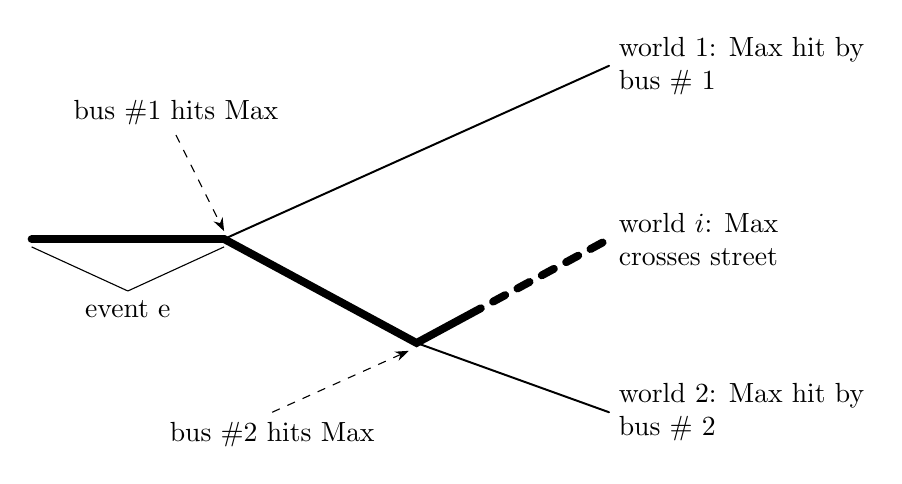
\begin{tikzpicture}
      \tikzmath{
        % x positions
        \x1 = 11;
        \xb1 = 2/9*\x1; \xb2 = 4/9*\x1; \xb3 = 6/9*\x1;
        % y positions
        \y1 = 2/5*\x1; \ymid = 1/2*\y1;
        \yw1 = \y1; \yw2 = 1/2*\y1; \yw3 = 0*\y1; \yb2 = 1/5*\y1;
        % event e
        \xe = 1/2*\xb1; \yediff = \yw2 - \yb2;
        \ye = \yw2 - 1/2*\yediff;
        \enudge = .1;
        \xel = 0; \xer = \xb1; \yen = \yw2 - \enudge;
        % bus 1 description location
        \xbx = 1.5/9*\x1; \xby = 4/5*\y1;
        % bus 2 description location
        \xb9 = 2.5/9*\x1;
      }
      % Paths
      \draw[line width=0.25mm, line cap=round] (\xb1,\ymid) -- (\xb3,\yw1); % world 1
      \draw[line width=1mm, line cap=round, dash pattern=on 175pt off 5pt on 5pt off 5pt on 5pt off 5pt on 5pt off 5pt on 5pt off 5pt on 5pt off 5pt on 5pt off 5pt on 5pt off 5pt on 5pt off 5pt on 5pt off 5pt on 5pt off 5pt on 5pt off 5pt on 5pt off 5pt on 5pt off 5pt on 5pt off 5pt on 5pt off 5pt on 5pt off 5pt on 5pt off 5pt on 5pt off 5pt on 5pt off 5pt] (0,\ymid) -- (\xb1,\ymid) -- (\xb2,\yb2) -- (\xb3,\yw2); % world 2
      \draw[line width=0.25mm, line cap=round] (\xb2,\yb2) -- (\xb3,\yw3); % world 3
      % World descriptions
      \filldraw[black] (\xb3,\yw1) circle (0pt) node[anchor=west, align=left]{world 1: Max hit by \\ bus \# 1};
      \filldraw[black] (\xb3,\yw2) circle (0pt) node[anchor=west, align=left]{world \(i\): Max \\ crosses street};
      \filldraw[black] (\xb3,\yw3) circle (0pt) node[anchor=west, align=left]{world 2: Max hit by \\ bus \# 2};
      % Event
      \draw[] (\xe,\ye) -- (\xel,\yen); % event l
      \draw[] (\xe,\ye) -- (\xer,\yen); % event r
      % Event description
      \filldraw[black] (\xe,\ye) circle (0pt) node[anchor=north, align=left]{event e};
      % Splits
      \filldraw[black, dashed] (\xbx,\xby) circle (0pt) node[anchor=south, align=left]{bus \#1 hits Max};
      \filldraw[black, dashed] (\xb9,\yw3) circle (0pt) node[anchor=north, align=left]{bus \#2 hits Max};
      % Split descriptions
      \draw[-Stealth, dashed] (\xbx,\xby) -- (\xb1,\ymid + \enudge); % bus 2 arrow
      \draw[-Stealth, dashed] (\xb9,\yw3) -- (\xb2 - \enudge,\yb2 - \enudge); % bus 2 arrow
    \end{tikzpicture}
    \caption{
      Continuation path of `Max was crossing the street'. \\
    }
    \label{fig:max-bus}
  \end{figure}

  The thick black line captures \(e\) as \(e\) is allowed to develop, and the changes in angle reflect shifts to alternative possible worlds.

  The dashed line indicates that Max may need to avoids being hit by additional busses in order for \(e\) to develop into an event in which Max crosses the road.

  Still, does \(e\) develop into an event in which Max crosses the road?
  If Max is hit by a bus in \(w\), then surely Max is hit by a bus in all the possible worlds close to \(w\).

  Here we turn to the key property of \citeauthor{Landman:1992wh}'s account which we have so far made without explicit comment:
  Prior to bus \#2 hitting Max in \(v\), we shift to \(u\) where \(u\) is a world which is close to \(v\) rather than \(w\).
  Hence, as the development of \(e\) develops, closeness is understood relative to the development of \(e\), rather than \(e\) itself as \(e\) happened in \(w\).
  So, as Max progresses a little further each time a possible world in which Max crosses the street gets a little closer until, eventually, Max crosses the street.

  This is the core idea of \citeauthor{Landman:1992wh}'s account.
  To borrow a piece of terminology from \textcite{Dowty:1979vq}, \(e\) has sufficient \emph{inertia} to develop in some possible world \(v\), and as \(e\) develops in \(v\), inertia continues to build until Max crosses the road.

  However, an important restriction is placed on shifts to possible worlds.
  Intuitively, Max does not avoid being hit by bus \#\(j\) because Max has the strength to stop as moving bus.
  Yet, a possible world in which Max has the strength to stop a moving bus may be close to the world in which Max is not hit by bus \#\(j - 1\).
  In \citeauthor{Landman:1992wh}'s terminology, the relevant possible worlds in which \(e\) develops must be `reasonable'.
\end{note}

\subparagraph{\pevent{3}}
\label{cha:sec:fcs-def:potential-events}

\begin{note}
  With functional understanding of the progressive in hand, along with \assuPP{}, define \pevent{} to refer to event.
\end{note}

\begin{note}[\pevent{2} definition]
  We define a \pevent{} as follows:
  \begin{restatable}[\pevent{3}]{definition}{definitionPEvent}
    \label{def:potenital-event}
        \cenLine{
      \begin{itemize*}[noitemsep, label=\(\circ\)]
      \item
        Agent: \vAgent{}
      \item
        Action description: \(\alpha\)
      \item
        \mbox{ }
      \end{itemize*}
    }

    \begin{itemize}
    \item
      There is a \pevent{} \(p\) in which \vAgent{} \(\alpha\)s
    \end{itemize}

    \emph{If and only if}:

    \begin{enumerate}[label=]
    \item
      There is some action \(a\) such that both~\ref{def:PE:action} and~\ref{def:PE:prog} are true:
      \begin{enumerate}[label=\alph*., ref=(\alph*)]
      \item
        \label{def:PE:action}
        \vAgent{} may immediately perform \(a\).
      \item
        \label{def:PE:prog}
        \(\text{Prog}(e, \alpha)\) would be true in the event \(e\) of \vAgent{} doing \(a\).
      \end{enumerate}
    \end{enumerate}

    Where \(\text{Prog}(e, \alpha)\) stands for the progressive from of \(\alpha\) when evaluated with respect to \(e\) and \assuPP{} holds for the progressive.%
    \footnote{
      I.e.\ \(\text{Prog}(e, \alpha)\) is true \emph{iff} event \(e\) is an event of \(\alpha\)ing.
      See,~\textcite{Richards:1981wo},~\textcite{Portner:2011vi}, etc.
    }
  \end{restatable}

  In short,~\autoref{def:potenital-event} states that there is a \pevent{} in which an agent performs some action \(\alpha\) just in case there is some action the agent may (immediately) perform which would result in the agent \(\alpha\)ing.
\end{note}

\paragraph{Concluding}

\begin{note}
  Our understanding of `concluding' is that an event in which an agent is concluding some proposition-value pair \(\pv{\phi}{v}\) from some \poP{} \(\Phi\) is just an event such that the event in which the agent concludes \(\pv{\phi}{v}\) from \(\Phi\) is in progress.

  In other worlds, an event of concluding involves some reasoning from some sub-set of the \poP{} \(\Phi\).

  In this respect, an event of concluding need not involve the agent pairing \(\phi\) with \(v\), it need only be the case that if the relevant event went on uninterrupted, then event would develop into an event in which the agent concludes \(\pv{\phi}{v}\) from \(\Phi\), and hence pairs \(\phi\) with \(v\).

  As noted on \autopageref{reasoning-vs-concluding-progressive}, an important distinction between reasoning and concluding is that we don't get this.
  {
    \color{red} Up to here.
  }
\end{note}

\begin{note}
  \begin{observation}[Conclusions without concluding I]
    \label{obs:cds-arb}
    \cenLine{
      \begin{itemize*}[noitemsep, label=\(\circ\)]
      \item
        Agent: \vAgent{}
      \item
        Proposition: \(\phi\)
      \item
        Value: \(v\)
      \item
        \poP{2}: \(\Phi\)
      \item
        Event: \(e\)
      \item
        \mbox{ }
      \end{itemize*}
    }

    \begin{itemize}
    \item
      The following conditional is not necessarily true:
      \begin{itemize}
      \item[\emph{If}:]
        \(e\) is an event in which \vAgent{} concludes \(\pv{\phi}{v}\) from \(\Phi\).
      \item[\emph{Then}:]
        There is some sub-event \(e'\) of \(e\) such that \(e'\) is an event in which \vAgent{} is concluding \(\pv{\phi}{v}\) from \(\Phi\).
      \end{itemize}
    \end{itemize}
  \end{observation}

  \begin{argument}{obs:cds-arb}
    Arbitrary.
  \end{argument}
\end{note}


\begin{note}
  \begin{observation}[Conclusions without concluding II]
    \label{obs:cds-not-cldg}
    \cenLine{
      \begin{itemize*}[noitemsep, label=\(\circ\)]
      \item
        Agent: \vAgent{}
      \item
        Proposition: \(\phi\)
      \item
        Value: \(v\)
      \item
        \poP{2}: \(\Phi\)
      \item
        Event: \(e\)
      \item
        \mbox{ }
      \end{itemize*}
    }

    \begin{itemize}
    \item
      The following conditional is not necessarily true:
      \begin{itemize}
      \item[\emph{If}:]
        \(e\) is an event in which \vAgent{} concludes \(\pv{\phi}{v}\) from \(\Phi\).
      \item[\emph{Then}:]
        There is some sub-event \(e'\) of \(e\) such that \(e'\) is an event in which \vAgent{} is concluding \(\pv{\phi}{v}\) from \(\Phi\).
      \end{itemize}
    \end{itemize}
  \end{observation}

  \begin{argument}{obs:cds-not-cldg}
    It need not be the case that \citeauthor{Maksimova:1977un} knew there are exactly five intermediate logics that have the interpolation property was a \fc{} before proving such (\cite[cf.][]{Maksimova:1977un}).

    However, the same hold for when the agent pairs \(\phi\) with \(v\).
    For, the agent need not know they would repeat the reasoning.
    To \illu{0}, consider being guided through a complex argument.
    Follow along, and conclude.
    At each step, do the reasoning, the guide highlights which sub-conclusions to draw.
    However, guide goes away.
    And, given complexity, no repetition without guide.
  \end{argument}
\end{note}

\section{Reasoning}
\label{sec:reasoning-1}

\begin{note}
  \color{blue}
  Conclusion is an instance of reasoning.
  No strict constraints on reasoning.
  However, \tR{}.
\end{note}

\begin{note}
  We have assumed that concluding is an instance of reasoning, and more specifically that concluding involves an agent reasoning from some \poP{} to some conclusion, where both premises and conclusions are understood in terms of proposition-value pairings.
  In this respect, the assumptions we have made place constraints on certain instances of reasoning.
  However, aside from understanding reasoning in terms of proposition-value pairings, we do not place further constraints on reasoning.

  Note, the absence of placed constraints does not imply that reasoning is unconstrained.
  Rather, we adopt a neutral stance on what may count as instance of reasoning.
\end{note}

\begin{note}[No constraints]
  To illustrate, consider the contrast between \citeauthor{Broome:2013aa}'s (\citeyear{Broome:2013aa}) rule following account of reasoning and \citeauthor{Wedgwood:2006ui}'s (\citeyear{Wedgwood:2006ui}) reason-based account of reasoning.

  \citeauthor{Broome:2013aa}'s rule following account of reasoning is unconstrained in terms of the rules an agent may follow.
  This aspect  of \citeauthor{Broome:2013aa}'s account is highlighted in the following passage:

  \begin{quote}
    [S]hould we exclude this bizarre rule: from the proposition that it is raining and the proposition that if it is raining the snow will melt, to derive the proposition that you hear trumpets.
    Following this rule would lead you to believe you hear trumpets when you believe it is raining and believe that if it is raining the snow will melt.
    If you did this, should we count you as reasoning?

    I think we should.
    If you derive this conclusion by operating on the premises, following the rule, we should count you as reasoning.
    \dots
    I think we should not impose a limit on rules.%
    \mbox{}\hfill\mbox{(\citeyear[233]{Broome:2013aa})}
  \end{quote}

  By constraint, \citeauthor{Wedgwood:2006ui}'s reason-based account of reasoning:

  \begin{quote}
    Reasoning, I shall assume, is the process of \emph{revising ones beliefs or intentions, for a reason}.%
    \mbox{ }\hfill\mbox{(\citeyear[600]{Wedgwood:2006ui})}
  \end{quote}

  \citeauthor{Wedgwood:2006ui} understands reasons in terms of intelligibility.%
  \footnote{
    Strictly, \citeauthor{Wedgwood:2006ui} understanding reasoning in terms of dispositions that respond to what `rationalizes' (\citeyear[672]{Wedgwood:2006ui}) and \citeauthor{Wedgwood:2006ui} considers `rationalizes' and  `makes intelligible' as equivalent.
    Therefore, the following conditional, states a sufficient rather than necessary condition which leads to \citeauthor{Wedgwood:2006ui}'s assumption, rather than being an expansion of what \citeauthor{Wedgwood:2006ui}'s assumption amounts to.
    I find this particularly confusion.
  }

  \begin{quote}
    If a set of antecedent mental states makes it rational for one to form a new belief or intention, then those antecedent mental states are surely of a suitable type and content so that it is \emph{intelligible} that they could represent one's reason for forming that belief or intention.\newline
    \mbox{ }\hfill\mbox{(\citeyear[662]{Wedgwood:2006ui})}
  \end{quote}

  Now, perhaps the presence of the rule in \citeauthor{Broome:2013aa}'s example makes it intelligible that the agent concludes that they hear trumpets from the relevant premises.
  However, there is also a clear sense in which the reasoning in \citeauthor{Broome:2013aa}'s example in \emph{unintelligible}.

  \citeauthor{Wedgwood:2006ui} provides the following contrasts to clarify their understanding of intelligibility:

  \begin{quote}
    [T]he belief that the \emph{Oxford Dictionary of National Biography} says that Hume died in 1776 seems a mental state of a suitable type and content so that it could intelligibly represent one's reason for believing that Hume died in 1776.
    On the other hand, it is not (except in the presence of some rather extraordinary background beliefs) a mental state of a suitable type and content so that it could intelligibly represent one's reason for believing that every even number is the sum of two primes.%
    \mbox{ }\hfill\mbox{(\citeyear[662]{Wedgwood:2006ui})}
  \end{quote}

  Does the rules that the agent follows in \citeauthor{Broome:2013aa}'s example count as a sufficiently extraordinary background belief?
  Indeed, \citeauthor{Broome:2013aa} do not require that, in general, an agent has beliefs concerning of the rules they follow in reasoning (\citeyear[Cf.][\S13.2]{Broome:2013aa}).
\end{note}

\begin{note}
  By refraining from placing any further constraints on reasoning we remain neutral on whether an unconstrained approach to reasoning is line with \citeauthor{Broome:2013aa} is correct, or whether a constrained approach to reasoning in line with \citeauthor{Wedgwood:2006ui} is correct.

  Still, in general, we aim to consider instances of reasoning (and concluding) which are intuitive.
  Hence, we hope that the instances of reasoning we consider are compatible with whatever way reasoning is understood.
\end{note}

\section{Attitudes}

\begin{note}
  Conclusion of reasoning is a proposition-value pairing.
  In general, this does not provide information about the attitude that the agent holds toward the proposition.

  For example, conclude that \(\phi\) has value `true'.
  Conclusion may amount to knowledge, belief, or some other veridical attitude.

  We will have little interest in propositional attitudes.
  Our interest is in concluding, and it is rarely the case that one concludes that they have some attitude toward a proposition.
  Conclude that the cat is on the mat, do not conclude that I believe the cat is on the mat.

  Set aside interest in attitudes when concluding.
  Interest will be in proposition-value-premises pairings for agent.
\end{note}

\begin{note}
  Some difficulty in understanding answers to \qWhy{} and agent concludes.
  Evaluations are not attitudes.
  However, attitude entail evaluations.
\end{note}

\begin{note}
  \citeauthor{Davidson:1963aa}, reasons in terms of attitudes.

  \begin{quote}
    \emph{R} is a primary reason why an agent performed the action \emph{A} under the description \emph{d} only if \emph{R} consists of a pro attitude of the agent toward actions with a certain property, and a belief of the agent that \emph{A}, under the description \emph{d}, has that property.%
    \mbox{ }\hfill\mbox{(\citeyear[687]{Davidson:1963aa})}
  \end{quote}

  However, foundation of (pro-)attitude is proposition-value pairing.
  So, pro-attitude, evaluation with something like desire, and belief with evaluation of true.

  In this respect, \citeauthor{Davidson:1963aa} is agent neutral.
  Primary reason is not seen from agent's point of view.
  Instead, from our point of view.
  However, entailed (or corresponding) account from agent's point of view.%
  \footnote{
    Clearer given principle \citeauthor{Smith:1987vk} derives from the Humean Theory of Motivation, as captured by~\ref{Smithh:HtM:2}:
    \begin{quote}
      \begin{enumerate}[label=\textsc{P1}., ref=(\textsc{P1})]
      \item
        \label{Smithh:HtM:2}
        Agent A at t has a motivating reason to \(\phi\) only if there is some \(\psi\) such that, at t, A desires to \(\psi\) and believes that were he to \(\phi\) he would \(\psi\).%
        \mbox{ }\hfill\mbox{(\citeyear[36]{Smith:1987vk})}
      \end{enumerate}
    \end{quote}

    Understand desire of A to \(\psi\) in terms of the evaluation of \(\psi\) as desirable, and the belief as evaluating if do \(\phi\) then \(\psi\).

    \citeauthor{Smith:1987vk} suggests comparison to \textcite{Davidson:1963aa}.
    Note, in particular \citeauthor{Smith:1987vk}'s use of `motivating reason' is equivalent to \citeauthor{Davidson:1963aa}'s use of `primary reason' rather than `reason'.
  }

  So, \citeauthor{Davidson:1963aa}'s constraint in terms of cause is a little more delicate.
\end{note}

\begin{note}
  Hope this is straightforward.%
  \footnote{
    Discussion by \citeauthor{Collins:1997wn} and \citeauthor{Dancy:2000aa}.
  }
  Contrast is possible, from agent's point of view it is that agent has relevant propositional attitudes.

  Consider the follow passage from \citeauthor{Hume:2011aa}'s \hyperlink{cite.Hume:2011aa}{Treatise}:

  \begin{quote}
    'Tis also obvious, that this emotion rests not here, but making us cast our view on every side, comprehends whatever objects are connected with its original one by the relation of cause and effect.
    Here then reasoning takes place to discover this relation; and according as our reasoning varies, our actions receive a subsequent variation.
    But 'tis evident in this case, that the impulse arises not from reason, but is only directed by it.
    'Tis from the prospect of pain or pleasure that the aversion or propensity arises towards any object: And these emotions extend themselves to the causes and effects of that object, as they are pointed out to us by reason and experience.%
    \mbox{ }\hfill\mbox{(\hyperlink{cite.Hume:2011aa}{T.2.3.3})}
  \end{quote}

  The passage captures means-end \emph{reasoning}.
  Evaluate an object according to the prospect of pain or pleasure.
\end{note}

%%% Local Variables:
%%% mode: latex
%%% TeX-master: "master"
%%% End:


\chapter{\ros{3}}
\label{cha:ros}


\begin{note}
  \ros{3} capture the way in which a \prop{0}-\val{0} pair \(\pv{\phi}{v}\) `follows from' some \pool{} \(\Phi\), from an \agpe{}.
  Where the `following from' relation contrasts with `from' in the sense that  an agent concludes \(\pv{\phi}{v}\) `from' \(\Phi\).
\end{note}


\begin{note}
  Broad idea.

  In turn, \ros{3} are answers to \qWhy{}, and if \issueConstraint{} holds, for any \ros{} which answers \qWhy{} there is some event where agent concludes.
\end{note}


\begin{note}
  Specifying \ros{} in any significant detail is beyond the scope of this document.
  \issueInclusion{} is understood as a (plausible) constraint on theories about the why and how of reasoning rather than the details of any given theory.
  Instead, we characterise \ros{} by two ideas, and anything which satisfies these two ideas in the details of a given theory may be understood as a \ros{}.
\end{note}


\section{\supportI{}}
\label{cha:ros:I}


\begin{note}
  The role of \supportI{} is to characterise when a \ros{} holds between some \prop{0}-\val{0} pair and \pool{} \emph{given} an event in which the agent concludes the \prop{0}-\val{0} pair from the \pool{}.

  \begin{idea}[\supportI{}]
    \label{idea:support}
    \vspace{-\baselineskip}
    \begin{itenum}
    \item[\emph{If}:]
      \(\ed{}\) is an event in which \vAgent{} concludes \(\pv{\phi}{v}\) from \(\Phi\).
    \item[\emph{Then}:]
      When \vAgent{} \eval{1} \(\phi\) as having value \(v\): %as a \se{0} of \(\ed{}\):
      \begin{itemize}
      \item
        A \emph{\ros{}} between \(\pv{\phi}{v}\) and \(\Phi\) holds, from \agpe{\vAgent{}'}.
      \end{itemize}
    \end{itenum}
    \vspace{-\baselineskip}
  \end{idea}

  \noindent%
  In short, \supportI{} states that a \ros{} between \(\pv{\phi}{v}\) and \(\Phi\) holds form an \agpe{} when the agent concludes \(\pv{\phi}{v}\) from \(\Phi\).%
  \footnote{
    The existence of a \ros{} is restricted to the sub-event when the agent \evals{} \(\phi\) as having \val{} \(v\) as a concludes event may span the \agents{} reasoning to \(\pv{\phi}{v}\) from \(\Phi\) (\autoref{assu:ConRea}).
  }

  The motivation for \supportI{} is straightforward:
  The role of \ros{0} a \ros{} between \(\pv{\phi}{v}\) and \(\Phi\) is to abstractly capture the way in which \(\pv{\phi}{v}\) `follows from' \(\Phi\) from the \agpe{}.
  And, if an agent concludes \(\pv{\phi}{v}\) from \(\Phi\), then \(\pv{\phi}{v}\) `follows from' \(\Phi\) from the \agpe{}.

  In other words, the \ros{} between \(\pv{\phi}{v}\) and \(\Phi\) just captures whatever it is, for the agent, that led to the agent concluding \(\pv{\phi}{v}\) from \(\Phi\).
\end{note}


\begin{note}
  \supportI{} ensures a \ros{} between \pv{\propM{\rootsCon{}}}{\valI{True}} and some \pool{} which captures the \agents{} understanding of factorisation or the quadratic formula holds when the agent makes the relevant conclusion in \scen{1}~\ref{illu:gist:roots:F}~and~\ref{illu:gist:roots:QF}.
  Likewise, \supportI{} ensures a \ros{} between \pv{\propI{What Pritcher said was a sign}}{\valI{True}} and some \pool{} \(\Psi\) holds from \agpe{Fox's} in \autoref{scen:countS} when Fox responds to `I come from Miran' with `Miran is early this year'.
\end{note}


\begin{note}
  Our characterisation of \ros{} by \supportI{} rests on the way in which we understand conclusions.
  In particular, \supportI{} allows for \ros{} to hold between any \prop{0}-\val{0}-\pool{0} pair, so long as the agent concludes the relevant \prop{0} has the specified \val{0} from the given \pool{}, or the \prop{0}-\val{0} pair is a \fc{} from the \pool{}.
  Hence, a \ros{} may hold between, e.g., \pv{\propI{Fish are mammals}}{\valI{True}} and some \pool{} from the \agpe{}.

  If the way in which conclusions are understood is restricted, the \ros{} as characterised are likewise restricted.
  And, that \ros{1} hold between certain \prop{0}-\val{0} pairs and \pool{1} is important for the argument to follow, not that \ros{1} may hold between arbitrary \prop{0}-\val{0} pairs and \pool{1}.
  The benefit of the characterisation given is simplicity.
  For example, I expect the argument to follow is compatible with restricting \ros{} to justified conclusions.%
  \footnote{
    Or, for example, properly based.
    For relevant concerns see (\cite{Schaffer:2010vq}) --- and also (\cite{Bondy:2018tk}) for counterpoint.
  }
\end{note}



\section{\wit{3} for \ros{1}}
\label{cha:ros:W}


\begin{note}
  With \supportI{}, and hence some characterisation of \ros{}, in hand we define a `\wit{0}' for \ros{} between \(\pv{\phi}{v}\) and \(\Phi\).
  In full:

  \begin{definition}[A \wit{0} for a \ros{1}]%
    \label{def:witnessing}%
    \vspace{-\baselineskip}
    \begin{itemize}
    \item
      An event \(\ed{\ast}\) is \emph{\wit{0}} for a \ros{} between \(\pv{\phi}{v}\) and \(\Phi\), for \vAgent{} throughout an event \(\ed{}\).
    \end{itemize}

    \emph{If and only if:}

    \begin{itemize}
    \item
      \(\ed{\ast}\) is an event in which \vAgent{} concludes \(\pv{\phi}{v}\) from \(\Phi\).
    \item
      \(\ed{\ast}\) occurs prior to or at the same time as \(\ed{}\).
    \end{itemize}
    \vspace{-\baselineskip}
  \end{definition}

  \noindent%
  In short, a \wit{} for a \ros{} between \(\pv{\phi}{v}\) and \(\Phi\) is some (extant) event in which the agent concludes \(\pv{\phi}{v}\) from \(\Phi\).

  And, if an agent has concluded \(\pv{\phi}{v}\) from \(\Phi\), we say the agent `has a \wit{}' for a \ros{} between \(\pv{\phi}{v}\) and \(\Phi\).
\end{note}


\begin{note}
  An important, but trivial, case of \autoref{def:witnessing} is when an agent concludes \(\pv{\phi}{v}\) from \(\Phi\).
  For, if an agent concludes \(\pv{\phi}{v}\) from \(\Phi\) then it is immediate that there is some event in which the agent concludes \(\pv{\phi}{v}\) from \(\Phi\) --- the very same event --- and hence the agent has a \wit{} for the \ros{} between \(\pv{\phi}{v}\) and \(\Phi\).
\end{note}



\section{\supportII{}}
\label{cha:ros:II}


\begin{note}
  The role of \supportII{} is to characterise a sufficient condition for a \ros{} to hold between some \prop{0}-\val{0} pair and \pool{} from an \agpe{} \emph{regardless of} an event in which the agent concludes the \prop{0}-\val{0} pair from the \pool{}.

  In \autoref{cha:intro} we broadly motivated the idea of such \ros{}.
  In detail, we use the idea of a \fc{0} to narrowly ensure certain \ros{1} exist:

  \begin{idea}[\supportII{}]%
    \label{idea:support:possible}%
    \vspace{-\baselineskip}
    \begin{itenum}
    \item[\emph{If}:]
      \(\pv{\phi}{v}\) is a \fc{0} from \(\Phi\) for \vAgent{} throughout \(\ed{}\).
    \item[\emph{Then}:]
      A \ros{} between \(\pv{\phi}{v}\) and \(\Phi\) holds from \agpe{\vAgent{}'} throughout \(\ed{}\).
    \end{itenum}
    \vspace{-\baselineskip}
  \end{idea}

  \noindent%
  A \ros{} is designed to abstractly capture the way in which some \prop{0}-\val{0} pair `follows from' some \pool{} from an \agpe{}.
  \supportII{}, states that \(\pv{\phi}{v}\) being a \fc{} from \(\Phi\) is sufficient for a \ros{} between \(\pv{\phi}{v}\) and \(\Phi\) to hold from the \agpe{}.
\end{note}


\begin{note}
  \noindent%
  Expanded with the definition of a \fc{}, \supportII{} reads:
  \begin{itenum}
  \item[\emph{If}:]
    \begin{itemize}
    \item
      Throughout \(\ed{}\) there is some action \(a\) \vAgent{} may immediately perform such that both \ref{def:fc:act} and \ref{def:fc:result} are true:
      \begin{enumerate}[label=\alph*., ref=(\alph*)]
      \item
        For each \prop{0}-\val{0} pair \(\pv{\phi'}{v'}\) in \(\Phi\), \vAgent{} \evals{} \(\phi'\) as having value \(v'\) prior to doing \(a\).
      \item
        The event \(e^{\sharp}_{d^{\sharp}}\) in which \vAgent{} does \(a\) is an event in which \vAgent{} is concluding \(\pv{\phi}{v}\) from \(\Phi\).
      \end{enumerate}
    \end{itemize}
  \item[\emph{Then}:]
    A \ros{} between \(\pv{\phi}{v}\) and \(\Phi\) holds from \agpe{\vAgent{}'} throughout \(\ed{}\).
  \end{itenum}

  \noindent%
  In short, something about the \agpe{\agents{} present} already secures anything that is required to hold from the \agpe{} when the agent concludes \(\pv{\phi}{v}\) from \(\Phi\).
\end{note}


\begin{note}
  \supportII{} captures the idea that a \ros{} between \pv{\propM{\rootsCon{}}}{\valI{True}} and some \pool{} which captures their understanding of factorisation or the quadratic formula holds when the agent is concluding \pv{\propM{\rootsCon{}}}{\valI{True}} from the relevant \pool{} in \scen{1}~\ref{illu:gist:roots:F}~and~\ref{illu:gist:roots:QF}.

  Likewise, \supportII{} states a \ros{} holds between the relevant \prop{0}-\val{0} pair and \pool{} for each of the \fc{1} in \autoref{cha:fcs}.%
  \footnote{
    Perhaps one may say a good puzzle of the kind given in \autoref{scen:fc:chick} is a puzzle in which a \ros{} already holds between the intended solution and some \pool{} for the agent (after reading the puzzle) and obtaining a \wit{} for the \ros{} is enjoyable.
  }

  In \autoref{scen:countS}, by contrast, \supportII{} does state a \ros{} between \pv{\propI{What Pritcher said was a sign}}{\valI{True}} and some \pool{} \(\Psi\) holds \emph{prior to} Fox's conclusion of \pv{\propI{What Pritcher said was a sign}}{\valI{True}} from \(\Psi\).
  For, for example, Pritcher may have said `I come from Wilau' and failed to sign and hence \pv{\propI{What Pritcher said was a sign}}{\valI{True}} was not a \fc{} from \(\Psi\).

  And, \supportII{} does not states a \ros{} holds between the relevant \prop{0}-\val{0} pair and \pool{} for any absent \fc{1} in \autoref{cha:fcs}.
\end{note}


\begin{note}
  Additional example.

  \begin{scenario}[Fibonacci numbers]%
    \label{scen:fc:fib}%
    The Fibonacci numbers are recursively defined as follows:

    \[
      F_{n} = \left\{
        \begin{array}{ll}
          0 & \text{if } n = 0 \\
          1 & \text{if } n = 1 \\
          F_{n-1} + F_{n-2} & \text{if } n > 1 \\
        \end{array}
      \right.
    \]
  \end{scenario}

  \begin{enumerate}[label=C\thescenarioCounter., ref=(C\thescenarioCounter)]
  \item
    \label{scen:fc:fib:c}
    \pv{\propI{The sixth number in the Fibonacci sequence is 5}}{\valI{True}}
  \end{enumerate}
  %
  Given an understanding of \(f\) and sufficient motivation, an agent may do some action and be concluding \pv{\propI{The six number in the Fibonacci sequence is 5}}{\valI{True}}.
  Hence, \pv{\propI{The six number in the Fibonacci sequence is 5}}{\valI{True}} is a \fc{} from some \pool{}.
  Hence, so long as the action is available a \ros{} holds between \pv{\propI{The six number in the Fibonacci sequence is 5}}{\valI{True}} and some \pool{} which captures the \agents{} understanding of \(f\).

  Though, \pv{\propI{The sixtieth number in the Fibonacci sequence is 1548008755920}}{\valI{True}} need not be \fc{0}.
  For, even if one uses memos, the \emph{sixtieth} number requires a lot of work, and the agent may not have sufficient resources to make the conclusion.
  So, it need not be the case that a \ros{} holds by \supportII{}.
\end{note}



\section[Some notes]{Some notes \hfill (Optional)}


\begin{note}
  This section contains three optional notes.

  The first note contrasts our understanding of the connexion between \ros{1} and an event in which an agent concludes to \citeauthor{Boghossian:2014aa}'s understanding of the connexion between `support' an event in which an agent infers.

  The second note draws a parallel between our \supportII{} and \citeauthor{Goldman:1979ui}'s account of \emph{ex ante} justification.

  The third note considers the possibility of \ros{} occurring within \ros{} and states we ignore the possibility.
\end{note}



\subsection{\supportI{} and \citeauthor{Boghossian:2014aa} Taking Condition}


\begin{note}
  \supportI{} is similar to, but distinct from,~\citeauthor{Boghossian:2014aa}'s Taking Condition:%
  \footnote{
    Strictly,~\citeauthor{Boghossian:2014aa} states the Taking Condition in terms of inferring.
    I.e., the Taking Condition reads: `Inferring necessarily involves the thinker \emph{taking} \dots'
    However, as \citeauthor{Boghossian:2008vf} is interested in conclusions, an event in which an agent infers (in~\citeauthor{Boghossian:2014aa} sense) is an event in which an agent concludes (in our sense).
  }

  \begin{quote}
    (Taking Condition):
    [An event in which an agent concludes] necessarily involves the thinker \emph{taking} his premises to support his conclusion and drawing his conclusion because of that fact.%
    \mbox{}\hfill\mbox{(\citeyear[5]{Boghossian:2014aa})}
  \end{quote}

  \noindent%
  For, `taking' is understood by \citeauthor{Boghossian:2014aa} to be component of the agent's reasoning.
  \citeauthor{Boghossian:2014aa} illustrates the Taking Condition as follows:
  %
  \begin{quote}
    On waking up one morning I recall that:

    \begin{enumerate}[label=(\arabic*), ref=(\arabic*), series=BogEx]
    \item
      \label{BogEx:1}
      It rained last night.
    \end{enumerate}

    I combine this with my knowledge that

    \begin{enumerate}[label=(\arabic*), ref=(\arabic*), resume*=BogEx]
    \item
      \label{BogEx:2}
      If it rained last night, then the streets are wet.
    \end{enumerate}

    to conclude:

    So,

    \begin{enumerate}[label=(\arabic*), ref=(\arabic*), resume*=BogEx]
    \item
      \label{BogEx:3}
      The streets are wet.
    \end{enumerate}
    This belief then affects my choice of footwear.%

    [\dots M]y inferring from~\ref{BogEx:1} and~\ref{BogEx:2} to~\ref{BogEx:3} must involve my arriving at the judgment that~\ref{BogEx:3} in part \emph{because} I \emph{take} the presumed truth of~\ref{BogEx:1} and~\ref{BogEx:2} to provide support for~\ref{BogEx:3}.%
    \mbox{ }\hfill\mbox{(\citeyear[2,4]{Boghossian:2014aa})}
  \end{quote}
  %
  Hence, for \citeauthor{Boghossian:2014aa}, the Taking Condition captures something \emph{in addition} to~\ref{BogEx:3} being a conclusion from a \pool{} which includes~\ref{BogEx:1} and~\ref{BogEx:2}.

  In contrast, we do not require that a \ros{} has any particular role \emph{for the agent} in event in which an agent concludes \(\pv{\phi}{v}\) from \(\Phi\).
  If an agent concludes~\ref{BogEx:3} from~\ref{BogEx:1} and~\ref{BogEx:2}, then a \ros{} holds between~\ref{BogEx:3} and \(\{\ref{BogEx:1}, \ref{BogEx:2}\}\).
  However, the \ros{} between~\ref{BogEx:3} and \(\{\ref{BogEx:1}, \ref{BogEx:2}\}\) need not itself have a role in the \agents{} conclusion of~\ref{BogEx:3} from \(\{\ref{BogEx:1}, \ref{BogEx:2}\}\).%
  \footnote{
    Also, about the type of reasoning by which the agent concludes.
    This comes from \textcite{Boghossian:2008vf,Boghossian:2012vb}.
    Rule following, taking gets account of rule.
  }

  \label{wrightSimp}%
  To illustrate, consider \citeauthor{Wright:2014tt}'s (\citeyear{Wright:2014tt}) `Simple Proposal':
  %
  \begin{quote}
    % [C]onsider instead the proposal, not that the status of the transition as inferential depends on the thinker's judgments about his reasons, but that it depends on \emph{what his reasons are}.
    % We want his acceptance of the premises to supply his \emph{actual} reasons for accepting the conclusion.
    % [\dots]
    %
    % Call this the Simple Proposal.
    % It says that a thinker infers q from p\(_{1}\) \(\cdots\) p\(_{\text{n}}\) when he accepts each of p\(_{1}\) \(\cdots\) p\(_{\text{n}}\), moves to accept q, and does so for the reason that he accepts p\(_{1}\) \(\cdots\) p\(_{\text{n}}\).%
    [The Simple Proposal] says that a thinker infers q from p\(_{1}\) \(\cdots\) p\(_{\text{n}}\) when he accepts each of p\(_{1}\) \(\cdots\) p\(_{\text{n}}\), moves to accept q, and does so for the reason that he accepts p\(_{1}\) \(\cdots\) p\(_{\text{n}}\).%
    \mbox{}\hfill\mbox{(\citeyear[33]{Wright:2014tt})}
  \end{quote}
  %
  \citeauthor{Wright:2014tt}'s proposal is that the relation between a conclusion and some \pool{} need not be part of what moves the agent to conclude the conclusion from the \pool{}.
  Hence, \citeauthor{Wright:2014tt} denies that reasoning must involve a state which connects premises to conclusions.
  So, \citeauthor{Wright:2014tt} denies \citeauthor{Boghossian:2008vf}'s Taking Condition on inference  (\citeyear[Cf.][33-34]{Wright:2014tt}).

  \supportI{} is compatible with \citeauthor{Wright:2014tt}'s Simple Proposal as \supportI{} only entails a \ros{} holds between \(\pv{\propM{q}}{\valI{True}}\) and a \pool{} containing \(\pv{\propM{p_{1}}}{\valI{True}}\), \(\cdots\) \(\pv{\propM{p_{n}}}{\valI{True}}\).%
  \footnote{
    Still, there is an important between~\supportI{} and \citeauthor{Wright:2014tt}'s Simple Proposal.
    For,~\supportI{} is an entailment, while \citeauthor{Wright:2014tt}'s Simple Proposal is an identity statement.
    Inferring, on the Simple Proposal, is an agent accepting some conclusion for the reason that they accept premises from some \pool{}.
    \supportI{} does not entail that concluding is nothing more than moving to accept \(\pv{\phi}{v}\) as a result of accepting each element of \(\Phi\).
  }\(^{,}\)%
  \footnote{
    There are various other objections to~\citeauthor{Boghossian:2014aa}'s Taking Condition.

    For example,~\citeauthor{Hlobil:2014tq} argues against the Taking Condition as it distracts from what accounts of reasoning out to explain, rather than arguing against the Taking Condition directly.
    Likewise, \citeauthor{McHugh:2016vp} present and summarise various objections to \emph{interest} with the Taking Condition.

    In particular,~\supportI{} is closer to what \citeauthor{McHugh:2016vp} term the `Consequence Condition': \textquote{Inferring q from p entails taking p to support q}.
    (\citeyear[316]{McHugh:2016vp})
    And, as \citeauthor{McHugh:2016vp} observe, the condition is \textquote{consistent with the idea that in inference we take our premises to support our conclusion just in virtue of reasoning from the former to the latter}.
    (\citeyear[316]{McHugh:2016vp})

    \citeauthor{McHugh:2016vp} suggest the arguments they consider against the Taking Condition `put pressure' on the Consequence Condition (\citeyear[327]{McHugh:2016vp}).
    However, these arguments concern interest, rather than whether condition is true.
    And, we, uh, have interest in \ros{1}\dots
  }
\end{note}

% \begin{note}
%   \color{red}
%   Humpty Dumpty arbitrary chooses for `glory' to mean `a nice knock-down argument' (\cite[190]{Carroll:2009aa}).
% \end{note}


\subsection{\supportII{} and \citeauthor{Goldman:1979ui}'s account of \emph{ex ante} justification}


\begin{note}
  From a structural perspective, our approach to characterising \ros{1} without a given an event in which the agent concludes is similar to \citeauthor{Goldman:1979ui}'s account of \emph{ex ante} justification in terms of \emph{ex post} justification.%
  \footnote{
    \citeauthor{Goldman:1979ui}'s notions of \emph{ex ante} and \emph{ex post} justification is similar to the distinction between doxastic and propositional justification (see \cite{Firth:1978vi} and \cite[esp.\ fn.1]{Silva:2020aa}).

    Given the parallels between \ros{1} and \emph{ex ante} justification, may think of \ros{1} in line with propositional justification.
  }%
  \(^{,}\)%
  \footnote{
    \citeauthor{Turri:2010aa} (\citeyear{Turri:2010aa}) provides similar account.
    However, \citeauthor{Turri:2010aa} does not hold that this is sufficient.
  }

  Here's a paraphrase of \citeauthor{Goldman:1979ui}'s account of \emph{ex post} justification:
  \begin{quote}
    Person \emph{S} is \emph{ex post} justified in believing \emph{p} when \emph{S} believes \emph{p}, and we say \emph{S}' believing \emph{p} is~justified.%
    \mbox{ }\hfill\mbox{(\citeyear[Cf.][21]{Goldman:1979ui})}
  \end{quote}
  % 
  And here's \citeauthor{Goldman:1979ui}'s account of \emph{ex ante} justification:
  % 
  \begin{quote}
    Person \emph{S} is \emph{ex ante} justified in believing \emph{p} at \emph{t} if and only if there is a reliable belief-forming operation available to \emph{S} which is such that if \emph{S} applied that operation to his total cognitive state at \emph{t}, \emph{S} would believe pat \emph{t}-plus-delta (for a suitably small delta) and that belief would be \emph{ex post} justified.%
    \mbox{ }\hfill\mbox{(\citeyear[21]{Goldman:1979ui})}
  \end{quote}
  %
  In a broad stroke, someone is \emph{ex ante} justified in believing \emph{p} at \emph{t} just in case there is some action the person may immediately do and as a result of doing the action, the person is \emph{ex post} justified in \emph{p}.

  Likewise, if \support{} characterises an \emph{ex post} \ros{0} and \supportII{} characterises an \emph{ex ante} \ros{0} we may say, in a broad stroke, an \emph{ex ante} \ros{} holds from an \agpe{} just in case there is some action the person may immediately do and as a result of doing the action a \emph{ex post} \ros{} holds from the \agpe{}.

  There is, however, a small difference:
  \citeauthor{Goldman:1979ui} defines \emph{ex ante} justification in terms of \emph{ex post} justification, whereas we only provide a sufficient condition for an \emph{ex ante} \ros{} in terms of an \emph{ex post} \ros{}.
\end{note}


\subsection{\ros{3} which contain \ros{1}}


\begin{note}
  A \ros{} holding between \(\pv{\phi}{v}\) and \(\Phi\) is a way things are.
  Therefore, it is possible for an agent to \eval{} the \prop{} \propI{A \ros{} between \(\pv{\phi}{v}\) and \(\Phi\)} as \valI{True}, \valI{Possible}, \valI{Desired}, and so on\dots.

  Hence, it is possible for both \ref{Embed:no} and \ref{Embed:yes} to occur:

  \begin{enumerate}[label=\arabic*., ref=(\arabic*)]
  \item
    \label{Embed:no}
    A \ros{0} between \(\pv{\phi}{v}\) and \(\Phi\) holds from \agpe{an \agents{}}.
  \item
    \label{Embed:yes}
    A \ros{0} between \(\pv{\psi}{v'}\) and \(\Psi\) holds from \agpe{an \agents{}}, where \(\Psi\) contains:

    \pv{\propI{A \ros{} between \(\pv{\phi}{v}\) and \(\Phi\) holds from \agpe{my}}}{\valI{True}}
  \end{enumerate}

  Now, in the case of \ref{Embed:yes}, it is not necessarily the case that a A \ros{0} between \(\pv{\phi}{v}\) and \(\Phi\) holds from \agpe{the}.
  For example, if an agent may think the answer to the puzzle of \autoref{illu:fc:chess:II} is a \fc{}, though in reality the agent isn't particularly good at thinking through chess problems.

  When we speak of \ros{} we do not consider \ros{} which are embedded within \ros{}.
  Hence, we do not consider \ros{} which are embedded within \ros{} as answers to \qWhy{}.%
  \footnote{
    Though, \ref{Embed:no} and \ref{Embed:yes} may occur simultaneously, and \ref{Embed:no} may be the case, in part, due to \ref{Embed:yes} being the case.
    However, as this takes some effort to think about, we will not (directly, at least) consider cases where \ref{Embed:no} is the case due to \ref{Embed:yes} being the case.
  }

  Relevant definitions could be refined to explicitly exclude embedded \ros{1}.
  However, in this case I think ignoring is preferable to precision.
\end{note}



\section*{Summary}


\begin{note}
  \ros{}.
  For the remainder of this document only the definition of a \wit{} and \supportII{} are of particular interest.
  \supportI{} ensures our detailed account of \ros{} is in line with the way \ros{} were introduced in \autoref{cha:intro} and to help motivate \supportII{}.
\end{note}


% \begin{note}
%   It need not be the case that an agent has a \wit{0} for a \ros{0} in order for \ros{} to be involved in answering \qWhyV{}.

%   For, suppose an agent does not have a \wit{0} for the \ros{} between \(\pv{\psi}{v'}\) and \(\Psi\).
%   The upshot of the distinction between~\ref{Embed:no} and~\ref{Embed:yes} is as follows:

%   \begin{itemize}
%   \item
%     If the \ros{0} of \ref{Embed:no} is, in part, an answer to \qWhyV{} then the \ros{0} is a counterexample to \issueConstraint{}.
%   \item
%     If the \ros{0} of \ref{Embed:yes} is, in part, an answer to \qWhyV{} then the \ros{0} is \emph{not} a counterexample to \issueConstraint{}.
%   \end{itemize}

%   The difference is \emph{the way in which} the \ros{} functions with respect to the agent pairing \(\phi\) with \(v\).
%   Whether the \ros{} functions as a premise when the agent concludes \(\pv{\phi}{v}\), or whether the \ros{} functions in a way that is different to a premise.
% \end{note}

% \begin{note}
%   \begin{itemize}
%   \item
%     \(\pv{\phi}{v}\) is supported by \(\Phi\), from the \agpe{}.
%   \item
%     \(\pv{\psi}{v'}\) is supported, in part, by [the way in which \(\pv{\phi}{v}\) is supported by \(\Phi\), from the \agpe{}], from the \agpe{}.
%   \item
%     The way in which \(\pv{\psi}{v'}\) is supported, in part, by the \agpe{} on [the way in which \(\pv{\phi}{v}\) is supported by \(\Phi\), from the \agpe{}].
%   \end{itemize}

%   \ros{} of \ref{Embed:no} is a \ros{} which holds from the \agpe{}
%   \ros{} of \ref{Embed:yes} is a \ros{} which holds from the \agpe{}, from the \agpe{}.
%   Expanded a little more carefully, the primary \ros{1} of \ref{Embed:no} and \ref{Embed:yes} are paraphrased as capturing:
%   %   
%   \begin{itemize}
%   \item
%     The way in which \(\pv{\phi}{v}\) is supported by \(\Phi\), from the \agpe{}.
%   \item
%     The way in which \(\pv{\psi}{v'}\) is supported, in part, by [the way in which \(\pv{\phi}{v}\) is supported by \(\Phi\), from the \agpe{}], from the \agpe{}.
%   \end{itemize}

%   When we refer to a \ros{} reference is to a state of affairs from \agpe{our}, as in \ref{Embed:no}.
%   Shorthand, an `\rosNE{}' \ros{}.
%   And, a \ros{} from \agpe{an \agents{}} such as \ref{Embed:no} a `\rosE{}' \ros{}.

% \end{note}

% {
% \color{red}
% To refer to a \ros{} as an \rosE{}, need a second \ros{}.
% Hence, this clears things up.
% }

%   \begin{note}
%     The present section concerns, for some arbitrary proposition-value pair \(\pv{\phi}{v}\) and \pool{} \(\Psi\), the distinction between:
%   %     

%   %     
%     \ref{Embed:no} is a \ros{} between \(\pv{\phi}{v}\) and \(\Phi\).
%     By contrast, \ref{Embed:yes} is a \ros{0} between \(\pv{\psi}{v'}\) and \(\Psi\) which \emph{involves} a \ros{} between \(\pv{\phi}{v}\) and \(\Phi\).

%   %     
%     Throughout this document our interest is with \ros{} that do not occur within some other (relevant) \ros{}.
%     In particular, we have implicitly assumed there are no \ros{} which answer \qWhy{} due to the \ros{} occurring within some other \ros{}.
%     And, the variant of \qWhyV{} introduced in \autoref{cha:var} (on \autopageref{questionWhyV}) explicitly requires this.

%     If a \ros{} between \(\pv{\phi}{v}\) and \(\Phi\) referenced due the \ros{} occurring within some other \ros{} (as in \ref{Embed:yes}), we say the reference is to an `\rosE{0}' \ros{}.
%     Otherwise, we say the reference is to an `\rosNE{0}' \ros{} (as in \ref{Embed:no}).

%     Throughout this document reference to a \ros{} is almost always clearly reference to an \rosNE{0} \ros{}.
%     Hence, we only distinguish between \rosE{0} and \rosNE{0} when some ambiguity may be present.
%   \end{note}

%   \begin{note}
%     Idea is somewhat familiar from distinction between object- and meta-language with respect to propositional logic.
%     Certain kind of equivalence between proof and conditional.
%     It is possible to find a corresponding conditional to any proof with a finite number of premises, proof captures derivation of conclusion from premises.

%     Corresponding conditional is not a premise, nor any part, of the proof.

%     For example, consider a proof from \(P\) and \(P \rightarrow Q\) to \(Q\) by conditional detachment.
%     Corresponding conditional is \((P \land (P \rightarrow Q)) \rightarrow Q\).
%     However, not part of the proof.

%     Intuitive distinction between what a proof and a conditional refer to.
%     However, informally there is no difficulty in treating a proof as a premise.
%     \(P\), and I have a proof of \(P \rightarrow Q\), therefore \(Q\).
%   \end{note}

%   \subsubsection[Definitions]{Definitions \hfill (Optional)}
%   \label{cha:var:ros:Emb:defs}

%   \begin{note}
%     Distinction between an \rosE{0} and \rosNE{0} is intuitive, but imprecise.

%     This section provide definition.

%     To keep things simple the following definition assumes:
%     \begin{itenum}
%     \item[\emph{If}:]
%       \(\phi\) having value \(v\) entails \(\phi'\) has value \(v'\), from the \agpe{}.
%     \item[\emph{Then}:]
%       For any \pool{} \(\Phi\), \pv{\phi'}{v'} is in \(\Phi\) whenever  \(\pv{\phi}{v}\) is in \(\Phi\).
%     \end{itenum}
%     E.g., if \(\pv{\phi'\text{ and }\phi''}{\valI{True}}\) is in \(\Phi\) then both \(\pv{\phi'}{\valI{True}}\) and \(\pv{\phi''}{\valI{True}}\) are in \(\Phi\).

%     \begin{definition}[Degree of a \prop{0}-\val{0} pair within a \ros{}]%
%       \label{def:embedding:degree}%
%       For a proposition-value pairs \(\pv{\psi}{v'}\), \(\pv{\phi}{v}\), \pool{} \(\Phi\), and \(i \in \mathbb{N}\):

%       \begin{itemize}
%       \item
%         \(\pv{\psi}{v'}\) has a \emph{degree \(1\)} with respect to a \ros{} between \(\pv{\phi}{v}\) and \(\Phi\) if and only if \(\pv{\psi}{v'} \in \Phi\).
%       \item
%         \(\pv{\psi}{v'}\) is has a \emph{degree \(i\)} with respect to a \ros{} between \(\pv{\phi}{v}\) and \(\Phi\) if and only if:
%         \begin{itemize}
%         \item
%           There exists some \(\pv{\theta}{v''}\) and \(\Theta\) such that:
%           \begin{itemize}
%           \item
%             \(\pv{\psi}{v'} \in \Theta\)
%           \item
%             \(\pv{\propI{A \ros{} between }\pv{\theta}{v''}\propI{ and }\Theta}{\valI{True}}\) has degree \(i - 1\) with respect to the \ros{} between \(\pv{\phi}{v}\) and \(\Phi\).
%           \end{itemize}
%         \end{itemize}
%       \end{itemize}
%       \vspace{-\baselineskip}
%     \end{definition}

%     The cases of interest to us are where \pv{\propI{A \ros{} between \(\pv{\psi}{v'}\) and \(\Psi\)}}{\valI{True}} has degree \(n\) within the \ros{} between \(\pv{\phi}{v}\) and \(\Phi\).

%     Reference to \ros{} between A \ros{} between \(\pv{\psi}{v'}\) and \(\Psi\) due to the \ros{} having degree \(n\) within the \ros{} between \(\pv{\phi}{v}\) and \(\Phi\).
%     That's reference to a \rosE{}.

%     is \rosE{0} within in a \ros{} between \(\pv{\phi}{v}\) and \(\Phi\), no matter the degree of embedding:

%     \begin{definition}[Embedding within a \ros{}]%
%       \label{def:embedding}%
%       For a proposition-value pairs \(\pv{\psi}{v'}\), \(\pv{\phi}{v}\), and a \pool{} \(\Phi\):

%       \begin{itemize}
%       \item
%         \(\pv{\psi}{v'}\) is \emph{\rosE{0}} within in a \ros{} between \(\pv{\phi}{v}\) and \(\Phi\)
%       \end{itemize}

%       \emph{If and only if:}

%       \begin{itemize}
%       \item
%         \(\pv{\psi}{v'}\) is has a degree of embedding \(i\) with respect to the \ros{} between \(\pv{\phi}{v}\) and \(\Phi\), for some \(i \in \mathbb{N}\).
%       \end{itemize}
%       \vspace{-\baselineskip}
%     \end{definition}

%     The definition of an embedding covers arbitrary proposition-value pairs.
%     However, the cases of embedding of interest to us are where \ros{1} are \rosE{0} within a \ros{}.
%     A final definition captures when this is the case:

%     \begin{definition}[A \prop{0}-\val{0} pair \rosE{0} in a \ros{1}]
%       For a proposition-value pairs \(\pv{\psi}{v'}\), \(\pv{\phi}{v}\), and \pool{1} \(\Phi\), \(\Psi\):

%       \begin{itemize}
%       \item
%         A \ros{} between \(\pv{\psi}{v'}\) and \(\Psi\) is \rosE{0} within the \ros{} between \(\pv{\phi}{v}\) and \(\Phi\).
%       \end{itemize}

%       \emph{If and only if}

%       \begin{itemize}
%       \item
%         For some proposition-value pair \(\pv{\chi}{v''}\) in \(\Phi\):
%         \begin{itemize}[noitemsep]
%         \item
%           \(\chi\) is the proposition: \propI{A \ros{} between \(\pv{\psi}{v'}\) and \(\Psi\)}.
%         \item
%           \(v''\) is the value: \valI{True}
%         \end{itemize}
%       \end{itemize}
%       \vspace{-\baselineskip}
%     \end{definition}
%   \end{note}



% \paragraph*{Denying \supportII{} \hfill (Optional)}
% \label{sec:denying-supportii}


% \begin{note}
%   \supportII{} positive condition for \ros{1} without a \wit{}.
%   This doesn't help me.
%   For, I need \ros{} for other work.
%   It's not merely the case that what I'm getting is a \ros{} without a \wit{}.
% \end{note}

% \begin{note}
%   In addition to \wit{} for a \ros{}, we also define a \pwit{} for a \ros{}:

%   \begin{definition}[A \pwit{} for a \ros{}]
%     \label{def:Pwit}%
%     \vspace{-\baselineskip}
%     \begin{itemize}
%     \item
%       An event \(\ed{\ast}\) is \emph{\pwit{0}} for a \ros{} between \(\pv{\phi}{v}\) and \(\Phi\), for \vAgent{} through event \(\ed{}\)
%     \end{itemize}

%     \emph{If and only if:}

%     \begin{itemize}
%     \item
%       \(\ed{\ast}\) is an event in which \vAgent{} is concluding \(\pv{\phi}{v}\) from \(\Phi\).
%     \item
%       \(\ed{\ast}\) occurs prior to or at the same time as \(\ed{}\).
%     \end{itemize}
%     \vspace{-\baselineskip}
%   \end{definition}

%   \noindent%
%   The definition of a \pwit{} is motivated by \assuPP{}.
%   For, if \(\ed{\ast}\) is an event in which an agent is concluding \(\pv{\phi}{v}\) from \(\Phi\) then by \assuPP{}, \(\ed{\ast}\) develops into an event \(e^{+}_{d^{+}}\) in which the agent concludes \(\pv{\phi}{v}\) from \(\Phi\).
% \end{note}


% \begin{note}
%   Given \autoref{def:Pwit}, an observation:

%   \begin{observation}%
%     \label{obs:supportIIplus}%
%     If deny \supportII{} then \ros{} either \wit{} or something compatible with absence of \wit{}.
%   \end{observation}

%   \begin{argument}{obs:supportIIplus}
%     Suppose all compatible with absence of a \wit{}.
%     Now,

%     Suppose \fc{} and no \ros{}.
%     Then, it must be the case that \wit{} for \ros{}.
%     For, there is some action the agent does, the agent may do the action, and the completion of the action concludes, and at this point, a \ros{} by \supportII{}.

%     Hence, it is always the case that \wit{}.
%   \end{argument}

%   Our interest is with the initial disjunct.
%   It must be the case that \wit{}.
%   We tie \ros{1} to conclusions and to avoid commitment.
%   However, free to strengthen if you like.

%   Key insight here is that you are free to strengthen, so long as compatible.
% \end{note}



%%% Local Variables:
%%% mode: latex
%%% TeX-master: "master"
%%% TeX-engine: luatex
%%% End:


\chapter{\qWhyV{} and \qHowV{}}
\label{cha:var}


\begin{note}
  We have now detailed the way in which we understand conclusions (\autoref{cha:clar}) and \ros{} (\autoref{cha:ros}).
  The present chapter returns to \qWhy{} and \qHow{}, and \issueInclusion{} (\autoref{cha:intro}).

  Nominally, this chapter states a sufficient condition for answer to \qWhy{}, a necessary condition for certain answers to \qHow{}.
  Though, the function of this chapter is to summarise and simplify.

  At the close of the chapter variant questions to \qWhy{} and \qHow{} will have been stated (\qWhyV{} and \qHowV{}, respectively) and a our attention will turn to counterexamples to a constraints between the variant questions which parallels \issueInclusion{} (\issueInclusion{}).
\end{note}

\section{\qWhyV{}}
\label{cha:var:qwhyvnp}


\subsection{A sufficient condition}
\label{sec:sufficient-condition}

\begin{note}
  \begin{condition}[\ros{3} and progressive explanation]%
    \label{obs:qWhyEIP}%
    Given \(\ed{}\) is an event in which \vAgent{} concludes \(\pv{\phi}{v}\) from \(\Phi\):

    \begin{itenum}
    \item[\emph{If}:]
      There is some \se{} \(\ed{\flat}\) of \(\ed{}\) such that conditions \ref{obs:qWhyEIP:prog} and \ref{obs:qWhyEIP:ros} hold:
      \begin{enumerate}[label=\arabic*., ref=(\arabic*)]
      \item
        \label{obs:qWhyEIP:prog}
        \(\ed{\flat}\) is such that \(\ed{}\) is in progress.
      \item
        \label{obs:qWhyEIP:ros}
        \(\ed{\flat}\) is such that \(\ed{}\) is in progress \emph{only if} a \ros{} between \(\pv{\psi}{v'}\) and \(\Psi\) holds throughout \(\ed{\flat}\).
      \end{enumerate}
    \item[\emph{Then:}]
      The \ros{} between \(\pv{\psi}{v'}\) and \(\Psi\) answers \qWhy{}.
    \end{itenum}
    \vspace{-2\baselineskip}
  \end{condition}

  \begin{motivation}{obs:qWhyEIP}
    As we have clarified the way in which we understand conclusions and \ros{}, \autoref{obs:qWhyEIP} is \autoref{sketch:PE:cROS} (\autopageref{sketch:PE:cROS}), re-expressed as stating a sufficient condition.

    In other words, \autoref{obs:qWhyEIP} is an instance of \progEx{}.
  \end{motivation}

  \noindent%
  In short, \autoref{obs:qWhyEIP} ensures a \ros{} between \(\pv{\psi}{v'}\) and \(\Psi\) is sufficiently entwined in \(d^{\flat}\) so that it is not possible to characterise \(\ed{\flat}\) as an event in which concluding without the a \ros{} between \(\pv{\psi}{v'}\) and \(\Psi\) holding from the \agpe{}.
\end{note}

\paragraph{An illustration}
% \label{sec:an-illustration}

\begin{note}
  \begin{scenario}[Countersign]
    \label{scen:countS}
    \indent The captain mumbled, ``I come from Miran.''

    The man returned the gambit, grimly.
    ``Miran is early this year.''

    The captain said, ``No earlier than last year.''

    But the man did not step aside.
    He said, ``Who are you?''

    ``Aren't you Fox?''

    ``Do you always answer by asking?''

    The captain took an imperceptibly longer breath, and then said calmly,
    ``I am Han Pritcher, Captain of the Fleet, and member of the Democratic Underground Party.
    Will you let me in?''%
    \mbox{ }\hfill\mbox{(\cite[70]{Asimov:1945aa})}%
    \newline
  \end{scenario}

  \noindent%
  In the event described by \autoref{scen:countS} Fox concludes \propI{The person Fox is talking to is a fellow member of the Democratic Underground Party} is \valI{True}.
  Pritcher calmly tells Fox the are a fellow member of the party at the end of the \scen{}.
  Still, Fox has already drawn the conclusion when Fox asks `Who are you?' via the sequence of countersigning.
  And, intuitively, Pritcher saying, No earlier than last year' in response to Fox saying `Miran is early this year' explains why the event develop in an event in which Fox concludes Pritcher is a fellow member of the party.

  Consider the \se{0} \(\ed{\flat}\) from Pritcher's response to `Miran is early this year' with `No earlier than last year' and Fox asking `Who are you?'.
  The following conditional holds, from \agpe{Fox's}:
  %
  \begin{itenum}
  \item[\emph{If}:]
    They didn't appropriately respond to `Miran is early this year'.
  \item[\emph{Then}:]
    They're not engaging in countersign.
  \end{itenum}
  %
  And, if Fox doesn't think Pritcher is engaging in countersign, it seems clear Fox does not conclude Pritcher a fellow member of the party.
  Hence, phrased in terms of \ros{}, we have:
  \begin{itenum}
  \item[\emph{If}:]
    A \ros{} between \pv{\propI{What they said was an appropriate response}}{\valI{True}} and some \pool{} \(\Psi\) fails to hold from \agpe{Fox's} through \(\ed{\flat}\).
  \item[\emph{Then}:]
    \(\ed{\flat}\) is not, or does not develop into an event in which Fox concludes \propI{The person Fox is talking to is a fellow member of the Democratic Underground Party} is \valI{True} from some \pool{} \(\Phi\).
  \end{itenum}
  In this respect, \ros{} answers \qWhy{}.
\end{note}



\subsection{The variant question}
\label{cha:var:qwhyvnp:question}

% \footnote{
%     \nocite{Tichy:1976tp}%
%     The \itc{} of \qWhyV{} captures the presence of a lawlike constraint, as it applies regardless of whether or not the agent goes on to conclude \(\pv{\phi}{v}\) from \(\Phi\).

%     In the literature on subjunctive conditionals, the conditionals which constrain the development of events are sometimes termed `laws' (\cite{Chisholm:1955aa,Lewis:1979vm,Veltman:2005tj}) or thing that `lump together' certain facts (\cite{Kratzer:1981aa,Kratzer:1989aa}).
%   }

\begin{note}
  \qWhyV{} directly queries \ros{} which satisfy the sufficient condition for answers to \qWhy{}:

  \begin{question}{questionWhyV}{\qWhyV{}}%
    Given \(\ed{}\) is an event in which \vAgent{} concludes \(\pv{\phi}{v}\) from \(\Phi\):

    \begin{itemize}
    \item
      Which \ros{1} are such that:
      \begin{itemize}
      \item
        For some \se{0} \(\ed{\flat}\) of \(\ed{}\) such that \(\ed{}\) is in progress:
        \begin{itenum}
        \item[\emph{If}:]
          A \ros{0} between \(\pv{\psi}{v'}\) and \(\Psi\) fails to hold from \agpe{\vAgent{}'} through \(\ed{\flat}\).
        \item[\emph{Then}:]
          \(\ed{\flat}\) is not an event such that \(\ed{}\) is in progress.
        \end{itenum}
      \end{itemize}
    \end{itemize}
    \vspace{-1.5\baselineskip}
  \end{question}

  \noindent%
  And, a link between \qWhy{} and \qWhyV{} follows in parallel from \autoref{obs:qWhyEIP}:

  \begin{link}[\qWhyV{} and \qWhy{}]%
    \label{link:why:support:pvpp}%
    \vspace{-\baselineskip}
    \begin{itenum}
    \item[\emph{If}:]
      A \ros{} between \(\pv{\psi}{v'}\) and \(\Psi\) is an answer to \qWhyV{}.
    \item[\emph{Then}:]
      The \ros{} between \(\pv{\psi}{v'}\) and \(\Psi\) is an answer to \qWhy{}.
    \end{itenum}
    \vspace{-\baselineskip}
  \end{link}
\end{note}


\begin{note}
  To close this section we make a brief observation:

  \begin{observation}%
    \label{obs:qWhyV:rosNNecAns}%
    A \ros{} between \(\pv{\psi}{v'}\) and \(\Psi\) may answer \qWhyV{} though the \ros{} is unrelated to why \(\pv{\phi}{v}\) follows from \(\Phi\) from the \agpe{\agents{}}.
  \end{observation}

  \begin{motivation}{obs:qWhyV:rosNNecAns}
    Consider a \scen{0} in which an agent concludes \(\pv{\phi}{v}\) from \(\Phi\) where partway through the agent concludes to brew a cup of tea.

    It may well be the case that the agent fails to conclude \(\pv{\phi}{v}\) without the aid of the tea.
    For, without a warm cup of reassurance, the agent gives up.
    and, if so, a \ros{} between \pv{\propI{Brew a cup of tea}}{\valI{Do}} and some \pool{} \(\Psi\) answers \qWhyV{}.

    Still, from the \agpe{\agents{}}, the cup of tea was only a nice thing to have.
  \end{motivation}

  \noindent%
  Intuitively it is not be the case that the \ros{} and the conclusion to get some tea answers why \emph{the agent} concluded some theorem is true from some \pool{}.%
    \footnote{
      \citeauthor{Armstrong:1968vh} (\citeyear[195--196]{Armstrong:1968vh}) discusses a similar example, and suggests further discussion of this issue may also be found in \textcite{Moore:1962up}.
      See also \citeauthor{Sanford:1989aa} (\citeyear{Sanford:1989aa}) for a discussion of dependence as captured by subjunctive conditions (esp.\ pp.\ 192--193).
    }

    Still, \qWhy{} and \qWhyV{} concern the way in which an event in which an agent concludes develops, and various \ros{} which hold during an event when an agent concludes may answer this.

    Note, however, it must be the case that a \ros{} is required to hold in order for a \se{} to be a event in which the agent is concluding.
    Hence, a \ros{} between \pv{\propI{Brew a cup of coffee}}{\valI{Do}} and some \pool{} \(\Psi'\) does not answer \qWhyV{} as the agent concluded to get tea, rather than coffee (and even if the choice between tea and coffee was a figurative coin flip).
    And, a \ros{} between \pv{\propI{Brew a cup of tea}}{\valI{Do}} and \(\Psi\) fails to answer \qWhyV{} if the agent may have concluded \(\pv{\phi}{v}\) from \(\Phi\) without the aid of the cup of tea.
\end{note}



\section{\qHowV{}}
\label{cha:var:qhowv}


\begin{note}
  In parallel to the sufficient condition for answers to \qWhy{}, we observe a necessary condition for certain answers to \qHow{}, and the necessary condition allows us to state a variant of \qHow{} without reference to `how'.
  In perpendicular to sufficient condition for answers to \qWhy{}, the necessary condition for certain answers to \qHow{} is more-or-less immediate.
  The role of the condition and variant question is to help formulate a nice variant of \issueInclusion{}.
\end{note}


\subsection{Necessary condition}
\label{sec:necessary-condition}

\begin{note}
  The necessary condition for certain answers to \qHow{} is as follows:

  \begin{condition}[\wit{3}]%
    \label{cond:nH}%
    For any event \(\ed{}\):
    \begin{itenum}
    \item[\emph{If}:]
      Both \ref{cond:nH:aH} and \ref{cond:nH:cPVP} are true:
      \begin{enumerate}[label=\arabic*., ref=\arabic*]
      \item
        \label{cond:nH:aH}
        \(\ed{}\) answers \qHow{}.
      \item
        \label{cond:nH:cPVP}
        \(\ed{}\) is an event in which \vAgent{} concludes \(\pv{\psi}{v'}\) from \(\Psi\).
      \end{enumerate}
    \item[\emph{Then}:]
      \(\ed{}\) is a \wit{} for a \ros{} between \(\pv{\psi}{v'}\) and \(\Psi\).
    \end{itenum}
    \vspace{-\baselineskip}
  \end{condition}

  \noindent%
  \autoref{cond:nH} follows directly from the definition of a \wit{}.
  Indeed, the consequent follows from Condition~\ref{cond:nH:cPVP} and the definition of a \wit{} alone.
  Still, \autoref{cond:nH} is relevant to our interests, as \issueInclusion{} only constrains answers to \qWhy{} in terms of answers to \qHow{} when both conditions~\ref{cond:nH:aH} and~\ref{cond:nH:cPVP} are satisfied.
\end{note}

\subsection{The question}
\label{cha:var:qhowv:question}

\begin{note}
  The variant of \qHow{} is as follows:

  \begin{question}{questionHowV}{\qHowV{}}%
    \label{q:how:v}%
    Given \(\ed{}\) is an event which \vAgent{} concludes \(\pv{\phi}{v}\) from \(\Phi\):
    \begin{itemize}
    \item
      Which events \(\ed{\sharp}\) are such that both \ref{q:how:v:bos} and \ref{q:how:v:wit} hold:
      \begin{enumerate}
      \item
        \label{q:how:v:bos}
        \(\ed{\sharp}\) happens before or at the same time as \(\ed{}\).
      \item
        \label{q:how:v:wit}
        \(\ed{\sharp}\) is a \wit{0} for some \ros{} between \(\pv{\psi}{v'}\) and \(\Psi\).
      \end{enumerate}
    \end{itemize}
    \vspace{-\baselineskip}
  \end{question}

  \noindent%
  In short, \qHowV{} asks which \ros{1} an agent has a \wit{} for when the agent concludes \(\pv{\phi}{v}\) from \(\Phi\).
\end{note}

\begin{note}
  \linkH{} immediately follows from \autoref{cond:nH} and the statement of \qHowV{}:

  \begin{link}[\qHowV{} and \qHow{}]%
    \label{link:how-witnessing}%
    \vspace{-\baselineskip}
    \begin{itenum}
    \item[\emph{If}:]
      Both \ref{link:how-witnessing:a:1} and \ref{link:how-witnessing:a:2} are true:
      \begin{enumerate}[label=\alph*., ref=(\alph*)]
      \item
        \label{link:how-witnessing:a:1}
        \(\ed{\prime}\) answers \qHow{}.
      \item
        \label{link:how-witnessing:a:2}
        \(\ed{\prime}\) is an event in which an agent concludes \(\pv{\psi}{v'}\) from \(\Psi\).
      \end{enumerate}
    \item[\emph{Then}:]
      \(\ed{\prime}\) answers \qHowV{}.
    \end{itenum}
    \vspace{-\baselineskip}
  \end{link}
\end{note}



\section{\issueConstraint{}}
\label{cha:var:issue}

\begin{note}
  A constraint between \qWhyV{} and \qHowV{} follows from \linkW{}, \linkH{}, and \issueInclusion{}:

  \begin{proposition}[\qWhyV{}-\qWhy{}-\qHow{}-\qHowV{}]%
    \label{prop:support-and-witnessing}%
      \linkW{}, \linkH{}, and \issueInclusion{} (jointly) entail the following conditional:
      \begin{itenum}
      \item[\emph{If}:]
        A \ros{} between \(\pv{\psi}{v'}\) and \(\Psi\) is an answer to \qWhyV{}.
      \item[\emph{Then}:]
        An event \(\ed{\prime}\) which \wit[es]{0} a \ros{} between \(\pv{\psi}{v'}\) and \(\Psi\) answers \qHowV{}.
      \end{itenum}
    \vspace{-\baselineskip}
  \end{proposition}

  \begin{argument}{prop:support-and-witnessing}
    Suppose \qWhyV{} is answered, in part, by a \ros{} between \(\pv{\psi}{v'}\) and \(\Psi\).
    Then:

    By~\linkW{} the \ros{} between \(\pv{\psi}{v'}\) and \(\Psi\) answers \qWhy{}.
    So, by \issueInclusion{}, an event in which the agent concludes \(\pv{\psi}{v'}\) from \(\Psi\) answers \qHow{}.
    And finally, by \linkH{}, the event in which the agent concludes \(\pv{\psi}{v'}\) from \(\Psi\) answers \qHowV{}.
  \end{argument}
\end{note}


\begin{note}
  Intuitively, given an event in which an agent concludes \(\pv{\phi}{v}\) from \(\Phi\) then a \ros{} between \(\pv{\phi}{v}\) and \(\Psi\) answers \qWhy{} and the event in which the agent concludes \(\pv{\phi}{v}\) from \(\Phi\) answers \qHow{}.
  Hence, it should be the case that a \ros{} between \(\pv{\phi}{v}\) and \(\Psi\) answers \qWhyV{} and the event in which the agent concludes \(\pv{\phi}{v}\) from \(\Phi\) answers \qHowV{}.
  This is the case:

  \begin{proposition}[Sanity check]%
    \label{prop:vSantity}%
    A \ros{} between \(\pv{\phi}{v}\) from \(\Phi\) is always an answer to \qWhyV{}.
    And an event in which the agent concludes \(\pv{\phi}{v}\) from \(\Phi\) is always an answer to \qHowV{}.
  \end{proposition}

  \begin{argument}{prop:vSantity}
    Suppose \(\ed{}\) is an event in which an agent concludes \(\pv{\phi}{v}\) from \(\Phi\).

    As the agent concludes \(\pv{\phi}{v}\) from \(\Phi\) there is an event in which the agent \evals{} \(\phi\) to have \val{} \(v\) (\autoref{def:conclusionE}).

    Take \(\ed{\flat}\) as the event in which the agent \evals{} \(\phi\) to have \val{} \(v\).

    \(\ed{\flat}\) is a \se{} of \(\ed{}\).
    For, it is clear that \(\ed{}\) is in progress (conclusion when).
    And, \(\ed{}\) happens as a result of \(\ed{\flat}\).

    Further, \(\ed{\flat}\) is in progress \emph{only if} a \ros{} between \(\pv{\phi}{v}\) and \(\Phi\) holds throughout \(\ed{\flat}\).
    For, by \supportI{} a \ros{} between \(\pv{\phi}{v}\) and \(\Phi\) must hold if \(\ed{\flat}\) is an event in which the agent \evals{} \(\phi\) to have \val{} \(v\).

    Hence, the \ros{} between \(\pv{\phi}{v}\) and \(\Phi\) answers \qWhyV{}.

    \medskip

    Now, \(\ed{}\) is an event in which the agent concludes \(\pv{\phi}{v}\) from \(\Phi\).
    Hence, \wit{} for the \ros{} between \(\pv{\phi}{v}\) and \(\Phi\) answers \qWhyV{}.
  \end{argument}
\end{note}


\begin{note}
  \autoref{prop:support-and-witnessing} constrains answers to \qWhyV{} in terms of answers to \qHowV{} and these variant questions pass a basic sanity check.
  Hence, we reformulate \autoref{prop:support-and-witnessing} as a constraint that parallels \issueInclusion{}:

  \begin{constraint}{consConstraint}{\issueConstraint{}}
    \vspace{-\baselineskip}
    \begin{itenum}
    \item[\emph{If}:]
      A \ros{} between \(\pv{\psi}{v'}\) and \(\Psi\) answers \qWhyV{}.
    \item[\emph{Then}:]
      \vAgent{} has a \wit{} for the \ros{} between \(\pv{\psi}{v'}\) and \(\Psi\) when \vAgent{} concludes \(\pv{\phi}{v}\) from \(\Phi\).
    \end{itenum}
    \vspace{-\baselineskip}
  \end{constraint}

  \noindent%
  The remainder of the document focuses on (counterexamples) to \issueConstraint{}.
  For, if there are counterexamples to \issueConstraint{}, then by \autoref{prop:support-and-witnessing} either \linkW{}, \linkH{}, or \issueInclusion{} fails to hold.

  I take \linkH{} to be trivial, and \linkW{} to be sufficiently well-motivated by \progEx{}.
  Hence, it seems if there are counterexamples then \issueInclusion{} fails to hold.
\end{note}




\section*{Summary}

\begin{note}
  If you like, you may now forget about \qWhy{} and \qHow{} and \issueInclusion{}.
\end{note}


% \section{The role of variant questions}
% \label{cha:var:sec:wiggling}

  % \begin{observation}
  %   \label{obs:qWhyV-description}
  %   Some \ros{1} matter.
  % \end{observation}
  % \begin{motivation}{obs:qWhyV-description}
  %   Situation.
  %   Flip coin.
  %   If heads, then by understanding of arithmetic.
  %   If tails, then by calculator.

  %   Now, coin lands heads.
  %   Well, sure, it seems this is needed.
  %   However, suppose coin lands tails.
  %   Then the agent would decide otherwise.
  %   So, really, the coin flip didn't matter.

  %   The point is that any event, and the description didn't rule out reversing.

  %   Does this matter?
  %   Not really, expand description.
  %   For any problematic event which differs from the way things are, rule out with description.
  % \end{motivation}

  % \footnote{
  %   \phantlabel{fn:past-witness}
  %   To illustrate, consider an agent working on some mathematical problem.

  %   As part of their work on the problem the agent concludes the hypotenuse of some right-angled triangle is \(\sqrt{74}\text{cm}\) by use of the Pythagorean theorem.
  %   Further, the agent has, at some point in the past proved the Pythagorean theorem from more basic principles.

  %   Perhaps the agent concludes the hypotenuse of the triangle is \(\sqrt{74}\text{cm}\), in part, from those more basic principles.
  %   Perhaps in general it is true that if a agent concluded \(X\) from \(Y\) and \(Y\) from \(Z\), then the agent, in part at least, concluded \(X\) from \(Z\).
  %   On the other hand perhaps the more basic principles have no role explanatory role in the present.
  %   The agent only appealed to the theorem, rather than any basic principles.

  %   Though we will not take a stand on whether a relevant \wit{0} for some conclusion is distinct from the event in which the agent concludes, the first option highlights an issue with \autoref{def:witnessing}.
  %   Consider an agent working through a proof of some theorem \(\theta\), and let \(\Theta\) be the relevant \pool{}.
  %   Our interest is with the conclusion \(\pv{\theta}{\valI{True}}\) from \(\Theta\).

  %   Suppose the agent reasons to \(\pv{\theta}{\valI{True}}\) from \(\Theta\).
  %   Further, suppose the \agents{} reasoning is sound.
  %   However, the agent is worried about some parts of their reasoning.
  %   Hence, given their worries, \emph{reasons} to --- but does not conclude --- \(\pv{\theta}{\valI{True}}\) from \(\Theta\).
  %   Some time later the agent resolves their worries and concludes the theorem is true.
  %   I see no issue with the possibility that:
  %   %
  %   \begin{itemize}[noitemsep]
  %   \item
  %     When the agent revisited the proof, they concluded \(\pv{\theta}{\valI{True}}\) from \(\Theta\).
  %   \item
  %     In part, a \ros{} between \(\pv{\theta}{\valI{True}}\) and \(\Theta\), from the \agpe{}, answers why the agent concluded \(\pv{\theta}{\valI{True}}\) from \(\Theta\).
  %   \item
  %     The event in which the agent reasoned to \(\pv{\theta}{\valI{True}}\) from \(\Theta\) answers, in part, how the agent \(\pv{\theta}{\valI{True}}\) from \(\Theta\) by being a \wit{} for the \ros{} between \(\pv{\theta}{\valI{True}}\) and \(\Theta\).
  %   \end{itemize}
  %   %
  %   However, the idea is incompatible with the way a \wit{0} is understood.
  %   For, by the definition, an event which is a \wit{0} must be an event in which the agent \emph{concludes}.
  %   And, by construction of the \scen{0}, the \agents{} worries prevent the agent from forming the relevant conclusion.

  %   Perhaps \autoref{def:witnessing} should be revised so that an event \(\ed{\prime}\) may be \wit{} so long as the agent adequately reasons (an optionally concludes).
  %   % However, providing an adequate characterisation of the relevant event is difficult.
  %   % That the agent \emph{reasoned} to \(\pv{\theta}{\valI{True}}\) from \(\Theta\) is insufficient.
  %   % 
  %   % For example, consider a variation of the \scen{} in which the agent identifies a problem with the proof.
  %   % Given the presence of a problem, there may be no \ros{} for the agent to have a \wit{0} for.
  %   Still,
  %   % rather than attempt to characterise \ros{1} independently of conclusions,
  %   we keep the present definition of a \wit{} for simplicity.
  % }

%%% Local Variables:
%%% mode: latex
%%% TeX-master: "master"
%%% TeX-engine: luatex
%%% End:


\chapter{Instances of \issueConstraint{}}
\label{cha:lit}

\begin{note}
  \color{red}
  What I say about \agpe{} and \ros{} is compatible with denying \ros{} is a premise.
  If I have this made explicit already, then the following arguments are a little stronger.
\end{note}

\begin{note}
  \autoref{cha:var} introduced \qWhyV{}, \qHowV{}, and \issueConstraint{}, variants to \qWhy{}, \qHow{}, and \issueInclusion{}, respectively.

  In short, having a \wit{0} for a \ros{} is necessary for the \ros{} to, in part, explain why an agent concluded.

  Motivation for \issueConstraint{} follows motivation for \issueInclusion{}.

  Primary motivation is intuition.
  \scen{1} such as \autoref{scen:calc} and \autoref{scen:animalism}.

  Theoretical motivation.
  In particular \citeauthor{Davidson:1963aa}'s (causal) theory of action.
\end{note}

\begin{note}
  In this section we collect a handful of extracts from the literature which suggest this intuition is not merely an intuition, but a common theoretical constraint.

  Provide extract.
  Observe how plausibly understood in terms of \wit{} and constraint.

  In each of these cases, there is no immediate entailment.
  However, suggestive, \dots
\end{note}

\begin{note}
  \begin{TOCEnum}
  \item
    ???
  \end{TOCEnum}
\end{note}

\begin{note}
  Additional `doxastic'.
  Consider in \autoref{cha:embed} with the aid of definition.
\end{note}

\newpage

\subsection*{Puzzling}

\begin{note}


  Distinct from \wit{} because only interest is belief.
  Distinct from embedding because constitutive.
  In other words, the agent does not reason from their belief.
  Rather, reasoning is the belief.

  Inclined to understand in terms of \ros{}.
  For our purposes, role of \ros{} is to capture relationship between premises and conclusion.
  However, understood in a particular way, may amount to a belief.

  Still, not so straightforward.
  How does on get the belief that \emph{p} follows from \emph{R}?
  This, to my mind, is what is at issue.
  However, it seems that this is not how things are for \citeauthor{Valaris:2014un}.

  

  Unless belief is process, then it seems reasoning understood in this way is instantaneous.

  I am not sure what to make of this.
\end{note}


%%% Local Variables:
%%% mode: latex
%%% TeX-master: "master"
%%% TeX-engine: luatex
%%% End:


\part{Ingredients}
\label{part:ing}

\begin{note}
  The primary goal of this document is develop a recipe for counterexamples to \issueConstraint{}.

  Interest is with whether there are cases in which answers to \qWhyV{} and not constrained by answers to \qHowV{} as specified by \issueConstraint{}.
  In detail, our goal is to develop \scen{1} in which, roughly paraphrased:

  \begin{enumerate}
  \item
    An agent has concluded \(\pv{\phi}{v}\) from \(\Phi\).
  \item
    If an \ros{} failed to hold between \(\pv{\psi}{v'}\) and \(\Psi\) (for the agent) then the agent would not have concluded \(\pv{\phi}{v}\) from \(\Phi\).
  \item
    The agent doesn't have a \wit{} for the \ros{} between \(\pv{\psi}{v'}\) and \(\Psi\).\newline
    \mbox{ }\hfill%
    (I.e.\ the agent has not concluded \(\pv{\psi}{v'}\) from \(\Psi\).)
  \end{enumerate}

  In such cases, the \ros{} between \(\pv{\psi}{v'}\) answers \qWhyV{}, but as the agent does not have a \wit{} for the \ros{}.
\end{note}

\begin{note}
  \autoref{part:prep} preparations:

  \begin{TOCEnum}
  \item
    \TOCLine{cha:clar}

    Detailed the way in which we understand conclusions.
  \item
    \TOCLine{cha:ros}

    Outlined \ros{1}.
  \item
    \TOCLine{cha:var}

    Defined \qWhyV{}, \qHowV{}, and \issueConstraint{}.
  \end{TOCEnum}
\end{note}

\begin{note}
  \autoref{part:ing} introduces three key ingredients:

  \begin{TOCEnum}
  \item
    \TOCLine{cha:fcs}
  \item
    \TOCLine{cha:typical}
  \item
    \TOCLine{cha:requs}
  \end{TOCEnum}

\end{note}

\begin{note}
  With preparations and ingredients, final parts:

  \begin{TOCEnum}
  \item
    \TOCLine{part:dir}

    Directions for combining ingredients, counter-samples, and some remaining thoughts.
  \end{TOCEnum}
\end{note}

%%% Local Variables:
%%% mode: latex
%%% TeX-master: "master"
%%% TeX-engine: luatex
%%% End:


\chapter{\fc{3}}
\label{cha:foregone-conclusions}

\begin{note}[Foregone-conclusions]
  Basic idea of a foregone-conclusion.

  \begin{restatable}[Foregone-conclusions]{definition}{definitionForegoneC}
    \(\pv{\phi}{v}\) is a foregone-conclusion from some pool of premises \(\Phi\) just in case, given the agent's present epistemic, the agent would not fail to conclude \(\pv{\phi}{v}\) from \(\Phi\) were the agent to reason.
  \end{restatable}

  Whether foregone-conclusion takes agent's present epistemic state as a function.
  However, does not need to be the case that the agent recognises foregone-conclusion.

  At most, witnessing provides information about method.

  For any property \(P\) which would follow from any instance of witnessing reasoning \(\pv{\phi}{v}\) from \(\Phi\), the agent's present epistemic state is sufficient to determine \(P\) without witnessing reasoning from \(\Phi\) to \(\pv{\phi}{v}\).

  Suppose \(P\) follows from concluding.
  Forgegone-conclusion.
  So, agent's present epistemic state, agent would not fail.
  However, it then follows that \(P\).

  Here, restricted \(P\) to follow from any.
  Hence, if there are multiple methods, \(P\) may be restricted.

  However, broaden.
\end{note}

\begin{note}[Intuitive cases]
  Knowing whether and knowing how to.
  More or less interchangeable.

  Know whether \(x + y = z\).
  Know how to calculate \(x + y\).
  Indeed, for any \(z\), know whether \(x + y = z\).

  Sudoku puzzles.
  Know how to figure out.
  So, know whether any solution is valid.

  Of course, in certain cases, there are shortcuts.
  Two even numbers, then know whether by checking whether the last digit is even or odd.
  And, other cases, contingent shortcut, such as two of the same number in a square for Sudoku.

  So, really, knowing how to.
\end{note}

\begin{note}[Weaken]
  \fc{2} is weaker.
  Knowing, factive.
  Though, plausible that these amount to the same thing in various cases.
  Either because \fc{} is determined by knowing how to.
  Or, because knowing is weakened to the agent's perspective.
\end{note}

\begin{note}
  \begin{proposition}
    For any path, present epistemic state determines availability of path.
  \end{proposition}

  Start.
  Then, continue.
  Started from \(\Phi\), so will conclude.
  Hence, no matter choice made, must have taken the possibility of this choice into account.
  So, it must be the case that determined.

  Hence, if witness, then via some path.

  So, witnessing predetermined path.
  Any instances of concluding by witnessing reduces to witnessing predetermined path.

  Witnessing may provide information about path, but witnessing doesn't 


  For any X from W,
  present determines whether or not X from agent's point of view, then forgone conclusion.

  In other words, agent's present epistemic state determines.
  Agent may need to witness to figure out how determined, but witnessing does not influence.
\end{note}

\begin{note}[Non-cases]
  Now, \(p, p \rightarrow q \vdash q\) case.
  Well, determines \(q\), if we ignore possibility of revision.
  However, this doesn't tell us about all X.

  This is much stronger.
  There is nothing witnessing adds which is not already determined.

  2 + 2, peano arithmetic.

  More intuitive.
  Though, still question about deriving 2 + 2 = 4 from peano arithmetic.

  Understanding of arithmetic.
  Then, add two numbers.
  Forgone-conclusion.

  % Sudoku puzzle.
  % Solution is a foregone-conclusion.
\end{note}

\begin{note}
  To \illu{0}, questions and answers.

  Do you know whether \(83\) is prime?

  Not off the top of my head.

  Do you know whether \(28 + 55 = 83\)?

  Sure, but give me a moment.

  Do you know whether \dots

  No.

  Of course, might hold that the agent needs to have figured things out.
  But, then we have a plausible reduction.
  Knowing whether, and witnessing whether.
  Common component.

  Now, idea is a little different, as knowledge implies factivity.
  Interest with concluding is that not necessarily factive.
  From the agent's perspective.

  `Determining whether'.
  Or, rather `\fc{0}'.
\end{note}

\begin{note}
  Similar to Goldman, etc.?
  The idea is justification\dots
\end{note}

\begin{note}[Trimming]
  \begin{proposition}
    Basically, there's no role for anything beyond \(\Phi\) in the case of a foregone-conclusion.

    \(\Phi\), in the context of the agent's present epistemic state is sufficient to secure the conclusion, and the possibility of witnessing reasoning.
  \end{proposition}

  \begin{proposition}
    Foregone-conclusion just in case \(\Phi\) supports \(\pv{\phi}{v}\).
    \begin{argument}
      In short, given agent's present epistemic state, there's a guaranteed path from \(\Phi\) to \(\pv{\phi}{v}\).
    \end{argument}
    In other words, if \(\Phi\) does not support \(\pv{\phi}{v}\), then \(\pvp{\phi}{v}{\Phi}\) is not a foregone-conclusion.
  \end{proposition}

  Now, as the agent has not witnessed reasoning, need information that \(\pvp{\phi}{v}{\Phi}\) is a foregone-conclusion in order to recognise this.
  However, with information that \(\pvp{\phi}{v}{\Phi}\) is a foregone-conclusion, the information has no role in supporting \(\pv{\phi}{v}\).
\end{note}

\begin{note}
  So, that \(\pvp{\phi}{v}{\Phi}\) is a \fc{0} provides information, and explains, in part or whole, \emph{how} the agent concludes \(\pv{\phi}{v}\).
  However, \emph{why} is accounted for by \(\Phi\).
\end{note}

\begin{note}
  Why does it matter which?

  \begin{idea}[Reduction]
    If foregone-conclusion, then witness relation established by being a foregone-conclusion.
    Hence, reduction.
  \end{idea}
  Here, reduction.
  Restriction to `some'.
  It is not the case that every conclusion is a foregone-conclusion.

  However, if foregone-conclusions are of interest, then some motivation.

  Still, why of interest?
  What role do foregone-conclusion have?

  In particular.
  Need to get that some conclusion is a foregone-conclusion.
  From some reasoning.
  So, some pool of premises.
  And, that pool of premises is sufficient for conclusion.

  So, source for 2 + 2 = 4 and general ability.
  Already concluded that 2 + 2 = 4.
  Not quite, still going from general ability to 2 + 2 = 4.

  So, it's not clear that reduction is irrelevant.

  However, it is also not clear that this reduction is general.
  Want to show that foundation for reduction is not limited.
\end{note}

\begin{note}[Two worries]
  Two worries.

  First, that even though \fc{0}, the agent would not conclude.
  Either because \(\Phi\) is unavailable, or because no potential witnessing event.
  So, can't remove \fc{0} from account of why.

  However, then \fc{0} does not support.

  If grant that \fc{0} supports, then this seems to work out.
  Further, if require existence, then things that support get very messy.
  Dopeganger cases.
  Reason is I saw A, but it wasn't A, appealing to something that doesn't exist.
  Various other cases like this.

  Difference.
  In these cases, have premise, thing is that the truth value is distinct.
  Here, possibly no premise.

  Well, this is different.
  However, I don't think this is sufficient to reject the idea.
  Just because this distinction doesn't arise in the case of witnessing doesn't really do much.

  Look, a `bad' premise offers no more support for the agent than no premise.

  Second, need \emph{that} \fc{0}.
  However, the point is that this is about the agent's present epistemic state.
  \emph{Without} \fc{0}, the agent would reason.
  This is just the key point reiterated.
  Know whether, \fc{0} just adds information about which.
\end{note}


\paragraph{Foregone-concluding}

\begin{note}[Foregone-concluding]
  Pair this with a key idea.

  \begin{restatable}[Foregone-concluding]{idea}{ideaForegoneCing}
    \label{idea:reassignment}
    If foregone-conclusion, then may conclude.
    %\vspace{-\baselineskip}
  \end{restatable}

  Cases where concluding by witnessing reduces to witnessing forgone conclusion.
  \emph{Concluding \(\pv{\psi}{v'}\) from \(\Psi\) is just witnessing foregone-conclusion.}
  So, reduction, in certain cases.
  Further, if forgone conclusion, then conclude.
  At least, in certain cases.
\end{note}

\begin{note}[???]
  Only argue for a positive resolution to~{\color{red} issue:Main} given~\autoref{idea:reassignment}.

  And, leave~\autoref{idea:reassignment} as an idea.
  Insight into adopting this idea, or something like this.
\end{note}

\begin{note}
  Positive resolution may read easier if something like `in committing'.
  Commit to location from map, sum from arithmetic.
  Indeed, perhaps intuitive sense is just commitment via witnessing reasoning.

  But, we then have a reduction.
  Question is, what work does commitment do, and what work does witnessing do?

  Still, why think this?
  Why not think that concluding leads to commitments.
  Independent consequence.
  In same way that knowledge as basic entails justification, same for commitments.
  Indeed, in same way that relevant justification may be distinctive in the case of knowledge, same for commitment with concluding.
\end{note}

\begin{note}
  Assume motivate.
  What exactly is concluding?
  This will be beyond the scope of this document.
  I hope motivating a difference in extension motivates further questions about what the relation is, and the importance of witnessing in certain cases.
  As we will see, making this argument is by no means straightforward.

  I think there needs to be some instance of witnessing --- concluding does not arise from nowhere.
  Still, if witnessing leads to additional conclusions, then what do we get from concluding?
  What we will get is a general closure condition.

  To do so we narrow things down a little.
  Focus on particular types of concluding, and when concluding is accompanied by an additional property.
  Still, if in these instances no witnessing, then not more generally.
  Additional property, concluding some proposition from some premises.

  Argument, won't directly rely on intuitions about whether agent has concluded.
\end{note}

%%% Local Variables:
%%% mode: latex
%%% TeX-master: "master"
%%% End:


\chapter{\tC{2}}
\label{cha:typical}

\nocite{Wilson:1994aa}
\nocite{Goodman:1983aa}

\begin{note}
  This chapter introduces and develops the idea of an agent concluding some \prop{0}-\val{0} pair from some \pool{} by some \emph{type} of reasoning --- colloquially, we say the agent is agent \emph{\typeAdj{}} concluding the \prop{0}-\val{0} pair from some \pool{}.

  Intuitively, an agent is \typeAdj{} concluding just in case there is some generality to the agent's reasoning which concluding.
  For example, the agent is reasoning by modus ponens, arithmetic, or the categorical imperative, etc.
\end{note}


\begin{note}
  The role of an agent \tCV{} in the overall argument to provide sufficient conditions for a \requ{}.
  The first section of this chapter introduces the idea of an agent \tCV{}, and the second section of this chapter provides a handful of definitions in order to link an agent \tCN{} to \fc{1}.
  In turn, \autoref{sec:typicalRequs} builds on the second section to provide sufficient conditions for a \requ{}.
\end{note}


\begin{note}
  At the close of the chapter all the idea relating to counterexamples to \issueConstraint{} will have been stated.
\end{note}


\section{\tC{2}}
\label{cha:typical:int}

\begin{note}
  Our interest is characterising an event in which an agent is concluding.
  By~\autoref{assu:ConRea} (\autopageref{assu:ConRea}), whenever an concludes, and agent reasons.
  Hence, whenever an agent is concluding, and agent is reasoning.
  And, some instances of reasoning are, intuitively, of a type:
  There are sufficiently similar characteristics between two or more events in which an agent reasons for the agent to be reasoning by `type of reasoning \(T\)', where `type of reasoning \(T\)' may be `modus ponens', `means-end reasoning', `arithmetic', `consequentialism', and so on.
\end{note}


\begin{note}
  I expect this observation is intuitive, and specific examples will follow.
\end{note}


\begin{note}
  Our interest is stating a necessary condition for whether or not an event in which an agent is concluding is an event in which an agent's reasoning is of some type.

  Provide idea.
  \illu{3} of idea.
\end{note}


\subsection{\torN{3}}
\label{cha:typical:tCDef:ToRdef}

\begin{note}
  \torN{3} are defined in terms of \prop{1}, \val{1}, and \pool{1}:

  \begin{definition}[A \torN{0}]
    \label{def:tor}
    \mbox{ }
    \vspace{-\baselineskip}
    \begin{itemize}
    \item
      \(T\) is a \torN{}.
    \end{itemize}

    \emph{If and only if}:

    \begin{itemize}
    \item
      \(T\) is a collection of \prop{0}-\val{0}-\pool{0} pairings.
    \end{itemize}
    \vspace{-\baselineskip}
  \end{definition}

  \noindent%
  Intuitively, a \torN{} (as defined) as the \emph{extension} of a \torN{}.
  The motivation for \autoref{def:tor} has two parts:

  First, by \autoref{assu:concluding:pvp} (\autopageref{assu:concluding:pvp}) and agent conclusion is a \prop{0}-\val{0} pairing, and by \autoref{assu:concluding:pools} (\autopageref{assu:concluding:pools}) an agent always concludes from some \pool{}.
  Hence, whenever an agent is concluding there is always some relevant \prop{0}-\val{0}-\pool{0} pairing.

  Second, by \autoref{assu:ConRea} (\autopageref{assu:ConRea}), if an agent concludes, the agent reasons to the \prop{0}-\val{0} pair from the \pool{0}.
  However, we place no additional constraints on reasoning.
  Hence, the framework with which we work does not allow finer grain.
\end{note}

\begin{note}
  For example, \autoref{illu:gist:roots:F}.

  The following \prop{2}-\val{}-\pool{} pairings are plausibly in the type `factorisation':
  \begin{center}
    \begin{tabular}{R{.45\textwidth} L{.45\textwidth}}
      \pv{\rootsCon{}}{\valI{True}} & \pv{\propM{2x^{2} - x - 1 = 0}}{\valI{True}}, \dots \\
      \pv{\propM{x \in \{-1,1\}}}{\valI{True}} & \pv{\propM{x^{2} - 1 = 0}}{\valI{True}}, \dots \\
      \pv{\propM{x \in \{4,2\}}}{\valI{True}} & \pv{\propM{x^{2} - 4x + 8 = 0}}{\valI{True}}, \dots \\
      \pv{\propM{x \in \{70,-2\}}}{\valI{True}} & \pv{\propM{x^{2} - 68x - 140 = 0}}{\valI{True}}, \dots \\
    \end{tabular}
  \end{center}
  %
  The following \prop{2}-\val{}-\pool{} pairings are plausibly \emph{not} in the type `factorisation':

  \begin{center}
    \begin{tabular}{R{.45\textwidth} L{.45\textwidth}}
      \pv{\rootsConBad{}}{\valI{True}} & \pv{\propM{2x^{2} - x - 1 = 0}}{\valI{True}}, \dots \\
      \pv{\propI{n is 2000}}{\valI{True}} & \pv{\propM{4^{100} = 2^{n}}}{\valI{True}}, \dots \\
      \pv{\propM{x \in \{70,-2\}}}{\valI{Want}} & \pv{\propM{x^{2} - 68x - 140 = 0}}{\valI{True}}, \dots \\
    \end{tabular}
  \end{center}

  The first \prop{0}-\val{0}-\pool{0} pairing is not the case, the second pairing is unrelated to factorisation, and the third pairing concerns a desire, rather than what is.
\end{note}


\begin{note}
  \torN{3} are, for our interests, collections of \prop{0}-\val{0}-\pool{0} pairings.
  There need be no `natural' description of the type.
\end{note}



\subsection{Definition}
\label{sec:idea}

\begin{note}
  Abstractly, consider `\vAgent{} is \emph{\tCV{}} \(\pv{\phi}{v}\) from \(\Phi\) by type of reasoning \(T\)' as a predicate of an event.
  Necessary condition for predicate.

  \begin{definition}[\tCN{2}]%
    \label{idea:tC}%
    \vspace{-\baselineskip}
    \begin{itemize}
    \item
      \(\ed{}\) is an event in which \vAgent{} is \emph{\tCV{}} \(\pv{\phi}{v}\) from \(\Phi\).\newline
      \hfill(By some type of reasoning \(T\).)
    \end{itemize}

    \emph{Only if}:

    \begin{itemize}
    \item
      For some collections; \(\mathcal{E}\) of possible events, \(\mathcal{X}\) of \prop{0}-\val{0}-\pool{0}~pairings:
      \begin{itemize}
      \item
        For every event \(\ed{\prime}\), there is some \prop{0}-\val{} pair \(\pv{\psi}{v'}\) and \pool{0} \(\Psi\) in \(\mathcal{X}\) such that:
        \begin{itenum}
        \item[\emph{If}:]
          \(\ed{\prime}\) is in the collection of events \(\mathcal{E}\).
        \item[\emph{Then}:]
          \(\ed{\prime}\) is an event in which \vAgent{} is concluding \(\pv{\psi}{v'}\) from \(\Psi\).
        \end{itenum}
      \end{itemize}
    \end{itemize}
    \vspace{-\baselineskip}
  \end{definition}

  \noindent%
  Intuitively, \autoref{idea:tC} expresses the idea that the predicate `\vAgent{} is \tCV{} \(\pv{\phi}{v}\) from \(\Phi\) by type of reasoning \(T\)' applies to an event only if some `law' holds.%
  \footnote{
    Note, this is distinct from the position that concluding/reasoning is rule governed.
    \cite{Boghossian:2008vf,Boghossian:2012vb}, \cite{Broome:2002aa}.

    When reasoning, following a rule.
    We are talking about \emph{type} of concluding, rather than concluding.
    But, the object is not following the predicate.
  }
  Where, `law' is understood in the colloquial sense of a universally quantified material conditional.%
  \footnote{
    For example, consider:

    \citeauthor{Helmholtz:1977aa}'s characterisation of laws of nature:%
    \begin{quote}
      \nocite{Wilson:2006aa}
      Every law of nature asserts that upon preconditions alike in a certain respect, there always follow consequences that are alike in a certain other respect.%
      \mbox{ }\hfill\mbox{(\citeyear[122]{Helmholtz:1977aa})}
    \end{quote}

    The law of large numbers:
    \begin{quote}
      Things of every kind of nature are subject to a universal law which one may well call \emph{the Law of Large Numbers}.
      It consists in that if one observes large numbers of events of the same nature depending on causes which are constant and causes which vary irregularly, \dots, one finds that the proportions of occurrence are almost constant \dots\newline
      \mbox{ }\hfill\mbox{(\citeauthor{Seneta:2013aa}'s (\citeyear[9--10]{Seneta:2013aa}) translation of (\cite[7]{Poisson:1837aa}))}
    \end{quote}

    The law of truly large numbers:
    \begin{quote}
      [W]hen enormous numbers of events and people and their interactions cumulate over time, almost any outrageous event is bound to occur.%
      \mbox{ }\hfill\mbox{(\cite[853]{Diaconis:1989aa})}
    \end{quote}
    \citeauthor{Hempel:1965aa}'s Deductive-Nomological account of scientific explanation, \citeauthor{Boole:1854aa}'s laws of thought, etc.
  }

  \autoref{idea:tC} does not specify the content of the relevant law.
  However, intuitively, the law is to capture other cases where the agent is expected to be concluding by the same type of reasoning, and requires the agent \emph{is} concluding by the same type of reasoning.
\end{note}


\begin{note}
  From a very broad perspective, it may help to think of an agent by some \torN{} in connexion to a \pool{}.

  For example, with respect to \autoref{illu:gist:roots:F} we understood the agent to conclude \pv{\propM{\rootsCon{}}}{\valI{True}} from some \pool{} which captures the \agents{} understanding of factorisation.
  This suggests the agent concluded \pv{\propM{\rootsCon{}}}{\valI{True}} \emph{by} factorising.
  For, if the agent did not conclude \pv{\propM{\rootsCon{}}}{\valI{True}} by factorising then various \prop{0}-\val{0} pairs of the relevant \pool{} would be irrelevant.
  That is to say, if the agent concluded \pv{\propM{\rootsCon{}}}{\valI{True}} on a whim, there would be no relevance of the \agents{} understanding of factorisation to the conclusion.

  Still, more may be said about what makes it the case that the agent concluded \pv{\propM{\rootsCon{}}}{\valI{True}} from some \pool{} which captures the \agents{} understanding of factorisation.
  In particular, some thing may be said about other conclusions the agent may make given their understanding of factorisation.
  For example, if the agent were to try and \emph{fail} to correctly solve various other basic factorisation problems, then it seems the agent did not conclude \pv{\propM{\rootsCon{}}}{\valI{True}} \emph{by} factorising.%
  \footnote{
    In other words, the agent may make other conclusions from \pool{1} which likewise capture the \agents{} understanding of factorisation.
  }

  This idea express here is an instance of a more general idea which amounts to something like modal robustness.
  Sensitivity (\cite{Nozick:1981aa}) and safety (\cite{Sosa:1999aa}) conditions on knowledge are an instance of this kind of idea, as is the general intuition that a skilfully made paper aeroplane flies in a variety of conditions, etc.

  \autoref{idea:tC} does not, strictly, require a fixed \pool{}, though the \illu{1} which follow build on the intuitive connexion between a \torN{} an a \pool{} which captures an \agents{} understanding of some thing.
\end{note}


\subsection{\illu{3}}
\label{sec:illu3-1}

\begin{note}
  We give two \illu{1} of \autoref{idea:tC}.

  The first \illu{0} considers selection tasks, and more broadly links \autoref{idea:tC} to negative results concerning reasoning found in the literature.

  The second \illu{0} considers multiplication by powers, and highlights our interest with \autoref{idea:tC}.
\end{note}



\paragraph*{Selection tasks}
\nocite{Wason:1968aa}
\nocite{Wason:1971aa}
\label{par:selection-tasks}


\begin{note}
  \citeauthor{Wason:1966aa} details their initial section task as follows:

  \begin{quote}
    The subjects (students) were presented with an array of cards and told that every card had a letter on one side and a number on the other side, and that either would be face upwards.
    They were then instructed to decide which cards they would need to turn over in order to determine whether the experimenter was lying in uttering the following statement:
    \emph{if a card has a vowel on one side then it has an even number on the other side}.%
    \mbox{ }\hfill\mbox{(\citeyear[145--146]{Wason:1966aa})}
  \end{quote}

  An example task is given in \autoref{fig:sectionTask}.

  \begin{figure}[H]
    \centering
    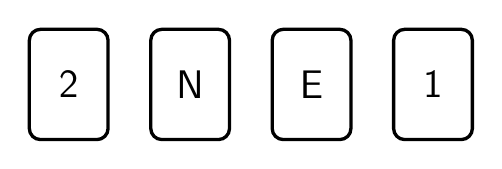
\begin{tikzpicture}[
      cardnode/.style={
        rectangle,
        minimum width=10mm,
        minimum height=14mm,
        align=center,
        rounded corners,
        font = {\Large\sffamily},
        very thick,
      },
      node distance=5mm,
      ]

      \node[cardnode, draw] (1) {2};
      \node[cardnode, draw, right = of 1] (2) {N};
      \node[cardnode, draw, right = of 2] (3) {E};
      \node[cardnode, draw, right = of 3] (4) {1};
    \end{tikzpicture}
    \caption{A selection task}
    \label{fig:sectionTask}
  \end{figure}

  \citeauthor{Wason:1966aa} observes the results are consistent with the following hypothesis:%
  \footnote{
    \citeauthor{Wason:1966aa} does not provide a detailed summary of the results.
    However, \citeauthor{Johnson-Laird:1969aa} detail results of \emph{twenty four} University College London students!
    Specifically, 19 of the 24 responded as excepted given \citeauthor{Wason:1966aa}'s hypothesis.
    (\citeyear[369--370]{Johnson-Laird:1969aa}).
  }
  \begin{quote}
    Subjects assume implicitly that a conditional statement has, not two truth values, but three: true, false and `irrelevant'.
    Vowels with even numbers verify, vowels with odd numbers falsify and consonants with any number are irrelevant.%
    \mbox{ }\hfill\mbox{(\citeyear[146]{Wason:1966aa})}
  \end{quote}
\end{note}

\begin{note}
  Selection tasks may be understood in connexion with \autoref{idea:tC}.
  In particular:
  %
  \begin{itemize}
  \item
    The relevant \tocN{} \(T\) is `reasoning via the material conditional'.%
    \footnote{
      \citeauthor{Wason:1966aa}'s hypothesis concerns a conditional statement having two truth values, but does not specify what these truth values are.
      Still, it is clear by inspection that these are the truth values of the material conditional.
    }
  \item
    The collection of possible events \(\mathcal{E}\) of interest contains selection tasks, plausibly taken under close to ideal circumstances.
    And,
  \item
    The collection of \prop{0}-\val{0}-\pool{0} pairings \(\mathcal{X}\) contains \prop{0}-\val{0}-\pool{0} pairings which capture appropriate \evalN{1} of what do.
    We specify these with a variable `\(C\)' to represent the relevant card:
    %
    \begin{center}
      \begin{tabular}{R{.40\textwidth} L{.40\textwidth}}
        \prop{2}-\val{0} pair & \prop{2}-\val{0} pairs in \pool{0} \\
        \hline
        \pv{C\propI{ needs to be turned over}}{\valI{True}} & \pv{C\propI{ has a vowel}}{\valI{True}} \\
        \pv{C\propI{ needs to be turned over}}{\valI{True}} & \pv{C\propI{ has an odd number}}{\valI{True}} \\
        \pv{C\propI{ needs to be turned over}}{\valI{False}} & \pv{C\propI{ has consonant}}{\valI{True}} \\
        \pv{C\propI{ needs to be turned over}}{\valI{False}} & \pv{C\propI{ has an even number}}{\valI{True}} \\
      \end{tabular}
    \end{center}
  \end{itemize}
  %
  As a consequence, \(\ed{}\) is an event when an agent is \tC{} some \prop{0}-\val{0} pair from some \pool{} by reasoning via the material conditional only if the agent would succeed at a selection task.

  \citeauthor{Wason:1966aa} observes most subjects do not succeed at selection tasks.
  Hence, \citeauthor{Wason:1966aa} suggests that subjects do not --- in general --- reason via the material conditional.
\end{note}


\begin{note}
  There is a important subtlety to this construction.
  Subjects clearly do reason in line with the material conditional.
  For example, various definitions and ideas (including \autoref{idea:tC}) in this document are given with an implicit expectation that any instance \emph{if} \dots \emph{then} \dots construction is understood in line with the material conditional.

  Hence, our reconstruction of \citeauthor{Wason:1966aa} does not state that subjects do not reason with the material conditional.
  Instead, the relevant \torN{} is intended to capture the idea that \emph{in general} subjects reason with conditionals via the material conditional.
  Rejecting that subjects `in general' reason with conditionals via the material conditional is compatible with subjects \emph{sometimes} reasoning with the material conditional.

  Specifying the relevant \torN{} is difficult.
  We understand there to be a difference between `reasoning via the material conditional' and `reasoning via the material conditional when implicitly or explicitly called on by the situation'.
  And, likewise, \citeauthor{Wason:1966aa}'s hypothesis of three truth values does not single out any particular \torN{}, as \citeauthor{Wason:1966aa} does not give a complete account of the truth values.

  Still, various other observations may be seen to parallel to our treatment of selection tasks via \autoref{idea:tC}.
  In particular, consider \citeauthor{Harman:1984aa}'s (\citeyear{Harman:1984aa,Harman:1986ux}) arguments against a strong connexion between logical principles and principles of belief revision.
  \citeauthor{Harman:1984aa} summarises:
  %
  \begin{quote}
    Logical principles are not directly rules of belief revision.
    [\dots]
    Logical principles hold universally, without exception, whereas the corresponding principles of belief revision would be at best prima facie principles, which do not always hold.%
    \mbox{ }\hfill\mbox{(\citeyear[107--108]{Harman:1984aa})}
  \end{quote}
    %
  Likewise, consider the \citeauthor{Allais:1979aa} paradox (\cite{Allais:1979aa}),
  the Ellsberg paradox (\cite{Ellsberg:1961aa}), \citeauthor{Makinson:1965aa}'s Paradox of the Preface (\citeyear{Makinson:1965aa}), \citeauthor{Kyburg:1997aa}'s Lottery Paradox (\citeyear{Kyburg:1997aa}), \citeauthor{Quinn:1990aa}'s  puzzle of the self-torturer (\citeyear{Quinn:1990aa}), \citeauthor{Bratman:1981aa}'s arguments against the desire-belief model of practical reasoning (\citeyear{Bratman:1981aa,Bratman:1987aa}), and so on.

  Common to each observation mentioned is the idea that an agent failing to conclude something shows that other instances of the agent's reasoning does not have some general characteristic.
\end{note}


% \paragraph*{Rules}

% \begin{note}
%   Selection tasks are events which happen, and \citeauthor{Wason:1966aa}'s hypothesis is that people \emph{in general} do not do not reason about conditionals using only \valI{True} and \valI{False}.
%   However, the events the law of \autoref{idea:tC} quantifies over need not happen, and the event at issue may be a single event.
% \end{note}

% \begin{note}
%   \begin{scenario}[Addition]%
%     \label{illu:quus}%
%     An agent is given pairs of numbers \(x\) and \(y\) and asked to respond with \(x + y\).
%     The table below represents the event as the agent responds to the pairs.

%     \medskip
%     \hspace{2.8em}%
%     \(
%       \begin{array}{ccccccc}
%       x & 3 & 54 & 21 & 3 & 17 & 0 \\
%       y & 7 & 32 & 64 & 2 & 25 & 6 \\
%       \hline
%       \text{Response} & 10 & 86 & 85 & 5 & 42 & 6 \\
%     \end{array}
%     \)
%     \medskip

%     \noindent%
%     The agent is distracted.
%     However, if the agent had not been distracted, they would have continued as follows:

%     \medskip
%     \hfill%
%     \(
%     \begin{array}{ccccc}
%       \cdots & 8 & 68 & 21 & 58 \\
%       \cdots & 92 & 57 & 23 & 92 \\
%       \hline
%       \cdots & 100 & 5 & 44 & 5 \\
%     \end{array}
%     \)%
%     \hspace{2.8em}%
%     \mbox{ }%
%     \newline%
%   \end{scenario}

%   \noindent%
%   It seems the agent was not reasoning by addition.%
%   \footnote{
%     Rather, it seems the agent was reasoning by quaddition, following \citeauthor{Kripke:1982aa}'s (\citeyear{Kripke:1982aa}) definition of `quss':
%     \begin{align*}
%       x \text{ quss y} &= x \text{ plus } y, \text{ if } x,y < 57 \\
%                        &= 5 \phantom{pl if x,,,} \text{ otherwise }
%     \end{align*}
%     \vspace{-\baselineskip}
%   }

%   For, consider the counterfactual event.
%   The agent concluded \pv{\propI{x + y is 5}}{\valI{True}} from some \pool{} containing \pv{\propI{x is 68}}{\valI{True}} and \pv{\propI{y is 57}}{\valI{True}}.
%   Hence, it seems the agent was not concluding \pv{\propI{x + y is 125}}{\valI{True}}.

%   Further, though the counterfactual event suggests the agent was not reasoning by addition, it is less clear that the agent never reasons by addition.
%   The agent's interpretation of `\(+\)' as something other than `plus' may be no different from interpreting `\(A \land B\)' as `\(A\) and \(B\)' rather than `the meet of sets \(A\) and \(B\)'.
% \end{note}


\paragraph*{Powers}

\begin{note}
  Selection tasks are events which happen and highlight an \agents{} reasoning is not of some particular type.
  However, our interest with \tCN{} primarily concerns events where the agent \emph{is} \tCV{} by some type, and \autoref{idea:tC} suggests the agent would make some conclusion if some possible event were to happen.
\end{note}

\begin{note}
  \begin{scenario}[Powerful multiplication]%
    \label{illu:tR:powers}%
    A student has been studying algebra and has just been introduced to the rule of multiplication for powers (\(a^{n} \cdot a^{m} = a^{n + m}\)).

    At hand are a handful of exercises (from \cite[32]{Gelfand:1993aa}):
    %
    \begin{quote}
      \begin{enumerate}[label=(\alph*), ref=(\alph*)]
      \item
        \label{mfp:a}
        You know that \(2^{1001} \cdot 2^{n} = 2^{2000}\).
        What is \(n\)?
      \item
        \label{mfp:b}
        You know that \(2^{1001} \cdot 2^{n} = \sfrac{1}{4}\).
        What is \(n\)?
      \item
        \label{mfp:c}
        Which is bigger: \(10^{-3}\) or \(2^{-10}\)?
      \item
        \label{mfp:d}
        You know that \(\sfrac{2^{1000}}{2^{n}} = 2^{501}\).
        What is \(n\)?
      \item
        \label{mfp:e}
        You know that \(\sfrac{2^{1000}}{2^{n}} = \sfrac{1}{16}\).
        What is \(n\)?
      \item
        \label{mfp:f}
        You know that \(4^{100} = 2^{n}\).
        What is \(n\)?
      \item
        \label{mfp:g}
        You know that \(2^{100} \cdot 3^{100} = a^{100}\).
        What is \(a\)?
      \item
        \label{mfp:h}
        You know that \((2^{10})^{15} = 2^{n}\).
        What is \(n\)?
      \end{enumerate}
    \end{quote}
    %
    The student starts work on exercise~\ref{mfp:f}, and is concluding \(\pv{n\propI{ is }200}{\valI{True}}\).
  \end{scenario}

  \noindent%
  Intuitively, the student is reasoning with an understanding of multiplication for powers.

  Further, it seems the agent is concluding \pv{\propI{n is 200}}{\valI{True}} by an understanding of multiplication for powers \emph{only if} the agent would be concluding \pv{\propI{a is 6}}{\valI{True}} from \pv{\propM{2^{100} \cdot 3^{100} = a^{100}}}{\valI{True}} were the agent to abandon \ref{mfp:g} and work on~\ref{mfp:f}.

  Indeed, it is plausible exercises \ref{mfp:a} through to \ref{mfp:h} were chosen by \citeauthor{Gelfand:1993aa} to test basic competence with multiplication for powers.
  Hence, if the agent would fail to be concluding \pv{\propI{a is 6}}{\valI{True}} from \pv{\propM{2^{100} \cdot 3^{100} = a^{100}}}{\valI{True}} when working on~\ref{mfp:f}, then it seems the agent does not have an adequate understanding of multiplication for powers to be concluding \emph{by} an understanding of multiplication for powers.%
  \footnote{
    This may be resisted.
    For example, exercises~\ref{mfp:b},~\ref{mfp:d}, and~\ref{mfp:e} all involve fractions.
    And, the agent may be shaky on fractions, but good with multiplication by powers.
    Hence, the relevant collection \prop{0}-\val{0}-\pool{0} pairings \(\mathcal{X}\) may only include \prop{0}-\val{0}-\pool{0} pairings which correspond to exercises \ref{mfp:a},  \ref{mfp:c},  \ref{mfp:f},  \ref{mfp:g}, and \ref{mfp:h}.

    For broader motivation for such restrictions, consider \citeauthor{Chomsky:2015aa}'s distinction between competence and performance.
    %
    \begin{quote}
      Arithmetical competence yields the correct number z for every pair~(x,~y) under addition or multiplication.
      But only a small finite subpart of arithmetical competence can be exhibited without external aids (by calculating in one's head).
      Obviously, that fact does not imply that arithmetical competence is correspondingly limited.%
      \mbox{ }\hfill\mbox{(\citeyear[xii]{Chomsky:2015aa})}
    \end{quote}
  }
\end{note}



\section{\tC{2} and \fc{1}}
\label{cha:typical:tCDef}


\begin{note}
  \autoref{sec:idea} introduced the idea of an agent \tCV{} (\autoref{idea:tC}).
  The present section links an agent \tCV{} to the idea of \fc{1}.
\end{note}

\begin{note}
  \begin{proposition}[\typeAdj{2} \fc{1}]%
    \label{prop:tCV-fc}%
    \vspace{-\baselineskip}
    \begin{itenum}
    \item[\emph{If}:]
      Conditions \ref{prop:tCV-fc:tC} and \ref{prop:tCV-fc:e} hold:
      \begin{enumerate}[label=\arabic*., ref=\arabic*]
      \item
        \label{prop:tCV-fc:tC}
        \(\ed{}\) is an event in which \vAgent{} is \tCV{} \(\pv{\phi}{v}\) from \(\Phi\) by \torNa{} \(T\).
      \item
        \label{prop:tCV-fc:e}
        There is some partition of \(\ed{}\) into sub-events \(\edn{1}, \dots, \edn{k}\) such that for some event \(\edn{i}\) in the partition:
        \begin{itemize}
        \item
          There is some possible event \(\edn{\sharp}\) in \(\mathcal{E}\) and \prop{0}-\val{0}-\pool{0} pairing \(\pvp{\psi}{v'}{\Psi}\) in \(\mathcal{X}\) such that:
          \begin{enumerate}[label=\alph*., ref=\theenumi\alph*]
          \item
            \label{prop:tCV-fc:e:act:i}
            \(\edn{\sharp}\) is the result of an action \(a\) done by \vAgent{} in \(\ed{i}\)
          \item
            \label{prop:tCV-fc:e:act:ii}
            \vAgent{} \evals{} \(\psi'\) as having value \(v''\) prior to doing \(a\), for each \prop{0}-\val{0} pair \(\pv{\psi'}{v''}\) in \(\Psi\).
          \end{enumerate}
        \end{itemize}
      \end{enumerate}
    \item[\emph{Then}:]
      There is some \prop{0}-\val{0}-\pool{0} pairing \(\pvp{\psi}{v'}{\Psi}\) such that:
      \begin{itemize}
      \item
        \(\pv{\psi}{v'}\) is a \fc{0} from \(\Psi\) for \vAgent{} throughout \(\ed{i}\).
      \end{itemize}
    \end{itenum}
    \vspace{-\baselineskip}
  \end{proposition}

  \noindent%
  \autoref{prop:tCV-fc} considers a \scen{0} in which an agent is \tCV{} and the collection of possible events and \prop{0}-\val{0}-\pool{0} pair satisfies conditions.

  First condition.
  \tCV{} a collection of possible events.
  In some cases, possible events correspond to result of the agent doing some action.

  As agent is \tCV{}, then for each event, \prop{0}-\val{0}-\pool{0} pairing such that the agent is concluding.
  Second condition, agent does not require novel information after action is done to conclude.

  For example, consider \autoref{illu:tR:powers}.
  Agent is concluding \pv{\propI{n is 200}}{\valI{True}} by an understanding of multiplication for powers \emph{only if} the agent would be concluding \pv{\propI{a is 6}}{\valI{True}} from \pv{\propM{2^{100} \cdot 3^{100} = a^{100}}}{\valI{True}} were the agent to abandon \ref{mfp:g} and work on~\ref{mfp:f}.
  So, we have some collection of events, result of action.
  And, second condition is satisfied.
\end{note}

\begin{note}
  The full argument for \autoref{prop:tCV-fc}, though merely amounts to generalising the above observation by citing the relevant definitions.

  \begin{argument}{prop:tCV-fc}
    Suppose conditions \ref{prop:tCV-fc:tC} and \ref{prop:tCV-fc:e} hold.

    By Condition~\ref{prop:tCV-fc:tC}, \(\ed{}\) is an event in which \vAgent{} is \tCV{} \(\pv{\phi}{v}\) from \(\Phi\) by \torNa{} \(T\).
    So, by \autoref{idea:tC} there is some collections \(\mathcal{E}\) of events and \(\mathcal{X}\) of \prop{0}-\val{0}-\pool{0}~pairings such that:
    %
    \begin{itemize}[noitemsep]
    \item
      For every event \(\ed{\prime}\), there is some \prop{0}-\val{} pair \(\pv{\psi}{v'}\) and \pool{0} \(\Psi\) in \(\mathcal{X}\) such that:
      \begin{itenum}[noitemsep]
      \item[\emph{If}:]
        \(\ed{\prime}\) is in the collection of events \(\mathcal{E}\).
      \item[\emph{Then}:]
        \(\ed{\prime}\) is an event in which \vAgent{} is concluding \(\pv{\psi}{v'}\) from \(\Psi\).
      \end{itenum}
    \end{itemize}
    %
    Further, Condition~\ref{prop:tCV-fc:e} concerns a sub-event \(\edn{i}\) of some partition of \(\ed{}\) into sub-events \(\edn{1}, \dots, \edn{k}\).
    In particular, there is some possible event \(\edn{\sharp}\) in \(\mathcal{E}\) and \prop{0}-\val{0}-\pool{0} pairing \(\pvp{\psi}{v'}{\Psi}\) in \(\mathcal{X}\) such that:
    \begin{enumerate}[label=\alph*., ref=\theenumi\alph*]
    \item
      \(\edn{\sharp}\) is the result of an action \(a\) done by the agent in \(\ed{}\).
    \item
      The agent \evals{} \(\psi'\) as having value \(v''\) prior to doing \(a\), for each \prop{0}-\val{0} pair \(\pv{\psi'}{v''}\) in \(\Psi\).
    \end{enumerate}
    By Condition \ref{prop:tCV-fc:e:act:i} and \autoref{idea:tC}, it follows that the agent is concluding \(\pv{\psi}{v'}\) from \(\Psi\) in \(\edn{\sharp}\).

    Now, \(\edn{i}\) is trivially a partition of \(\edn{i}\) into sub-events.
    And, as just observed there is some description \(d_{i}\) such that \(\ed{i}\) is an event in which the agent may do some action \(a_{i}\) where:
    %
    \begin{enumerate}[label=\Alph*., ref=\Alph*, series=tCVFCArg]
    \item
      The event \(\ed{i+}\) in which the agent does \(a_{i}\) is an event in which the agent is concluding \(\pv{\psi}{v'}\) from \(\Psi\).
    \end{enumerate}
    %
    Further, by Condition~\ref{prop:tCV-fc:e:act:ii}:
    %
    \begin{enumerate}[label=\Alph*., ref=\Alph*, resume*=tCVFCArg]
    \item
      The agent \evals{} \(\psi'\) as having value \(v''\) prior to doing \(a_{i}\), for each \prop{0}-\val{0} pair \(\pv{\psi'}{v''}\) in \(\Psi\).
    \end{enumerate}
    %
    Hence, the definition of \(\pv{\phi}{v}\) being a \fc{0} from \(\Psi\) throughout \(\ed{i}\) is satisfied (cf.~\autoref{def:fc}, \autopageref{def:fc}).
  \end{argument}
\end{note}


\section{An \illu{0}}


\begin{note}
  To close this chapter we offer a final \illu{0} of \tCV{}, though this time with a focus on \fc{1} given \autoref{prop:tCV-fc}.
\end{note}


\begin{note}
  \phantlabel{squish-elimination-proof}

  \begin{scenario}[Squish elimination]%
    \label{scen:squish}%
    Some time ago the agent showed \sqE{} is sound.

    It is now late morning on a sunny day.
    The agent ate a good breakfast, and drank some nice coffee and does the following syntactic proof:
    %
    \begin{center}
      \begin{fitch}
        \phantlabel{illu:sP:1}\fa (P \rightarrow Q) \rightarrow P \\
        \phantlabel{illu:sP:2}\fj R \\
        \phantlabel{illu:sP:3}\fa P & \sqE{}:\hyperref[illu:sP:1]{1} \\
        \phantlabel{illu:sP:4}\fa P \land R & \(\land\)\textbf{Intro:} \hyperref[illu:sP:2]{2},\hyperref[illu:sP:3]{3}
      \end{fitch}
    \end{center}
    %
    The agent concludes \((P \rightarrow Q) \rightarrow P, R \vdash P \land R\).
  \end{scenario}

  \noindent%
  Intuitively, agent \tCV{} \((P \rightarrow Q) \rightarrow P, R \vdash P \land R\) from some \pool{} which captures the \agents{} understanding of the relevant Fitch-style proof system.
  And, as the agent is \tCV{}, some \torNa{} captures the \agents{} understanding of the relevant Fitch-style proof system.
\end{note}


\begin{note}
  Still, in \autoref{scen:squish} the agent uses the non-standard \sqE{} rule.
  Specifically:

  \begin{definition}[\sqE{}]%
    \label{def:sque}%
    \sqE{} is the following rule:
    \begin{center}
      \begin{fitch}
        \ftag{\text{\scriptsize \emph{i}}}{\fa (\phi \rightarrow \psi) \rightarrow \phi} \\
        \ftag{\text{\scriptsize }}{\fa \vdots } \\
        \ftag{\text{\scriptsize \emph{j}}}{\fa \phi } & \sqE{}:\emph{i} \\
      \end{fitch}
    \end{center}
  \end{definition}

  \noindent%
  By stipulation, the agent has proved \sqE{} is sound.
  And, \sqE{} is indeed sound.%
  \footnote{
    \label{prop:sqE-sound}
    Rather than prove \sqE{} is sound (which would require a detailed statement of the proof system in question), we show that the key corresponding semantic entailment holds:

    Let \(v\) be an arbitrary (truth-functional) valuation, and assume \(v((\phi \rightarrow \psi) \rightarrow \phi) = \valI{True}\).
    Further, assume for contradiction \(v(\phi) = \valI{False}\).

    As \(v(\phi) = \valI{False}\), it immediately follows that \(v(\phi \rightarrow \psi) = \valI{True}\).
    Therefore, by the first assumption, it must be the case that \(v(\phi) = \valI{True}\).
    This contradictions the second assumption.
  }

  Still, \((P \rightarrow Q) \rightarrow P, R \vdash P \land R\) may be logic soup.
  The agent has proved \sqE{} is sound.
  Though, no guarantee that the \agents{} recollection of \sqE{} is tied to their understanding of the relevant Fitch-style proof system.

  In parallel to failing to identify correct cards, or failing solve exercise, something wrong.
\end{note}


\begin{note}
  Further, the proof of the soundness of \sqE{} is fairly straightforward.
  Hence, if the agent is \tCV{}, some action such that concluding \sqE{} is sound.%
  \footnote{
    Two options.
    Either directly show \sqE{} follows from the \agents{} understanding of the proof system via constructing a meta-proof of \sqE{} or indirectly show \sqE{} follows by providing a semantic argument and combine with completeness result.
    If neither direct or indirect, then the \agents{} use of \sqE{} does not follow from the \agents{} understanding of relevant Fitch-style proof system.
  }
  From \autoref{prop:tCV-fc}, \fc{}.%
  \footnote{
    Further, \sqaE{}, \sqoE{}, and \sqeE{} are all unsound.
    Respectively, the following rules:

    \mbox{ }\hfill
    \begin{minipage}[c]{0.25\textwidth}\vspace{0pt}
      \begin{fitch}
        \ftag{\text{\scriptsize \emph{i}}}{\fa \phi \rightarrow (\psi \rightarrow \phi)} \\
        \ftag{\text{\scriptsize }}{\fa \vdots } \\
        \ftag{\text{\scriptsize \emph{j}}}{\fa \phi } \\
      \end{fitch}
    \end{minipage}
    \hfill
    \begin{minipage}[c]{0.25\textwidth}\vspace{0pt}
      \begin{fitch}
        \ftag{\text{\scriptsize \emph{i}}}{\fa \psi \rightarrow (\phi \rightarrow \psi)} \\
        \ftag{\text{\scriptsize }}{\fa \vdots } \\
        \ftag{\text{\scriptsize \emph{j}}}{\fa \phi } \\
      \end{fitch}
    \end{minipage}
    \hfill
    \begin{minipage}[c]{0.25\textwidth}\vspace{0pt}
    \begin{fitch}
        \ftag{\text{\scriptsize \emph{i}}}{\fa (\psi \rightarrow \phi) \rightarrow \psi} \\
        \ftag{\text{\scriptsize }}{\fa \vdots } \\
        \ftag{\text{\scriptsize \emph{j}}}{\fa \phi } \\
      \end{fitch}
    \end{minipage}
    \hfill\mbox{ }
}
\end{note}


\begin{note}
  Does not require that the agent (re)proves \sqE{} is sound.
  At issue is that the agent has the option.
  Likewise, this does not state this is enough to state the agent is \tCV{}.
  \autoref{idea:tC} is a partial definition.
\end{note}

\section*{Summary}

\begin{note}
  \tCN{2}.

  Extension account of \torN{}.
  Due to abstracting over theories.

  Then, necessary condition on \tC{}.
\end{note}

\begin{note}
  Only motivated \tC{} by intuition.
  Have not argued that this intuition is correct.
  Key piece, and intuitive.
\end{note}




% \section[\citeauthor{Carroll:1895uj}]{\citeauthor{Carroll:1895uj}\hfill(Optional)}

% \nocite{Black:1951aa}

% \begin{note}
%   The point here is that with Carroll, generality that goes beyond any single instance.
%   Must apply to all instances, to be valid.
%   But, cannot hope to cover all instances in a single move.
% \end{note}

% \begin{note}
%   A difficulty found on a reading of \citeauthor{Carroll:1895uj}'s \citetitle{Carroll:1895uj}.
% \end{note}

% \begin{note}
%   \begin{quote}
%     ``Plenty of blank leaves, I see!'' the Tortoise cheerily remarked.
%     ``We shall need them \emph{all}!''
%     (Achilles shuddered.)
%     ``Now write as I dictate:---

%     \begin{enumerate}[label=(\emph{\Alph*}), ref=\emph{\Alph*}]
%     \item
%       \label{AatT:a}
%       Things that are equal to the same are equal to each other.
%     \item
%       \label{AatT:b}
%       The two sides of this Triangle are things that are equal to the same.
%     \item
%       \label{AatT:c}
%       If~\ref{AatT:a} and~\ref{AatT:b} are true,~\ref{AatT:z} must be true.
%       \setcounter{enumi}{25}
%     \item
%       \label{AatT:z}
%       The two sides of this Triangle are equal to each other.''
%     \end{enumerate}

%     ``You should call it~\ref{AatT:d}, not~\ref{AatT:z},'' said Achilles.
%     ``It comes \emph{next} to the other three.
%     If you accept~\ref{AatT:a} and~\ref{AatT:b} and~\ref{AatT:c}, you \emph{must} accept~\ref{AatT:z}.''

%     ``And why \emph{must} I?''

%     ``Because it follows \emph{logically} from them.
%     If~\ref{AatT:a} and~\ref{AatT:b} and~\ref{AatT:c} are true,~\ref{AatT:z} \emph{must} be true.
%     You don't dispute \emph{that}, I imagine?''

%     ``If~\ref{AatT:a} and~\ref{AatT:b} and~\ref{AatT:c} are true,~\ref{AatT:z} \emph{must} be true,'' the Tortoise thoughtfully repeated.
%     ``That's \emph{another} Hypothetical, isn't it?
%     And, if I failed to see its truth, I might accept~\ref{AatT:a} and~\ref{AatT:b} and~\ref{AatT:c}, and \emph{still} not accept~\ref{AatT:z}, mightn't I ?''

%     \mbox{}\hfill\(\vdots\)\hfill\mbox{}

%     ``Then Logic would take you by the throat, and force you to do it!''
%     Achilles triumphantly replied.
%     ``Logic would tell you 'You ca'n't help yourself.''%
%     \mbox{ }\hfill\mbox{(\citeyear[279--280]{Carroll:1895uj})}
%   \end{quote}

%   The Tortoise has written down three premises,~\ref{AatT:a},~\ref{AatT:b}, and~\ref{AatT:c}.
%   Achilles holds that~\ref{AatT:z} follows from~\ref{AatT:a},~\ref{AatT:b}, and~\ref{AatT:c}.
%   The Tortoise observes they have the possibility of refraining to accept~\ref{AatT:z} follows from~\ref{AatT:a},~\ref{AatT:b}, and~\ref{AatT:c}.
%   And (initially), the Tortoise does not accept~\ref{AatT:z} follows from~\ref{AatT:a},~\ref{AatT:b}, and~\ref{AatT:c}.
%   Achilles requests the Tortoise accepts that~\ref{AatT:z} follows from~\ref{AatT:a},~\ref{AatT:b}, and~\ref{AatT:c}, and the Tortoise complies.
%   Specifically, the Tortoise grants:

%   \begin{quote}
%     \begin{enumerate}[label=(\emph{\Alph*}), ref=\emph{\Alph*}]
%       \setcounter{enumi}{3}
%     \item
%       \label{AatT:d}
%       If~\ref{AatT:a} and~\ref{AatT:b} and~\ref{AatT:c} are true,~\ref{AatT:z} must be true.%
%       \mbox{ }\hfill\mbox{(\citeyear[279]{Carroll:1895uj})}
%     \end{enumerate}
%   \end{quote}

%   But, does not accept~\ref{AatT:z} follows from~\ref{AatT:a},~\ref{AatT:b},~\ref{AatT:c}, and~\ref{AatT:d}.
% \end{note}

% \begin{note}
%   Modus ponens.

%   \begin{quote}
%     From \(\phi\) and \emph{if} \(\phi\) then \(\psi\), infer \(\psi\).
%   \end{quote}

%   Modus ponens is general.
%   For \emph{any} \(\phi\), \(\psi\).

%   Now, there is a difference between \emph{modus ponens} and conditional.

%   However, take any instance.
%   Then, if \(P\), \(P \rightarrow Q\), \(Q\) must be true.
%   But, then this means that the conditional is true.

%   Consequence of the deduction theorem.

%   Likewise, deduction theorem goes the other way.

%   However, going from \(P\), \(P \rightarrow Q\) to \(Q\) need not be an instance of \emph{modus ponens}.
% \end{note}

% \begin{note}
%   Well, this is a headache.
%   \citeauthor{Carroll:1895uj} is talking about a specific A, B, and Z.
%   There is no clear generality.
% \end{note}

% \begin{note}
%   So, consider at issue is modus ponens.
%   For any specific instance accept, there is a further instance.
%   For, \(A, (A \rightarrow B) \vDash B\).
%   Then, \(\vDash (A \land (A \rightarrow B) \rightarrow B)\).
%   However, now, \(A \land (A \rightarrow B), (A \land (A \rightarrow B) \rightarrow B) \vDash B\).
%   And, so on.

%   The general pattern, get conditional, but then this gives a new instance of modus ponens, which must be true in order for modus ponens to be valid rule of inference.

%   \citeauthor{Carroll:1895uj}, by contrast, starts with \(A \vDash B\).
%   This is different.
%   However, rather than focusing on a single rule of inference, the puzzle turns on what validity amounts to.

%   Validity is a general thing, with specific instances.
%   However, grant any particular instance of validity without employing validity in general.
% \end{note}

% \begin{note}
%   \begin{quote}
%     My paradox \dots turns on the fact that, in a Hypothetical, the \emph{truth} of the Protasis, the \emph{truth} of the Apodosis, and the \emph{validity of the sequence}, are 3 distinct Propositions.

%     \mbox{}\hfill\(\vdots\)\hfill\mbox{}

%     Suppose I say ``I grant~\ref{AatT:a} and~\ref{AatT:b} and~\ref{AatT:c}, but I do \emph{not} grant that I am thereby \emph{obliged} to grant~\ref{AatT:z}.''
%     Surely, my granting~\ref{AatT:z} must \emph{wait} until I have been made to see the validity of this sequence: i.e.\ in order to grant~\ref{AatT:z}, I must grant~\ref{AatT:a},~\ref{AatT:b},~\ref{AatT:c}, and~\ref{AatT:d}! And so on.%
%     \mbox{ }\hfill\mbox{(\citeyear[472]{Carroll:1977wl})}
%   \end{quote}

%   My interpretation of the point \citeauthor{Carroll:1895uj} makes in this passage is that the truth of A B and the truth of C is distinct from the validity of A B C.
%   Granting is substantial, not merely moving.
%   But, in order to grant, this means granting all other cases.

%   So, the paradox is that, on the one hand, don't need validity for any specific true things.
%   But, on the other hand, only of interest if via validity.

%   The Tortoise is slowly working through each instance, but this has no hope of getting the Tortoise to general validity.
%   So, how does the Tortoise ever make it there?
% \end{note}

% \begin{note}
%   This point differs from received interpretation.

%   \citeauthor{Wieland:2013vf} (\citeyear{Wieland:2013vf}) characterises the general understanding of \textcite{Carroll:1895uj} in terms of two lessons:
%   \begin{quote}
%     [T]he negative lesson is that if you add ever more premises to an argument \dots, then you will never demonstrate that its conclusion follows logically.\newline
%     \mbox{ }\hfill\mbox{(\citeyear[984]{Wieland:2013vf})}
%   \end{quote}

%   Parallel, static answers, still option for concluding otherwise.

%   \begin{quote}
%     [T]he positive lesson is that rules of inference, rather than premises of the form `if premises such and such are true, then the conclusion is true', will do the job.\newline
%     \mbox{ }\hfill\mbox{(\citeyear[984]{Wieland:2013vf})}
%   \end{quote}

%   \begin{quote}
%     [\citeauthor{Carroll:1895uj}] simply lacked any distinct conception of a deduction as opposed to the assertion (``granting'' of) a hypothetical proposition.
%     \dots
%     Any attempt by Carroll to tackle the question of inference was bound to begin in confusion and end in constipation-all those premises piling up, but no motion.
%   \end{quote}
% \end{note}

% \paragraph{The Dichotomy}

% \begin{note}
%   Achilles and the Tortoise, Zeno's argument.

%   Surely, right?

%   Two ways to understand.
%   Does the Tortoise move at all, or does the Tortoise arrive at the end?
%   I mean, as formulated by Zeno, it's about catching up, no matter how much one moves.

%   It is different from Zeno's Dichotomy paradox.


%   If so, then we should expect the Tortoise to be making some movement.
%   Adding rules of inference is of no help, because the problem is not movement, it's about how to move so much in a single step.
% \end{note}

% \begin{note}
%   \color{red}
%   Something about logic forcing.
%   The Tortoise hasn't arrived.

%   Nothing hangs on validity.
%   Same issue with testimony.
%   `A'.
%   Why?
%   Testified A, so A.
%   Okay, but another instance of testimony.
%   Testified(Testified A, so A), so Testified A, so A.
% \end{note}

% \begin{note}
%   \begin{quote}
%     But if we who wish to represent his belief in Q as based on P are to write in our notebook everything his having that belief on that basis consists in then when we have written only P and Q we will not have written enough.
%     Someone can believe P and believe Q and still not believe Q on the basis of P whatever the relations between the propositions P and Q happen to be.
%     He might believe Q for some reason completely unconnected with P, or perhaps for no reason at all (if that is possible).%
%     \mbox{ }\hfill\mbox{(\citeyear[185]{Stroud:1979aa})}
%   \end{quote}
%   However, the moral drawn is narrow
%   \begin{quote}
%     The moral is that for every proposition or set of propositions the belief or acceptance of which is involved in someone's believing one proposition on the basis of another there must be something else, not simply a further proposition accepted, that is responsible for the one belief's being based on the other.%
%     \mbox{ }\hfill\mbox{(\citeyear[187]{Stroud:1979aa})}
%   \end{quote}

%   Even if we grant each individual is \ros{}, rather than an instance of the material conditional, \emph{logic} hasn't done anything.
% \end{note}

% \paragraph{General and specific: Contrast}

% \begin{note}
%   Use \citeauthor{Carroll:1895uj} to illustrate this point.

%   However, given the worry, various other things may be understood this way.

%   Hume, constant conjunction.
%   Part of the problem is identifying cause.
%   We get the famous line about observing.
%   However, Hume goes on.
%   It's not only no observation, but no generality.

%   Right, so more narrow than Hume.
%   Because, with Hume, at issue is whether we have grounds for this general thing.
%   With Carroll, it's whether we even really get to the general thing.
% \end{note}

% \begin{note}
%   \begin{quote}
%     Let me ask this: what has the expression of a rule—say a sign-post—got to do with my actions?
%     What sort of connexion is there here?%
%     ---%
%     Well, perhaps this one:
%     I have been trained to react to this sign in a particular way, and now I do so react to it.

%     But that is only to give a causal connexion; to tell how it has come about that we now go by the sign-post; not what this going-by-the sign really consists in.
%     On the contrary; I have further indicated that a person goes by a sign-post only in so far as there exists a regular use of sign-posts, a custom.%
%     \mbox{ }\hfill\mbox{(\citeyear[\S198]{Wittgenstein:1958aa})}
%   \end{quote}

%   Regular use of sign-posts, custom.

%   Ugh, this is ambiguous.
% \end{note}


% %
%   \(^{,}\)
%   \footnote{
%     \citeauthor{Hlobil:2014tq}'s ``Inferential Moorean Phenomenon'':
%   \begin{quote}
%     \begin{enumerate}
%     \item[(IMP)]
%       It is either impossible or seriously irrational to infer \emph{P} from \emph{Q} and to judge, at the same time, that the inference from \emph{Q} to \emph{P} is not a good inference.
%     \end{enumerate}
%     \dots
%     By the ``goodness'' of an inference I mean the feature that makes the relevant inference permissible. Thus, if the inference under consideration is an inductive inference, the relevant kind of goodness is not deductive validity.%
%     \mbox{ }\hfill\mbox{(\citeyear[\S1]{Hlobil:2014tq})}
%   \end{quote}
%   Though, this really isn't more basic given the interest in \tR{}.
%   For, the puzzle is what it is to `infer'.

%   Rationality isn't part of the picture.
%   And, this is a significant drawback of \citeauthor{Hlobil:2014tq}'s approach.
% }


% \subsection{Types and explanation}
% \label{cha:typical:sec:tor:bkgd}

% \begin{note}
%   There is a related, stronger claim, that generality derives from rule following.

%   For this, \citeauthor{Boghossian:2008vf}:

%   \begin{quote}
%     [O]ur internalization of general epistemic rules---like Modus Ponens and Induction---explain and rationalize why we form the beliefs that we form.
%     And that seems intuitively correct.

%     As in the case of our linguistic and conceptual abilities, our ability to form rational beliefs is \emph{productive}: on the basis of finite learning, we are able to form rational beliefs under a potential infinity of novel circumstances.
%     The only plausible explanation for this is that we have, somehow, internalized a rule that tells us, in some general way, what it would be rational to believe under varying epistemic circumstances.%
%     \mbox{ }\hfill\mbox{(\citeyear[483]{Boghossian:2008vf})}
%   \end{quote}

%   Strictly, \citeauthor{Boghossian:2008vf}, rules \textquote{represent our conception of how it would be most rational for a thinker to form beliefs under different epistemic circumstances} (\citeyear[473]{Boghossian:2008vf}).

%   The difference in approach is clearest with \citeauthor{Boghossian:2008vf}'s account of modus ponens:%
%   \footnote{
%     \citeauthor{Boghossian:2008vf} notes the rule is distinct from modus pones as found in textbooks.
%     Remarks: \textquote{It is actually quite mysterious what the logic textbook rule is supposed to be} (\citeyear[472,fn.2]{Boghossian:2008vf})
%     I don't think there is any mystery about the rule in most logic textbooks.
%     Instead, the mystery is the way in which logic relates to reasoning.
%     (Cf.~\cite{Harman:1986ux,MacFarlane:2004aa,Steinberger:2022aa}, etc.)
%     % Issue for the presentation.
%     % Literature is full of issues.
%     % The most well known, Gricean pragmatics.
%     % Though, also McGee, McFarlane, sweet conditonals, the miners paradox, etc.
%   }

%   \begin{quote}
%     (Modus Ponens):
%     If you are rationally permitted to believe both that \emph{p} and that `If \emph{p}, then \emph{q}', then, you are prima facie rationally permitted to believe that \emph{q}.%
%     \mbox{ }\hfill\mbox{(\citeyear[472]{Boghossian:2008vf})}
%   \end{quote}

%   Here, we have permissions.
%   What the agent is allowed to do.
%   However, this is distinct from what the agent does.
% \end{note}

% \begin{note}
%   \tR{} is distinct.
%   Whether came to \emph{q} from \emph{p} , if \emph{p} then \emph{q}.

%   Rationality is not part of our understanding.
%   Rather, generality.%
%   \footnote{
%     Observe, ~\cite{Kolodny:2005aa} is of no interest here.
%     Why be rational is distinct from whether there is some generality.
%   }
% \end{note}

% \begin{note}
%   Likewise, means-end reasoning is distinct from \citeauthor{Broome:2013aa}'s

%   \begin{quote}
%     \emph{End to Means Transmission}.
%     ((\emph{S} requires of \emph{N} that \emph{p}) \& necessarily \newline (\emph{p} \(\supset\) \emph{q}) \& \emph{q} is a means to \emph{p}) \(\supset\) (\emph{S} requires of \emph{N} that \emph{q}).%
%     \mbox{ }\hfill\mbox{(\citeyear[126]{Broome:2013aa})}
%   \end{quote}

%   \emph{S} is some source, such as morality.
%   \emph{N} is a person. (\citeyear[117]{Broome:2013aa})

%   Instead, the significantly weaker idea that the agent has reasoned from some end to a means to that end.
% \end{note}

% \begin{note}
%   On my understanding, this is, in part, the role of \citeauthor{Boghossian:2014aa}'s Taking Condition.

%   Way in which \dots

%   Indeed, \citeauthor{Boghossian:2014aa} highlights how condition allow to draw distinction between deductive and inductive.
%   With taking, get generality.

%   Indeed, \textcite{Boghossian:2014aa} is structured so that Taking is a generalisation of rule.
% \end{note}

% \begin{note}
%   However, \tor{} does not need to amount to a rule.
%   Rather, \tR{} only requires the rough phenomenon that \citeauthor{Boghossian:2008vf} argues rule following is the only plausible explanation of.%
%   \footnote{
%     Our interest with \tor{1} is independent of the worries about rule following raised by~\textcite{Kripke:1982aa}, to the extent that the worries raised by~\citeauthor{Kripke:1982aa} concern \emph{which} rule an agent is following, rather than \emph{whether} the agent is following a rule.
%     At interest is not whether the \tor{} corresponds to plus or quus, but whether the agent's reasoning is of some type.
%   }
% \end{note}

% \begin{note}
%   Same for modus ponens.

%   \citeauthor{Davies:2004aa} discussing~\textcite{Wright:2004aa} with respect to~\citeauthor{Moore:1959aa}'s proof of an external world (\citeyear{Moore:1959aa}):

%   \begin{quote}
%     Moore's argument can be set out as follows:
%     \begin{quote}
%       \begin{enumerate}[label=MOORE (\Roman*), ref=MOORE (\Roman*)]
%       \item
%         \label{MoorePoEW:1}
%         I am having an experience as of one hand [here] and another [here].
%       \item
%         \label{MoorePoEW:2}
%         I have hands.

%         If I have hands then an external world exists.
%       \end{enumerate}

%       Therefore:

%       \begin{enumerate}[label=MOORE (\Roman*), ref=MOORE (\Roman*), resume]
%       \item
%         \label{MoorePoEW:3}
%         An external world exists.
%       \end{enumerate}
%     \end{quote}

%     [\dots] the key question at this point in Wright's account is whether the support for~\ref{MoorePoEW:2} is transmitted to~\ref{MoorePoEW:3} across the modus ponens inference in which the conditional premise is supported by an elementary piece of philosophical theorising.\newline
%     \mbox{ }\hfill\mbox{(\citeyear[215]{Davies:2004aa})}
%   \end{quote}
% \end{note}



\begin{note}
  Or, whether properly based.%
  \footnote{
    \citeauthor{Schaffer:2010vq}'s (\citeyear{Schaffer:2010vq}) Debasing demon.

    The debasing demon \textquote{throws her victims into the belief state on an improper basis, while leaving them with the impression as if they had proceeded properly}. (\citeyear[231]{Schaffer:2010vq})

    (However, see \textcite{Bondy:2018tk} for ways in which the \citeauthor{Schaffer:2010vq}'s demon fails.)
  }
\end{note}


\begin{note}
  In turn, \autoref{sec:typicalRequs} links the sufficient conditions to the idea of a \requ{} introduced in \autoref{cha:requs}.
  As a result, our argument for the failure of \issueConstraint{} will primarily turn on whether there are \scen{1} in which an agent is \tCV{} (as understood by \autoref{idea:tC}).
\end{note}



%%% Local Variables:
%%% mode: latex
%%% TeX-master: "master"
%%% TeX-engine: luatex
%%% End:


\chapter{\requ{3}}
\label{cha:requs}

\begin{note}
  \autoref{cha:fcs} introduced \fc{1}.
  The present chapter links \fc{1} to concluding.

  State what \requ{1} are.
  Provide \illu{1}.
\end{note}

\begin{note}
  With the definition of a \requ{} in hand, the remainder of the chapter mostly consists of \illu{1} of \requ{1}.

  \requ{3} link \fc{1} to concluding, and whether or not an agent is concluding is involved in whether or not an agent concludes.
  And, important function in generating counterexamples to \issueConstraint{}.

  However, the existence of \requ{1} does not presuppose counterexamples to \issueConstraint{}.
  In particular, though all of the \illu{1} involve \fc{1}, the \illu{1} are constructed so that the agent has a \wit{1} for any \ros{} which follows from the agent's knowledge.

  We will turn to counterexamples to \issueConstraint{} in \autoref{cha:ces}, after explicitly linking \requ{1} to \qWhyV{} in \autoref{cha:binding}.
\end{note}

\section{\pinf{2} and \ninf{0}}

\begin{note}
  There are instances in which an agent has \emph{\ninf{0}} over whether or not they are concluding \(\pv{\phi}{v}\) from \(\Phi\).
  For, concluding is an activity performed by an agent, and in certain cases the agent may choose to stop the activity.

  For example, may decide that a result, even if obtained, is not worth the effort.%
  \footnote{
    Ex.\ bonus problem on a homework.
  }
  Indeed, this observation is not different to the observation that an agent has \ninf{0} over whether or not they are going to buy some eggs.
  For, the agent may choose to turn back home.

  To say an agent has \ninf{0} is not to say the agent has \emph{\pinf{}}.
  For, an agent may not have choice over whether an event develops into an event in which the agent concludes \(\pv{\phi}{v}\) from \(\Phi\).

  For example, take \(\chi\) to be the proposition `the area of a unit square is equal to the area of a unit circle'.
  An agent has \ninf{0} over whether or not they concluding \(\pv{\chi}{\text{True}}\), as the agent may choose not to make any attempt.
  However, assuming the agent would only conclude \(\pv{\chi}{\text{True}}\) from principles consistent with Euclidean geometry, then agent does not have \pinf{} over whether or not they are concluding \(\pv{\chi}{\text{True}}\).
  For, the area of a unit square is not equal to the area of a unit circle.
  Hence, it is not possible for the agent to ensure that some event may develop into an event in which they conclude \(\pv{\chi}{\text{True}}\).

  In parallel, an agent need not have \pinf{0} over whether or not they are going to buy some eggs.
  For, it may be there are no eggs for sale.
  Hence, it may not be possible for the agent to ensure that the event develops into an event in which the agent buys some eggs.
\end{note}


\section{\requ{3}}
\label{cha:requs:sec:definition}

\begin{note}
  \begin{definition}[A \requ{0}]
    \label{def:requ}
    \begin{itemize*}[noitemsep, label=\(\circ\)]
    \item
      An agent: \vAgent{}
    \item
      Propositions: \(\phi\), \(\psi\)
    \item
      Values: \(v\), \(v'\)
    \item
      \poP{3}: \(\Phi\), \(\Psi\)
    \item
      An event: \(e\)
    \item
      \mbox{ }
    \end{itemize*}

    \begin{itemize}
    \item
      \(\pvp{\psi}{v'}{\Psi}\) is a \emph{\requ{}} of \(e\), with respect to \(\pvp{\phi}{v}{\Phi}\).
    \end{itemize}

    \emph{If and only if}

    \begin{itemize}
    \item
      The following conditional is true:
      \begin{itemize}
      \item[\emph{If}:]
        \begin{enumerate}[label=\alph*., ref=(\alph*), series=requDefSeries]
        \item
          \label{def:requ:nK}
          \vAgent{} does not know \(\pv{\psi}{v'}\) from \(\Psi\) is a \fc{} throughout \(e\).
        \end{enumerate}
      \item[\emph{Then}:]
        \begin{enumerate}[label=\alph*., ref=(\alph*), resume*=requDefSeries]
        \item
          \label{def:requ:nC}
          \(e\) is not an event in which \vAgent{} is concluding \(\pv{\phi}{v}\) from \(\Phi\), due to \ref{def:requ:nK}.
        \end{enumerate}
      \end{itemize}
    \end{itemize}
    \vspace{-\baselineskip}
  \end{definition}
\end{note}

\begin{note}
  If an agent doubts that \(\pv{\psi}{v'}\) is a \fc{}, then the agent is not concluding \(\pv{\phi}{v}\) from \(\Phi\).
\end{note}

\begin{note}
  Our interest with \requ{1} is with regard to \ninf{0}.
  Intuitively, if an agent does not know that \(\pv{\psi}{v'}\) is a \fc{} from \(\Psi\), then the agent will stop the current event from developing any further

  If the agent stops the event, then it is not the case that the event is such that the agent is concluding \(\pv{\phi}{v}\) from \(\Phi\).

  Indeed, even if the event could have developed into an event in which the agent concluded \(\pv{\phi}{v}\) from \(\Phi\).

  Initial example, result was not worth the effort, even if obtained.
  The agent may well have obtained, but as the agent decided the result was not worth the effort, their decision ensures they are not concluding.
\end{note}

\begin{note}
  Key thing is that whether or not the agent knows that \(\pv{\psi}{v'}\) from \(\Psi\) is a \fc{} \influence{1} whether or not the agent is concluding.
\end{note}

\begin{note}
  The qualifier `due to' is appended to \ref{def:requ:nC} to ensure that the conditional captures the agent's \ninf{}, rather than being trivially true because the agent is not concluding \(\pv{\phi}{v}\) from \(\Phi\).%
  \footnote{
    See, for example, \citeauthor{Lewis:1997wg}'s (\citeyear{Lewis:1997wg}) discussion of finkish dispositions.
  }
\end{note}

\subsection{Two initial illustrations}
\label{cha:requs:sec:init-illustr}

\begin{note}
  Two initial \illu{1}.
  In each \illu{1}, we identify a \requ{} and indicate whether or not the agent exerts \ninf{}.
\end{note}

\subsubsection{Lost keys}

\begin{note}
  \begin{illustration}[Lost keys]
    \label{illu:lost-key}
    I think I might have lost my keys.
    I usually leave place my keys on the right side of my desk, next to a copy of~\citeauthor{Vickers:1989tr}'s~\citetitle{Vickers:1989tr} which I've been saving for a rainy day.
    And, my keys aren't there.

    I've searched on the desk, under the desk, and beside the desk.
    And, I haven't found my keys.

    Still, I haven't (yet, at least) \emph{concluded} that I've lost my keys.

    For, there might still be some place I haven't looked.
    If I think a little harder a figure out where that place is, I would conclude my keys might be in that place.
    And, my keys aren't lost if they are in that place.
    So, I might conclude that my keys aren't lost, which would conflict with concluding that my keys are lost.
  \end{illustration}

  You may disagree with the tension I see in~\autoref{illu:lost-key}.
  Perhaps it's fine to conclude my keys are lost while allowing for the possibility that they're some place I haven't yet thought of.
  However, there's tension for me.
  `I've lost my keys, but they might be under that book' feels bad to me, and to me the badness extends to `I've lost my keys, but they might in that place I haven't yet considered'.

  Though, my goal is only to convince you that my refusal to conclude I've lost my keys makes sense.
  The way in which you think about the truth conditions for the sentence `I've lost my keys' may be different, but I expect my thoughts are intelligible.
\end{note}

\begin{note}
  Filling in the details of the abstract sketch:
  \begin{itemize}[noitemsep]
  \item
    I am the agent.
  \item
    \(\phi\) is the proposition: `I've lost my keys'.
  \item
    \(\psi\) is a some proposition: `My keys are not in location \(l\)'
  \item
    Both \(v\) and \(v'\) are the value: `True'.
    And,
  \item
    The pools of premises \(\Phi\) and \(\Psi\) are left unspecified.
  \end{itemize}
\end{note}

\subsubsection{Sound rules}

\begin{note}
  Here, I want to state that the agent has done the proof a number of times.
  So, the agent knows that there is a \pevent{}.
\end{note}

\begin{note}
  Return to~\autoref{scen:squish}:

  \scenarioPLSquish*

  Non-standard `Squish'-elimination rule of inference.
  Uncommon, but enough to memorise the rule.

  Apply a rule of inference if and only if it is sound.

  Further, only if \fc{}.
  For, I consider my general understanding of propositional logic more important than memory.
  And, if failed, then would not consider sound.
\end{note}

\begin{note}
  Filling in the details of the second abstract sketch:
  \begin{itemize}[noitemsep]
  \item
    I am the agent.
  \item
    \(\phi\) is the proposition: `\((P \rightarrow Q) \rightarrow P, Q \vdash P \land Q\)'.
  \item
    \(\psi\) is a some proposition: `Squish elimination is sound'
  \item
    Both \(v\) and \(v'\) are the value: `True'.
    And,
  \item
    The pools of premises \(\Phi\) and \(\Psi\) are left unspecified.%
    \footnote{
      Note, premises of reasoning.
      Distinct from premises of deduction.
    }
  \end{itemize}
\end{note}

\begin{note}
  As with \autoref{illu:lost-key}, you may differ with respect to whether or not the soundness of squish is a \requ{}.
  It may be sufficient for you that you know squish is a sound rule of inference, regardless of whether or not it is a \fc{}.
  However, if not a \fc{}, then I have a more general concern about the result of any reasoning performed.
  For, the proof is quick, and if fail, then suggests to me that \emph{at present} I am not of right mind to be constructing syntactic proofs.
\end{note}


\subsection{Intuition}
\label{sec:intuition-1}

\begin{note}
  Why is the conditional true.
  Intended interpretation is that failure to know \fc{} amounts to an something like an undercutting defeater.%
  \footnote{
    To my understanding, undercutting defeaters were introduced by \citeauthor{Pollock:1987un} (\citeyear{Pollock:1987un}).
    And, \citeauthor{Pollock:1987un} defines an undercutting defeater as follows:
    \begin{quote}
    R is an \emph{undercutting defeater} for P as a prima facie reason for S to believe Q if and only if
    \begin{enumerate}[label=(UD\arabic*), ref=(UD\arabic*)]
    \item
      \label{pollock:ud:1}
      P is a reason for S to believe Q and R is logically consistent with P but (P and R) is not a reason for S to believe Q, and
    \item
      \label{pollock:ud:2}
      R is a reason for denying that P wouldn't be true unless Q were true.%
      \mbox{}\hfill\mbox{(\citeyear[485]{Pollock:1987un})}
    \end{enumerate}
  \end{quote}
  This definition is hard to square with a \requ{}.
  In particular, \ref{pollock:ud:1}.

  Issue: P is a reason.
  By parallel, the reasoning that the agent has done is sufficient for the agent to conclude.
  However, at issue is precisely whether this is the case.

  }

  We borrow the following sketch from \textcite{Worsnip:2018aa}:
  \begin{quote}
    Undercutting defeaters, which are easiest to think of in the context of the attitude of belief, are supposed to be considerations that undermine the justification of a belief in a proposition p not necessarily by providing (sufficient) positive evidence to think that p is false, but rather merely by suggesting (perhaps misleadingly) that one’s reasons for believing p are no good, in a way that neutralizes or mitigates their justificatory or evidential force.%
    \mbox{}\hfill\mbox{(\citeyear[29]{Worsnip:2018aa})}
  \end{quote}

  In particular, concluding.
  At issue is not whether the \(\phi\) has value \(v\), but whether the agent's reasoning from \(\Phi\) to \(\pv{\phi}{v}\) is any good.

  Justification, and this is one way to go.
  However, not tied to justification.
\end{note}

\paragraph{What a \requ{} isn't}

\begin{note}
  \requ{} isn't saying that if try and fail then no conclusion.
  \requ{} is stronger, if no guarantee at present, then no conclusion.
\end{note}

\begin{note}
  Similarly, at issue is not a guarantee.
  \pevent{1} are understood in terms of the progressive.
  If \(\pv{\psi}{v'}\) from \(\Psi\) fails then there's no reasonable sense in which the event develops, even if things had gone a little differently.
\end{note}

\section{Additional \illu{1}}
\label{cha:requs:sec:expanding}

\begin{note}
  Combine with the definition of a \fc{}.

    \begin{definition}[A \requ{0}]
    \label{def:requ}
    \begin{itemize*}[noitemsep, label=\(\circ\)]
    \item
      An agent: \vAgent{}
    \item
      Propositions: \(\phi\), \(\psi\)
    \item
      Values: \(v\), \(v'\)
    \item
      \poP{3}: \(\Phi\), \(\Psi\)
    \item
      An event: \(e\)
    \item
      \mbox{ }
    \end{itemize*}

    \begin{itemize}
    \item
      \(\pvp{\phi}{v'}{\Psi}\) is a \emph{\requ{}} of \(e\) just in case:
      \begin{itemize}
      \item[\emph{If}:]
        \begin{enumerate}[label=\alph*., ref=(\alph*), series=requDefSeries]
        \item
          \(e\) is an event in which \vAgent{} is concluding \(\pv{\phi}{v}\) from \(\Phi\).
        \end{enumerate}
      \item[\emph{Then}:]
        \begin{enumerate}[label=\alph*., ref=(\alph*), resume*=requDefSeries]
        \item
          \vAgent{} knows:
          \begin{itemize}
          \item
            There is a \pevent{} in which \vAgent{} concludes \(\pv{\psi}{v'}\) from \(\Psi\).
          \item
            There is no \pevent{} in which \vAgent{} concludes something incompatible with \(\pv{\psi}{v'}\).
          \end{itemize}
        \end{enumerate}
      \end{itemize}
    \end{itemize}
    \vspace{-\baselineskip}
  \end{definition}
\end{note}

\begin{note}
  So, interactions with either of these two things.
\end{note}

\begin{note}
  \(\pv{\phi}{v}\) from \(\Phi\) entails \(\pv{\psi}{v'}\) from \(\Psi\).

  Now, two things.

  If no \pevent{}, something has gone wrong.
  Likewise, if something conflicting.
\end{note}

\subsection{A}
\label{sec:concludes}

\begin{note}
  \(\pv{\phi}{v}\) from \(\Phi\) entails \(\pv{\psi}{v'}\) from \(\Psi\).
  Therefore, if no \pevent{}, something has gone wrong.
\end{note}

\subsection{B}
\label{sec:b}

\begin{note}[Simple \requ{}]
  Variant on lost keys, where agent considers plausible they may reason from some other premise.
  {
    \color{red}
    \begin{illustration}
      A search for `Measurement Theory' via the LCC `H61 .R593' returned no results.

      Consider the possibility that library does not use DDC indexing.

      Hence, do not conclude the library does not have a copy of `Measurement Theory'.
    \end{illustration}
  }

  A more direct variant is spot the difference without a clear statement of how many differences are in the picture.
  Continue to search.
\end{note}

\begin{note}[Wally]
  \begin{illustration}[Where's Wally]
    \label{illu:CS:wheres-wally}
    \nagent{15} has a book containing numerous drawings of bustling scenes in which various characters are doing a variety of things.
    And, somewhere in each scene is a character called `Wally', identifiable by a collection of individually necessary and jointly sufficient distinguishing features.
    These features include a red and white striped jumper, blue trousers, short brown wavy hair, and so on.

    \nagent{15} has searched through one particular scene, and has identified a character with a variety of the features.
    Before concluding that the character is Wally, \nagent{15} remembers that there is a picture of Wally On the cover of the book, with all the identifying features present.

    Wally is always wearing a pair of round glasses, but this was not a feature \nagent{15} kept in mind when searching for Wally.
    So, perhaps the character \nagent{15} identified is not wearing round glasses  --- \nagent{15} only recalls the features they identified.
  \end{illustration}

  Interest is with whether \nagent{15} may conclude from the variety of features identified that the character is Wally.

  The difficulty for \nagent{15} is that if \nagent{15} were to check whether the character is wearing a pair of round glasses, and the character is not wearing a pair of round glasses, then \nagent{15} would conclude that the character is not Wally.
  Hence, a \requ{}.
  And, not a \fc{}.

  I'm going to ask whether Wally is usually carrying a cane.

  Here, keep in mind premises.
  Most plausible thing is that go back and check.
  However, this plausibly results in an additional premise.
  There is some information that is missing, and once you add it, you will conclude.
  However, not from present information.
\end{note}

\begin{note}[Spot the difference]
  \begin{illustration}[Spot the difference]
    \label{illu:CS:spot-the-diff}
    The agent has been working through a spot-the-difference to pass some time.

    Though the time is not completely passed, the agent examined the two images with what seems sufficient care to claim support that they have found all the differences.
    However, the agent did not keep track of the number of differences.

    The agent announces `I have found all the differences' and their companion responds `All fifteen?'

    \begin{enumerate}[label=\arabic*., ref=(I\ref{illu:CS:spot-the-diff}.\arabic*)]
      \setcounter{enumi}{-1}
    \item
      \label{illu:CS:spot-the-diff:info}
      If I have found all the differences, I have found fifteen differences.
    \end{enumerate}

    The agent then reasons as follows:

    \begin{enumerate}[label=\arabic*., ref=(I\ref{illu:CS:spot-the-diff}.\arabic*), resume]
    \item Exhaustive search.
    \item
      \label{illu:CS:spot-the-diff:all}
      I found all the differences.
    \item
      \label{illu:CS:spot-the-diff:fif}
      So, I have found fifteen differences. \hfill (From \ref{illu:CS:spot-the-diff:info} and \ref{illu:CS:spot-the-diff:all})
    \end{enumerate}
  \end{illustration}
\end{note}

\begin{note}
  Wason selection task.

  Same principle.

  However, this is not a general rule.
  For, it may be the case that the agent is lazy.
  Choose some cards at random.
\end{note}

\subsection{Intermediate}
\label{sec:intermediate}

\begin{note}[Prior to concluding\dots]
  Not particularly marked.
  Allow agent to have built up a bunch of stuff while reasoning.

  Example.

  \begin{scenario}[Velocity]
    \label{ill:velocity}
    Agent is provided with information about how far a car has travelled north as a function of time travelled.

    From this, take the derivative of the function to obtain the (instantaneous) velocity of the car at a handful of points in time.

    And, from the (instantaneous) velocity of the car, the agent calculates the (instantaneous) acceleration of the car at each of the points in time.

    The agent also has information about the speed of the car as a function of time travelled, and the agent may calculate speed by the taking magnitude of the (instantaneous) velocity of the car.
  \end{scenario}

  \autoref{ill:velocity}, two step calculation.
  Velocity, acceleration.
  After the first step, check by taking the magnitude.
  Calculation of velocity is correct only if taking the magnitude matches speed.

  So, two events for which the agent is concluding.
  Distinct \requ{1} associated with each event.
\end{note}


\subsection{Failures}
\label{sec:failures-1}

\begin{note}
  Typically, \(\pv{\phi}{v}\) from \(\Phi\) is not a \requ{}.
  You don't need to know that you are concluding in order to be concluding.
\end{note}

\begin{note}[A copper kettle]
  A further \illu{0} builds on a story as told by~\citeauthor{Freud:1960wx}.
  \begin{illustration}[A copper kettle]
    \label{illu:kettle}
    \mbox{ }
    \vspace{-\baselineskip}
    \begin{quote}
      `A.\ borrowed a copper kettle from B.\ and after he had returned it was sued by B.\ because the kettle now had a big hole in it which made it unusable.
      His defence was:
      ``%
      First, I never borrowed a kettle from B.\ at all;
      secondly, the kettle had a hole in it already when I got it from him;
      and thirdly, I gave him back the kettle undamaged.%
      '''\newline
      \mbox{ }\hfill\mbox{(\citeyear[62]{Freud:1960wx})}
    \end{quote}
    An agent listens to A.'s defence, but does not conclude A.\ has provided testimony.
  \end{illustration}

  The agent's failure to conclude A.\ has provided testimony may be understood in terms of a \requ{}.
  For, A.\ has provided testimony only if what A.\ has said is true.
  And, what A.\ has said is true only if the three points of A.'s defence are jointly consistent.
  Putting these observations together, we have the following conditional:

  \begin{itemize}
  \item
    A.\ has provided testimony \emph{only if} if the three points of A.'s defence are jointly consistent.
  \end{itemize}

  Failure for the agent to conclude the consequent would prevent the agent from concluding the antecedent.

  Likewise, there are only three points, and checking for consistency does not require the agent to establish whether the points are (actually) true.

  \requ{} but not \fc{}.

  Before the agent concludes A.\ has provided testimony, the agent reasons about whether the three points of A.'s defence are jointly consistent.
  After, the agent does not conclude A.\ has provided testimony.%
  \footnote{
    Any pair of points are jointly inconsistent.
    For example, consider the first and third:
    If A.\ never borrowed the kettle from B, then it is not possible for A.\ to have returned the kettle to B.
  }

  The story as told by \citeauthor{Freud:1960wx} is comical, but the \requ{0} identified is fairly general.
  In many cases one may only accept a story if the details are in harmony, and dissonance leads to rejection.
\end{note}

\begin{note}
  Anything completely unrelated.
\end{note}

\begin{note}
  Testimony, but too much to check.

  \begin{illustration}[Testimony as a layperson]
    \label{illu:testimony-layperson}
    An agent is informed that there are exactly five intermediate logics that have the interpolation property.\nolinebreak
    \footnote{Cf.\ \textcite{Maksimova:1977un}}

    The agent does not have the means to query the proof.

    The agent concludes there are exactly five intermediate logics that have the interpolation property.
  \end{illustration}

  Here, also, logic with syntax and semantics.
\end{note}

\begin{note}
  Foggy day
\end{note}

\begin{note}[Problems of induction]
  Hence, the sketch does not apply to black ravens.
  I wouldn't conclude all ravens are black if I saw a white raven.

  I may worry about shortly seeing a white raven when concluding all ravens are black, and I may refuse to entertain the possibility that the sun will rise tomorrow when planning to mow the grass.

  However, it's not possible to reason to seeing a white raven, nor is it possible to reason to the sun not rising tomorrow.

  Abstractly, at issue in~\autoref{illu:lost-key} is the possibility of failing to a reason to some proposition-value pair given \emph{present} information, rather than the possibility of failing to a reason to some proposition-value pair given \emph{new} information.

  To the extent that problems of induction arise from receiving new information, what is at issue is distinct.%
  \footnote{
    See~\textcite{Henderson:2020wb} for more on the problem of induction.
  }

  Similar points for external world scepticism.
  Would not conclude that I have hand if disembodied brain in a vat.

  However, conclusion is out of reach.
\end{note}

\section{Details}
\label{sec:details}

\subsection{Knowledge}
\label{sec:knowledge}

\begin{note}
  Whether the agent \emph{knows} that \(\pv{\psi}{v'}\) from \(\Psi\) is a \fc{}.
\end{note}

\begin{note}
  With the exception of more-or-less instantaneous actions, future may develop in surprising ways.

  For example, plausible that an agent knows when they strike the cue ball in a certain way, a particular red ball will land in a pocket.
  However, not plausible that the agent knows where the cue ball will come to rest after the red ball lands in the pocket.
  Hence, agent does not know their following more, and so on.

  In parallel, an agent may have no guarantee that they will not be interrupted, etc.
  Hence, in most cases it seems implausible that an agent knows they will concluded.
  Yet, to be concluding does not require completion.

  With respect to \fc{}, whether event in which the agent concludes would be in progress.
\end{note}

\begin{note}
  It may be the case that that \emph{if-then} conditional holds from the \agpe{} but does not hold independently of the \agpe{}.
  Hence, the sense of dependence captured by \qWhyV{} is not equivalent with the intuitive sense of dependence captured by considering whether or not the \emph{if-then} conditional holds independently of the \agpe{}.

  The observation that the \emph{if-then} conditional may hold from the \agpe{} while failing to hold independently of the \agpe{} is clearest when considering conditionals more general.

  For example, suppose an agent has taken a gamble on a coin landing heads.
  The coin lands heads, and the agent receives a prize.
  From the \agpe{}, if the coin failed to lands heads, then the agent would not have received the prize.
  However, the agent was set to receive the prize for participating in the gamble, regardless of whether the coin landed heads.%
  \footnote{
    The present point is similar to issues raised by \citeauthor{Harman:1973ww} (\citeyear{Harman:1973ww}) regarding the proposed equivalence between reasons for which an agent believes something with reasons the agent would offer if asked to justify their belief.
  As \citeauthor{Harman:1973ww} notes, an agent may offer reasons because they think they will convince their audience, not because the agent is compelled by the reasons, etc.
  (\citeyear[Ch.2]{Harman:1973ww})

  To the extent that \citeauthor{Harman:1973ww}'s point is that what holds from an \agpe{} need not actually be the case, the point in the same.
  However, to the extent that \citeauthor{Harman:1973ww} relies on an under-specification of what holds from an \agpe{} --- i.e.\ the distinction between whether \(\phi\) has value \(v\) from the \agpe{} or whether the agent evaluates as true the proposition that their audience is responsive to \(\phi\) having value \(v\), the point is distinct.
  }

  So, it may be the case that, though from the \agpe{} they would not have concluded \(\pv{\phi}{v}\) from \(\Phi\) if \support{} failed to hold between \(\pv{\psi}{v'}\) and \(\Psi\), the agent would have concluded \(\pv{\phi}{v}\) from \(\Phi\) regardless.
\end{note}

\begin{note}
  This does not provide a complete solution to problem of factivity.
  For, what distinguishes one case from the other?

  However, this is nothing unique to cases under consideration, so long as relevant instances of \fc{} are plausibly knowledge.

  Though, this still differs from attitudes.
\end{note}




%%% Local Variables:
%%% mode: latex
%%% TeX-master: "master"
%%% End:


\part{Directions}
\label{part:dir}

\chapter{Directions}
\label{cha:binding}

\begin{note}
  \autoref{cha:intro} introduced two questions, \qWhy{} and \qHow{}, and motivated a constraint between answers to \qWhy{} and \qHow{}.

  \autoref{cha:var} introduced \qWhyV{} and \qHowV{}, and a variant constraint.

  Three ingredients.
  \fc{3}, \tC{}, and \requ{1}.

  In this chapter, link \fc{1} and \requ{1} to \qWhyV{}.
\end{note}

\begin{note}
  Sections:
  \begin{TOCEnum}
  \item
    \dots
  \end{TOCEnum}
\end{note}


\section{\requ{3}, \qWhyV{}, and \issueConstraint{}}
\label{sec:comining-ingredients}


\subsection{\requ{3} and \qWhyV{}}

\begin{note}
  \begin{definition}[\rCon{2}]
    \label{def:rCon}
    \cenLine{
      \begin{itemize*}[noitemsep, label=\(\circ\)]
      \item
        Agent: \vAgent{}
      \item
        Propositions: \(\phi\), \(\psi\)
      \item
        Values: \(v\), \(v'\)
      \item
        \pool{3}: \(\Phi\), \(\Psi\)
      \item
        Events: \(e\), \(e^{\flat}\)
      \item
        \mbox{ }
      \end{itemize*}
    }

    \begin{itemize}
    \item
      The \emph{\rCon{0}} hold of \(e\) with respect to \(\langle \vAgent{}, \pvp{\phi}{v}{\Phi}, \pvp{\psi}{v'}{\Psi}, e^{\flat} \rangle\).
    \end{itemize}

    \emph{If and only if}:

    \begin{itemize}
    \item
      Conditions~%
      \ref{def:rCs:concludes},~%
      \ref{def:rCs:concluding},~and~%
      \ref{def:rCs:requ}~%
      jointly hold:
    \begin{enumerate}[label=\arabic*., ref=(\arabic*)]
      \item
        \label{def:rCs:concludes}
        \(e\) is an event in which \vAgent{} concludes \(\pv{\phi}{v}\) from \(\Phi\).
      \item
        \label{def:rCs:concluding}
        \(e^{\flat}\) is a sub-event of \(e\) in which \vAgent{} is concluding \(\pv{\phi}{v}\) from \(\Phi\).
      \item
        \label{def:rCs:requ}
        \(\pvp{\psi}{v'}{\Psi}\) is a \requ{} of \(e^{\flat}\).
      \end{enumerate}
    \end{itemize}
    \vspace{-1.5\baselineskip}
  \end{definition}
\end{note}


\begin{note}
  Selection, link \requ{1} to answers to \qWhyV{}.
  Recall:

  \reQuestion{questionWhyV}
\end{note}

\begin{note}
  \begin{proposition}[\requ{3} and \qWhyV{}]
    \label{prop:requ-WhyV}
    \cenLine{
      \begin{itemize*}[noitemsep, label=\(\circ\)]
      \item
        Agent: \vAgent{}
      \item
        Propositions: \(\phi\), \(\psi\)
      \item
        Values: \(v\), \(v'\)
      \item
        \pool{3}: \(\Phi\), \(\Psi\)
      \item
        Events: \(e\), \(e^{\flat}\)
      \item
        \mbox{ }
      \end{itemize*}
    }

    \begin{itenum}
    \item[\emph{If}:]
      The \rCon{0} hold of \(e\) with respect to \(\langle \vAgent{}, \pvp{\phi}{v}{\Phi}, \pvp{\psi}{v'}{\Psi}, e^{\flat} \rangle\).
    \item[\emph{Then}:]
        \(\pvp{\psi}{v'}{\Psi}\), in part, answers \qWhyV{}.
    \end{itenum}
    \vspace{-\baselineskip}
  \end{proposition}

  Here, two important things are a and b.
  c clause is there to exclude cases in which agent concludes without concluding.

  \begin{argument}{prop:requ-WhyV}
    Suppose \ref{def:rCs:concludes},~\ref{def:rCs:concluding}, and~\ref{def:rCs:requ} hold.


    Clause~\ref{def:rCs:requ}.
    So, if concluding, then \fc{}.
    And, by Clause~\ref{def:rCs:concluding}, concluding.
    So, \fc{}.
    And, so by \autoref{prop:fcs-only-if-pot-support}, a \ros{}.

    Now, consider \(d\) such that \requ{}.

    Suppose \ros{} fails to hold.
    Then, by \autoref{prop:fcs-only-if-pot-support}, not \fc{}.
    Therefore, not concluding.
    So, does not develop.

    So, got the conditional.
    By assumption concluding, hence get answer.
  \end{argument}
\end{note}

\begin{note}
  Key.

  Intuition is that \tC{}.
  Therefore, matters whether or not \fc{}.
  Hence, matters whether or not \ros{}.
\end{note}

\subsection{\requ{3} and \issueConstraint{}}
\label{cha:binding:sec:requ-iC}

\begin{note}
  With \autoref{prop:requ-WhyV} we observe the way in which \tC{0}, \fc{1}, and \requ{1} may come together to provide counterexamples to \issueConstraint{}.

  In short, we need some instance in which an agent concludes \(\pv{\phi}{v}\) from \(\Phi\) such that \(\pvp{\psi}{v'}{\Psi}\) is a \requ{} of the agent concluding \(\pv{\phi}{v}\) from \(\Phi\), yet the agent does not have a \wit{} for the \ros{} between \(\pv{\phi}{v}\) and \(\Psi\).

  In full:

  \begin{proposition}[\requ{3} and \issueConstraint{}]
    \label{prop:requ-WhyV-ces}
    \cenLine{
      \begin{itemize*}[noitemsep, label=\(\circ\)]
      \item
        Agent: \vAgent{}
      \item
        Propositions: \(\phi\), \(\psi\)
      \item
        Values: \(v\), \(v'\)
      \item
        \pool{3}: \(\Phi\), \(\Psi\)
      \item
        Events: \(e\), \(e^{\flat}\)
      \item
        \mbox{ }
      \end{itemize*}
    }

    \begin{itenum}
    \item[\emph{If}:]
      The \rCon{0} hold of \(e\) with respect to \(\langle \vAgent{}, \pvp{\phi}{v}{\Phi}, \pvp{\psi}{v'}{\Psi}, e^{\flat} \rangle\).
    \item[\emph{And}:]
      \label{prop:requ-WhyVCes:noW}
      \vAgent{} does not have a \wit{} for a \ros{} between \(\pv{\phi}{v}\) and \(\Psi\) when \vAgent{} concludes \(\pv{\phi}{v}\) from \(\Phi\).
    \item[\emph{Then}:]
      \(\pvp{\psi}{v'}{\Psi}\) is a counterexample to \issueConstraint{}.
    \end{itenum}
    \vspace{-\baselineskip}
  \end{proposition}

  \begin{argument}{prop:requ-WhyV-ces}
    \ref{def:rCs:concludes},~\ref{def:rCs:concluding},~\ref{def:rCs:requ} parallel the same conditions from \autoref{prop:requ-WhyV}.
    Therefore, by~\autoref{prop:requ-WhyV}, \(\pvp{\psi}{v'}{\Psi}\) answers, in part, \qWhyV{}.

    However, by~\ref{prop:requ-WhyVCes:noW}, the agent does not have a \wit{}.

    Therefore, answer, in part, to \qWhyV{} such that no \wit{}.
  \end{argument}
\end{note}

\begin{note}
  \autoref{prop:requ-WhyV-ces} does not guarantee the existence of counterexamples to \issueConstraint{}.
  And, as we were careful not to presuppose counterexamples to \issueConstraint{} when developing \tC{0}, \fc{1}, and \requ{1}, we have no yet seen any explicit counterexamples to \issueConstraint{}.

  In \autoref{cha:ces} we will provide examples which satisfy the conditions of \autoref{prop:requ-WhyV-ces}.
\end{note}

\begin{note}
  The existence of \requ{1} are compatible with \issueConstraint{}.

  \begin{observation}%
    \label{prop:requ-not-n-ce}%
    \autoref{prop:requ-WhyV} is compatible with \issueConstraint{}.
  \end{observation}

  \begin{motivation}{prop:requ-not-n-ce}
    \requ{3} are about an agent concluding.
    \fc{} when the agent concludes.
    An agent may fail to have a \wit{} for \fc{}.

    However, \issueConstraint{}, \wit{} when the agent concludes.
    Therefore, so long as \wit{} when the agent concludes, fine.

    Two possibilities.
    \begin{enumerate}
    \item
      Agent already has a \wit{}.

      For example, first \scen{0}.
      If concluding sequence, \fc{}.
      Prior to getting \(L_{8}\), \fc{}.

      However, expectation of \wit{} when sequence.
      Indeed, \(L_{9}\) from \(L_{8} + L_{7}\).
    \item
      Agent obtains \wit{} prior to conclusion.

      Consider \autoref{scen:squish}.
      The agent has previously concluded \sqE{} is sound.
      Therefore, the agent has a \wit{} for \ros{}.
    \end{enumerate}
  \end{motivation}

  Note, however, that \autoref{prop:requ-not-n-ce} is weak.
  Compatible in terms of existential.
  Hence we only needed to show a single case in which \wit{} for \requ{}.
  This does not suggest that \requ{1} are not in tension with \issueConstraint{}.
\end{note}

\section{\tC{2}, \qWhyV{}, and \issueConstraint{}}
\label{sec:tpyically-concluding}

\begin{note}
  Here, it's the same proposition, but with conditions sufficient for \requ{}.
\end{note}

\begin{note}
  \begin{definition}[The \tCCon{0}]
    \label{def:tCCon}
        \cenLine{
      \begin{itemize*}[noitemsep, label=\(\circ\)]
      \item
        Agent: \vAgent{}
      \item
        Propositions: \(\phi\), \(\psi\)
      \item
        Values: \(v\), \(v'\)
      \item
        \pool{3}: \(\Phi\), \(\Psi\)
      \item
        Events: \(e\), \(e^{\flat}\)
      \item
        \mbox{ }
      \end{itemize*}
    }

    \begin{itemize}
    \item
      The \emph{\tCCon{0}} hold of \(e\) with respect to \(\langle \vAgent{}, \pvp{\phi}{v}{\Phi}, \pvp{\psi}{v'}{\Psi}, e^{\flat} \rangle\).
    \end{itemize}

    \emph{If and only if}:

    \begin{itemize}
    \item
      Conditions~%
      \ref{def:tCCon:C},~%
      \ref{def:tCCon:tCV},~and~%
      \ref{def:tCCon:sR}~%
      jointly hold:
      \begin{enumerate}[label=\arabic*., ref=(\arabic*)]
      \item
        \label{def:tCCon:C}
        \(e\) is an event in which \vAgent{} concludes \(\pv{\phi}{v}\) from \(\Phi\).
      \item
        \label{def:tCCon:tCV}
        \(e^{\flat}\) is a sub-event of \(e\) in which \vAgent{} is \tCV{} \(\pv{\phi}{v}\) from \(\Phi\).
      \item
        \label{def:tCCon:sR}
        Conditions%
        ~\ref{def:tCCon:sR:rep},%
        ~\ref{def:tCCon:sR:tI}, and%
        ~\ref{def:tCCon:sR:itc} %
        jointly hold:
        \begin{enumerate}[label=\alph*., ref=(\alph*)]
        \item
          \label{def:tCCon:sR:rep}
          \(T'\) is a \tRep{} of \vAgent{} \tCV{} \(\pv{\phi}{v}\) from \(\Phi\) by type \(T\) in \(e^{\flat}\).
        \item
          \label{def:tCCon:sR:tI}
          \(\pvp{\psi}{v'}{\Psi}\) is a \tI{} of \(T'\)
        \item
          \label{def:tCCon:sR:itc}
          The following conditional is true:
          \begin{itemize}
          \item[\emph{If}:]
            There is some available action \(a\) such that \vAgent{} is concluding \(\pv{\psi}{v'}\) from \(\Psi\), when \vAgent{} does \(a\).
          \item[\emph{Then}:]
            There is some available action \(a'\) such that \vAgent{} is concluding \(\pv{\psi}{v'}\) from \(\Psi\) without use of any novel information obtained by doing \(a'\), when \vAgent{} does \(a'\).
          \end{itemize}
        \end{enumerate}
      \end{enumerate}
    \end{itemize}
    \vspace{-1.5\baselineskip}
  \end{definition}

  Same as previous conditions, by now \tCV{} and \requ{} replaced with sufficient conditions for \requ{} given \tCV{}.
\end{note}

\begin{note}
  \begin{proposition}[\tCV{3} and \qWhyV{}]
    \label{prop:tCV-WhyV}
    \cenLine{
      \begin{itemize*}[noitemsep, label=\(\circ\)]
      \item
        Agent: \vAgent{}
      \item
        Propositions: \(\phi\), \(\psi\)
      \item
        Values: \(v\), \(v'\)
      \item
        \pool{3}: \(\Phi\), \(\Psi\)
      \item
        Events: \(e\), \(e^{\flat}\)
      \item
        \mbox{ }
      \end{itemize*}
    }

    \begin{itenum}
    \item[\emph{If}:]
      Typical conditions jointly hold.
    \item[\emph{Then}:]
        \(\pvp{\psi}{v'}{\Psi}\), in part, answers \qWhyV{}.
    \end{itenum}
    \vspace{-\baselineskip}
  \end{proposition}

  Instead of \requ{} directly, strengthen to \tCV{} and sufficient conditions for \requ{} given \tCV{}.

  \begin{argument}{prop:tCV-WhyV}
    By definitions.
  \end{argument}

    \begin{proposition}[\tCV{3} and \issueConstraint{}]
    \label{prop:tCV-WhyV-ces}
    \cenLine{
      \begin{itemize*}[noitemsep, label=\(\circ\)]
      \item
        Agent: \vAgent{}
      \item
        Propositions: \(\phi\), \(\psi\)
      \item
        Values: \(v\), \(v'\)
      \item
        \pool{3}: \(\Phi\), \(\Psi\)
      \item
        Events: \(e\), \(e^{\flat}\)
      \item
        \mbox{ }
      \end{itemize*}
    }

    \begin{itenum}
    \item[\emph{If}:]
      Typical conditions jointly hold.
    \item[\emph{And}:]
      No \wit{} when concludes.
    \item[\emph{Then}:]
      \(\pvp{\psi}{v'}{\Psi}\) is a counterexample to \issueConstraint{}.
    \end{itenum}
    \vspace{-\baselineskip}
  \end{proposition}
\end{note}


\section{X}
\label{sec:x}


\subsubsection{Applied}
\label{sec:consequences}


\begin{note}
  \scen{1} which satisfy conditions from \autoref{cha:requs}.
  \begin{itemize}
  \item
    \autoref{scen:squish}.

    \pv{\propI{\sqE{} is sound}}{\valI{True}} from some \pool{} \(\Psi\).

    Where, previous proof of \pv{\propI{\sqE{} is sound}}{\valI{True}} from \(\Psi\).
  \item
    \autoref{illu:gist:sudoku}.

    Interactive \scen{0}, in which  repeat reasoning to some partial or full solution to Sudoku puzzle.
  \end{itemize}
\end{note}

\begin{note}
  \autoref{scen:squish}

  It seems does explain, in part, why.
  For, rehearsing, no \ros{}, no \fc{}, then stop.

  Likewise with Sudoku.
  Not only that you concluded, but that you would repeat.

  At issue is \tC{}.
\end{note}

\begin{note}
  In both cases, \wit{}.
  Indeed, \wit{} follows from construction of \illu{1}.
  Motivating idea was of repetition.
  Repetition, requires original event.
  And, original event serves as a \wit{}.
\end{note}

\begin{note}
  It seems, also, that explain why I did not conclude lost keys.
  And, why kettle logic is bad.
\end{note}




%%% Local Variables:
%%% mode: latex
%%% TeX-master: "master"
%%% TeX-engine: luatex
%%% End:


\part{Samples and leftovers}
\label{part:samp}

\chapter{Counterexamples}
\label{cha:ces}

\begin{note}
  \autoref{cha:clar:sec:literature}, in addition to intuition, constraint seems to often be a theoretical assumption.

  Purpose of variants is to motivate counterexamples to constraint.
  Specifically in terms of answers to \qWhyV{} which are not answers to \qHowV{}.
  In other words, \ros{} such that \ros{} explains, in part, why agent concludes but is such that the agent does not have a \wit{} for the \ros{}.

  In this section we outline in rough form how we will (attempt) to provide counterexamples.

  In short, need:
  An agent, event in which agent concludes \(\pv{\phi}{v}\) from \(\Phi\), and \ros{} between \(\pv{\psi}{v'}\) and \(\Psi\) such that:

  \begin{itemize}
  \item
    The agent does not have a \wit{} for the \ros{} between \(\pv{\psi}{v'}\) and \(\Psi\).
  \item
    The \ros{} between \(\pv{\psi}{v'}\) and \(\Psi\), in part, answers \qWhyV{}.
  \end{itemize}

  Our goal is motivate a general method for generating examples in which some \ros{} for which an agent does not have a \wit{} such that the \ros{} answers \qWhyV{}.
\end{note}

\subsection{A Sudoku puzzle}

\begin{note}
  Additional \illu{0} to highlight \tR{}.
\end{note}

\begin{note}
  \begin{illustration}[Sudoku]
    \label{illu:gist:sudoku}
    % https://tex.stackexchange.com/questions/91422/tikz-sudoku-circle-and-connect-with-lines-some-cells
    Consider the following Sudoku puzzle:%
    \footnote{
      From~\textcite[84]{Coussement:2007up}.
    }
    \vspace{\baselineskip}

    \mbox{ }\hfill%
    \begin{adjustbox}{minipage=0.45\linewidth,scale=1}
      \centering
      \begin{tikzpicture}[scale=.5]
        \begin{scope}
          \draw (0, 0) grid (9, 9);
          \draw[very thick, scale=3] (0, 0) grid (3, 3);
          \setcounter{row}{1}
          % Single entries
          \setrow { }{ }{ }  { }{ }{ }  {1}{ }{ }
          \setrow { }{ }{ }  { }{ }{ }  { }{5}{ }
          \setrow {9}{ }{ }  { }{ }{ }  { }{ }{2}
          \setrow { }{ }{3}  { }{2}{ }  { }{ }{ }
          \setrow { }{ }{ }  {8}{ }{ }  {4}{6}{5}
          \setrow { }{4}{ }  { }{5}{9}  { }{ }{8}
          \setrow { }{8}{7}  {2}{3}{1}  { }{4}{6}
          \setrow {2}{1}{ }  {5}{ }{ }  { }{ }{3}
          \setrow {3}{ }{6}  {4}{ }{8}  { }{ }{ }
        \end{scope}
      \end{tikzpicture}
    \end{adjustbox}%
    \hfill\mbox{ }

  \end{illustration}

  Interactive.
  Fill in the grid.
  Difference between filling in the grid and concluding that solution to the puzzle.
  So, before conclude for any particular square, or for the grid as a whole.
  Is it the case that you would fill in the grid the same way?

  Key intuition, stop before committing to any mistake.

  Two aspects.

  First, may give up completely.
  Second, catch any mistakes and fix before moving on.
\end{note}

\begin{note}
  \autoref{illu:gist:sudoku} parallels \autoref{scen:squish}.

  In both \illu{1}, \(\pv{\phi}{v}\) follows from \(\Phi\) via a rules.

  However, rules are not of direct interest.
  \autoref{scen:squish} is a syntactic proof, but variant \scen{0} in which semantic proof.
  Relevant reasoning may be rule governed, but semantic proofs are not constrained.

  Rather, familiarity.

  The type of reasoning is general.
  Syntactic and semantic proofs, Sudoku puzzles, simple instances of chess problems, all seem to involve general reasoning.
  Likewise, counting, adding, subtracting, and so on.
  Competence established through various proofs, puzzles, problems, and practice.

  In this respect, there is no reasonable doubt of \tR{}.
  At issue is whether specific performance.
\end{note}

\begin{note}
  Same as \autoref{prop:requ-not-n-ce} on \autopageref{prop:requ-not-n-ce}.
  Attention only wrt.\ to reasoning.
  Hence, \wit{}.
\end{note}

\begin{note}
  Intuition for each of the points.

  \begin{itemize}
  \item
    \fc{1}, understand how to solve Sudoku puzzles, repeat any instances.
  \item
    Catch mistakes.
  \end{itemize}
\end{note}

\section{\scen{3}}
\label{sec:cscen1}


\begin{note}
  \begin{illustration}
    Semantics for squish.
  \end{illustration}
\end{note}



\begin{note}[Prior to concluding\dots]
  Not particularly marked.
  Allow agent to have built up a bunch of stuff while reasoning.

  Example.

  \begin{illustration}[Velocity]
    \label{ill:velocity}
    Agent is provided with information about how far a car has travelled north as a function of time travelled.

    From this, take the derivative of the function to obtain the (instantaneous) velocity of the car at a handful of points in time.

    And, from the (instantaneous) velocity of the car, the agent calculates the (instantaneous) acceleration of the car at each of the points in time.

    The agent also has information about the speed of the car as a function of time travelled, and the agent may calculate speed by the taking magnitude of the (instantaneous) velocity of the car.
  \end{illustration}

  \autoref{ill:velocity}, two step calculation.
  Velocity, acceleration.
  After the first step, check by taking the magnitude.
  Calculation of velocity is correct only if taking the magnitude matches speed.

  So, two events for which the agent is concluding.
  Distinct \requ{1} associated with each event.
\end{note}

\section{\tR{2} and \wit{1}}
\label{sec:sr2}

\begin{note}
  Plausible that \wit{} for each component of the type of reasoning!

  But, what to make of this?
\end{note}

\section{Point}
\label{sec:point}

\begin{note}
  Now, the upshot here is perhaps quite minor.

  \issueConstraint{} still does work to see which \ros{} the agent has a \wit{} for.

  The point is more-or-less this.
  \issueConstraint{} does this work, but it does not do any additional work.
\end{note}

%%% Local Variables:
%%% mode: latex
%%% TeX-master: "master"
%%% End:


\chapter{Embedding \ros{1}}
\label{cha:embed}

\begin{note}
  In this chapter we return to \ros{1} in order to introduce and discuss a useful feature of abstracting to \ros{1} which we term `embedding'.

  Embedding have two functions in this document.
  \begin{itemize}
  \item
    Specify a concern regarding the counterexamples that we will develop to \issueConstraint{}.
  \item
    Capture additional accounts of events in which an agent concludes form the literature.
  \end{itemize}
\end{note}

\begin{note}
  If you decide to read this chapter, it is split into three sections:

  \begin{enumerate}[label=]
  \item
    \TOCLine{cha:var:ros:Emb}

    Introduce distinction, define, and intuition.
  \item
    \TOCLine{sec:wrangling}

    The concern.
  \item
    \TOCLine{cha:var:sec:embedding}

    A handful of accounts from the literature.
  \end{enumerate}
\end{note}

\section{Embedding \ros{1}}
\label{cha:var:ros:Emb}

\begin{note}
  The present section concerns, for some arbitrary proposition-value pair \(\pv{\phi}{v}\) and \pool{} \(\Psi\), the distinction between:

  \begin{enumerate}[label=\arabic*., ref=(\arabic*)]
  \item
    \label{Embed:no}
    A \ros{0} between \(\pv{\psi}{v'}\) and \(\Psi\).
  \item
    \label{Embed:yes}
    A \ros{0} between \(\Phi\) and \(\pv{\phi}{v}\), where:
    \begin{itemize}
    \item
      \(\Phi\) contains:
      \begin{itemize}
      \item
        \(\pv{\prop{A \ros{} between }\pv{\psi}{v'}\prop{ and }\Psi}{\val{True}}\)
      \end{itemize}
    \end{itemize}
  \end{enumerate}

  \ref{Embed:no} is a \ros{} between \(\pv{\psi}{v'}\) and \(\Psi\).
  By contrast, \ref{Embed:yes} is a \ros{0} between \(\pv{\phi}{v}\) and \(\Phi\) which \emph{involves} a \ros{} between \(\pv{\psi}{v'}\) and \(\Psi\)%
  ---%
  the \ros{} between \(\pv{\psi}{v'}\) and \(\Psi\) is occurs in a premise of the \ros{} between \(\pv{\phi}{v}\) and \(\Phi\).

  If \ros{} occurs within some premise of a \ros{} between \(\pv{\phi}{v}\) and \(\Phi\), we say the \ros{} between \(\pv{\psi}{v'}\) and \(\Psi\) is \emph{embedded} within the \ros{} between \(\pv{\phi}{v}\) and \(\Phi\).
\end{note}

\begin{note}
  It need not be the case that an agent has a \wit{0} for a \ros{0} in order for \ros{} to be involved in answering \qWhyV{}.

  For, suppose an agent does not have a \wit{0} for the \ros{} between \(\pv{\psi}{v'}\) and \(\Psi\).
  The upshot of the distinction between~\ref{Embed:no} and~\ref{Embed:yes} is as follows:

  \begin{itemize}
  \item
    If the \ros{0} of \ref{Embed:no} is, in part, an answer to \qWhyV{} then the \ros{0} is a counterexample to \issueConstraint{}.
  \item
    If the \ros{0} of \ref{Embed:yes} is, in part, an answer to \qWhyV{} then the \ros{0} is \emph{not} a counterexample to \issueConstraint{}.
  \end{itemize}

  The difference is \emph{the way in which} the \ros{} functions with respect to the agent pairing \(\phi\) with \(v\).
  Whether the \ros{} functions as a premise when the agent concludes \(\pv{\phi}{v}\), or whether the \ros{} functions in a way that is different to a premise.
\end{note}

\begin{note}
  Embedding of this kind will be:
  \begin{itemize}[noitemsep]
  \item
    Useful for relating the variations of \qWhy{} and \qHow{} to theories of concluding, or related phenomena. And,
  \item
    Important for clarifying a difficult for developing counterexamples to \issueInclusion{}.
  \end{itemize}
\end{note}

\subsection{Definitions}
\label{cha:var:ros:Emb:defs}

\begin{note}
  In full, we define embedding in the following way:%
  \footnote{
    We assume, in general, that if a proposition \(\phi\) includes some other proposition \(\phi'\), then if \(\pv{\phi}{\val{True}} \in \Phi\) then \(\pv{\phi'}{\val{True}} \in \Phi\).
    In other words, if \(\pv{\phi'\text{ and }\phi''}{\val{True}} \in \Phi\) then both \(\pv{\phi'}{\val{True}} \in \Phi\) and \(\pv{\phi''}{\val{True}} \in \Phi\).
    We do not extend this assumption to values other than `True'.
  }

  \begin{definition}[Degree of embedding withing a \ros{}]
    \label{def:embedding:degree}
    For a proposition-value pairs \(\pv{\psi}{v'}\), \(\pv{\phi}{v}\), \pool{} \(\Phi\), and \(i \in \mathbb{N}\):

    \begin{itemize}
    \item
      \(\pv{\psi}{v'}\) has a \emph{degree of embedding \(1\)} with respect to a \ros{} between \(\pv{\phi}{v}\) and \(\Phi\) if and only if \(\pv{\psi}{v'} \in \Phi\).
    \item
      \(\pv{\psi}{v'}\) is has a \emph{degree of embedding \(i\)} with respect to a \ros{} between \(\pv{\phi}{v}\) and \(\Phi\) if and only if:
      \begin{itemize}
      \item
        There exists some \(\pv{\theta}{v''}\) and \(\Theta\) such that:
        \begin{itemize}
        \item
          \(\pv{\psi}{v'} \in \Theta\)
        \item
          \(\pv{\prop{A \ros{} between }\pv{\theta}{v''}\prop{ and }\Theta}{\val{True}}\) has degree of embedding \(i - 1\) with respect to the \ros{} between \(\pv{\phi}{v}\) and \(\Phi\).
        \end{itemize}
      \end{itemize}
    \end{itemize}
    \vspace{-\baselineskip}
  \end{definition}

  The cases of interest to us are where \(\pv{\psi}{v'}\) is embedded within in a \ros{} between \(\pv{\phi}{v}\) and \(\Phi\), no matter the degree of embedding:

  \begin{definition}[Embedding within a \ros{}]
    \label{def:embedding}
    For a proposition-value pairs \(\pv{\psi}{v'}\), \(\pv{\phi}{v}\), and a \pool{} \(\Phi\):


    \begin{itemize}
    \item
      \(\pv{\psi}{v'}\) is \emph{embedded} within in a \ros{} between \(\pv{\phi}{v}\) and \(\Phi\)
    \end{itemize}

    \emph{If and only if:}

    \begin{itemize}
    \item
      \(\pv{\psi}{v'}\) is has a degree of embedding \(i\) with respect to the \ros{} between \(\pv{\phi}{v}\) and \(\Phi\), for some \(i \in \mathbb{N}\).
    \end{itemize}
    \vspace{-\baselineskip}
  \end{definition}

  The definition of an embedding covers arbitrary proposition-value pairs.
  However, the cases of embedding of interest to us are where \ros{1} are embedded within a \ros{}.
  A final definition captures when this is the case:

  \begin{definition}[Embedded \ros{1}]
    For a proposition-value pairs \(\pv{\psi}{v'}\), \(\pv{\phi}{v}\), and \pool{1} \(\Phi\), \(\Psi\):

    \begin{itemize}
    \item
      The \ros{} between \(\pv{\psi}{v'}\) and \(\Psi\) is embedded within the \ros{} between \(\pv{\phi}{v}\) and \(\Phi\).
    \end{itemize}

    \emph{If and only if}

    \begin{itemize}[noitemsep]
    \item
      \(\chi\) is the proposition `\(\prop{A \ros{} between }\pv{\psi}{v'}\prop{ and }\Psi\)'.
    \item
      \(v''\) is the value \val{True}.
    \item
      \(\pv{\chi}{v''}\) is embedded within a \ros{} between \(\pv{\phi}{v}\) and \(\Phi\).
    \end{itemize}
    \vspace{-\baselineskip}
  \end{definition}
\end{note}

\subsection{Interpretation}
\label{cha:var:ros:Emb:interpretation}

\begin{note}
  Understanding in hand, turn to the function of distinguishing embedded from unembedded \ros{}.

  Simple.

  Whether the \ros{} was a premise from which the agent concluded \(\phi\) has value \(v\).
\end{note}

\begin{note}
  Idea is somewhat familiar from propositional logic.
  Certain kind of equivalence between proof and conditional.
  It is possible to find a corresponding conditional to any proof with a finite number of premises, proof captures derivation of conclusion from premises.

  Corresponding conditional is not a premise, nor any part, of the proof.

  For example, consider a proof from \(P\) and \(P \rightarrow Q\) to \(Q\) by conditional detachment.
  Corresponding conditional is \((P \land (P \rightarrow Q)) \rightarrow Q\).
  However, not part of the proof.

  Intuitive distinction between what a proof and a conditional refer to.
  However, informally there is no difficulty in treating a proof as a premise.
  \(P\), and I have a proof of \(P \rightarrow Q\), therefore \(Q\).
\end{note}


\section{Wrangling}
\label{sec:wrangling}

\begin{note}
  Here is where embedding is interesting.
  If \requ{}, then why not embed \fc{} as a premise.
\end{note}

\begin{note}
  Following, distinction between \ros{} answering, in part, \qWhyV{} and a \ros{} being embedded in some \ros{}.
  In particular, \ros{} between some \(\pv{\psi}{v'}\) and \(\Psi\) such that distinct from \ros{} between \(\pv{\phi}{v}\) and \(\Phi\) being embedded within the \ros{} between \(\pv{\phi}{v}\) and \(\Phi\) as a premise.
\end{note}

\begin{note}
  Rule out possibility of embedding proposed answers in this way.

  However, this will turn on the way in which dependence holds.
\end{note}

\subsection{Quarantine}

\begin{note}
  Granting \agpe{}, still fail to answer \qWhyV{}.
  Here, we return to the prospect of embedding \ros{1} within \ros{1} as seen in~\autoref{cha:var:ros:Emb}.

  If the \agpe{} is correct, then \fc{} matters.
  Hence, \ros{} matters.
  However, need not follow that conclusion of \(\pv{\phi}{v}\) from \(\Phi\) `directly' depends on \ros{} between \(\pv{\psi}{v'}\) and \(\Psi\).
  For, \ros{} between \(\pv{\psi}{v'}\) and \(\Psi\) may be embedded within the \ros{} between \(\pv{\phi}{v}\) from \(\Phi\).
\end{note}

\begin{note}
  So, embedding.

  Basically, concern about not being a \fc{}.
  Then, adding premise that is a \fc{} doesn't do any work.
\end{note}

\begin{note}
  Still, this isn't quite enough.
  What about some other explanation.

  If there is some general method to quarantine, then avoid worries about the link breaking.
  Deny the proposition holds.
  Separate \agpe{} from what happens.

  However, if no general method to quarantine.
  Then, more difficult.
  Something problematic about agent.

  Whether break the \agpe{} from what matters.

  Task: \fc{} matters from \agpe{}, but does not matter apart.
  Argue that this is not possible.
  To do this, relevant \fc{} does not embed.

  Does not function as an attitude.
\end{note}

\begin{note}
  Therefore, require a \wit{} in order to ensure that the \ros{} exists.
\end{note}

\begin{note}
  Factive and perspective is correct.
  If this is the case, then need a method of reducing to something factive.
  The only plausible way to reduce to something factive is to embed within a \ros{}.
  No embedding in relations of support.
  So, either reject factive or reject perspective.

  This is interesting, because typically the case that motivate factive by observing that it preserves the role of the \agpe{}.
\end{note}


\section{Embedding in the literature}
\label{cha:var:sec:embedding}

\begin{note}
  So, in initial cases, plausible that constraint in terms of having a \wit{}.

  In other cases, embedding.
\end{note}

\begin{note}
  An initial borderline case is \citeauthor{Boghossian:2014aa}'s taking condition.
  Depending on how `taking' is understood, embedded within \ros{}.
  In particular, distinguished proposition-value pairs from attitudes, and hence this does not amount to reducing the taking condition to a doxastic condition.
\end{note}

\subsection{\textcite{Thomson:1965vv}}

\begin{note}
  \citeauthor{Thomson:1965vv} suggests a an account of reasoning such that an agent reasons from \(\phi\) to \(\psi\) just in case the agent believes that \(\phi\) is a reason for \(\psi\).
  \begin{quote}
    The claim which the 'formula' of p.\ 285\nolinebreak
    \footnote{
      The `formula' in question:
      \begin{quote}
        Now reasoning should surely involve drawing a conclusion from a set of premisses.
        But you can't be said to draw the conclusion that \emph{q} from \emph{p} if for all you know in knowing that \emph{p} it would at best be a matter of luck if \emph{q} as well.
        So to ``reason'' from \emph{p} by itself to \emph{q} isn't really to be reasoning; it's like saying one thing, and then taking a chance on it that something else is also true---like taking a leap in the dark, or more prosaically, like guessing.'
        (From here on I shall refer to this as the `\emph{formula}'.)\nolinebreak
        \mbox{}\hfill\mbox{(\citeyear[285]{Thomson:1965vv})}
      \end{quote}
    }
    above was to support was this:
    suppose \emph{p} does not imply \emph{q}, and suppose a man says `\emph{p}, so \emph{q}';
    then he is not reasoning in saying this unless he believes that \emph{r}, where the conjunction of \emph{p} and \emph{r} implies \emph{q}, and \emph{r} is a suppressed premiss of his reasoning.\par
    But suppose such a man believes that \emph{p} is reason for \emph{q}; would this not be enough?
    `It would if ``\emph{p} is reason for \emph{q}'' were construed as a suppressed premiss of his argument'.
    Then let us so construe it.\newline
    \mbox{}\hfill\mbox{(\citeyear[294]{Thomson:1965vv})}
  \end{quote}
  Causation is absent from \citeauthor{Thomson:1965vv}.
  Does not imply that \citeauthor{Thomson:1965vv}'s proposal is independent of causation, but motivated does not appeal to causation.
\end{note}

\subsection{\textcite{Longino:1978wv}}

\begin{note}
  \citeauthor{Longino:1978wv}'s (\citeyear{Longino:1978wv}) account of inferring seems explicit.
  \begin{quote}
    S infers at t that p from x if and only if
    \begin{enumerate}[label=\arabic*]
    \item
      S at t comes to believe that p, and
    \item
      S's epistemic reason for believing that p at t is x, i.e.,
      \begin{enumerate}[label=\alph*]
      \item
        S takes x to be evidence that p, and
      \item
        S's taking x to be evidence that p causes S to believe that p.\newline
        \mbox{}\hfill\mbox{(\citeyear[22]{Longino:1978wv})}
      \end{enumerate}
    \end{enumerate}
  \end{quote}
  Causation between mental states, but explanatory relation between things.
\end{note}

\subsection{\citeauthor{Owens:2006tw}}

\begin{note}
  For example, \citeauthor{Owens:2006tw} argues for a belief expression model of assertion in which the rationality of a belief formed by an agent via testimony is connected to justification of the testifier:

  \begin{quote}
    Trusting an expression of belief by accepting what a speaker says involves entering a state of mind which gets its rationality from the rationality of the belief expressed.
    This state's rationality depends on the speaker's justification for the belief he expresses, not on his justification for the action of expressing it.
    And to hear a speaker as making a sincere assertion, as expressing a belief, is \emph{ceteris paribus} to feel able to tap into \emph{that} justification (whether or not his assertion was directed at you) by accepting what he says.%
    \mbox{}\hfill\mbox{(\citeyear[123]{Owens:2006tw})}
  \end{quote}

  On the view advanced by \citeauthor{Owens:2006tw}, justification.
  View in terms of \support{}.

  \support{} directly.
  Rationality of agent is rationality of speaker.

  However, `depends'.

  Distinction between rationality of state, and relation between rationality of state and rationality of state.

  Inclined to think \citeauthor{Owens:2006tw} is arguing for the former.%
  \footnote{
    \begin{quote}
      If we are to believe what the speaker indicates he believes, either the speaker must justify this belief to us, or we must supply some justification of our own
      \dots
      Neither act can be part of a rationality preserving mechanism for belief.%
      \mbox{ }\hfill\mbox{(\citeyear[123--124]{Owens:2006tw})}
    \end{quote}
  }
  Though, it is not clear to me that embedded isn't a viable option.

  Regardless, distinction that is important.
\end{note}


%%% Local Variables:
%%% mode: latex
%%% TeX-master: "master"
%%% End:


\chapter{Speculation}
\label{cha:speculation}

\paragraph{Deduction theorem}

\begin{note}[Conditionals, a point of interest]
  More generally, we have the following result.%
  \footnote{
    So long as we do not add~\autoref{idea:requ:pool:method} to~\autoref{idea:requ:pool} of the notion of a \requ{}.
    If so, then result will be constrained accordingly.
  }
  If appeal to some conditional which links premises to a conclusion, such that agent may reason from premises to conclusion, then the agent has always concluded premises from conclusion.

  This is interesting.
  If agent has concluded from conditional in this way, then in effect the conditional drops out as a premise.

  If \(\Sigma, \phi \rightarrow \psi \vdash \psi\) then \(\Sigma, \phi \vdash \psi\).

  If \(\Sigma, \phi \vdash \phi \rightarrow \psi\) then \(\Sigma, \phi \vdash \psi\).

  The second is close to a restricted form of the deduction theorem.

  Note, this is only when the conditional has a special \requ{}.

  In cases where no checking the conditional, then the elimination does not hold.

  Whether anything of independent interest follows from this, unclear.
  One example, responsibility.
  Then, to another person, not only reasoning with conditional, but also full reasoning.
  No way to distinguish between the two cases.
  Or, from the converse perspective, no need to add any additional clauses to account of responsibility.
  However, issues of this kind are far beyond the scope of this document.
\end{note}

\begin{note}
  Somewhere at the end, or perhaps on a speculative chapter:
  Deduction theorem for reasoning.
  And, support, so why not conclude from without witnessing the reasoning.
  This would just be witnessing a foregone-conclusion.
\end{note}

\begin{note}
  \citeauthor{Easwaran:2009tm} on proofs from discarded?
\end{note}

\section{Foregone-concluding}

\begin{note}
  Tentative suggestion.
\end{note}

\begin{note}[Foregone-concluding]
  Pair this with a key idea.

  \begin{restatable}[Foregone-concluding]{idea}{ideaForegoneCing}
    \label{idea:reassignment}
    If \fc{}, then may conclude.
    %\vspace{-\baselineskip}
  \end{restatable}

  Cases where concluding by witnessing reduces to witnessing forgone conclusion.
  \emph{Concluding \(\pv{\psi}{v'}\) from \(\Psi\) is just witnessing \fc{}.}
  So, reduction, in certain cases.
  Further, if forgone conclusion, then conclude.
  At least, in certain cases.
\end{note}

\subsection*{Narrowing \requ{1}}

\begin{note}[Expanding pool constraints]
  {
    \color{red} Check counter!
  }
  To~\ref{idea:requ:pool} of~\autoref{idea:requ} the following clause may also be added:
  \begin{enumerate}[label=]
  \item
    \begin{enumerate}[label=]
    \item
      \begin{enumerate}[label=\roman*., ref=(\roman*)]
        \setcounter{enumiii}{3}
      \item
        \label{idea:requ:pool:method}
        Concluding \(\pv{\psi}{v'}\) from \(\Psi\) involves the same general method the agent would use to conclude \(\pv{\phi}{v}\) from \(\Phi\).
      \end{enumerate}
    \end{enumerate}
  \end{enumerate}
  We omit~\autoref{idea:requ:pool:method} from the idea of \csN{} for two (related) reasons.
  First, it is not clear what `the same general method' amounts to in detail.
  Second, avoiding questions about method affords flexibility when providing \illu{1} of \zS{}.
  However,~\autoref{idea:requ:pool:method} may be imposed with no loss to the role of \zS{} in the overall argument.
  However, always a check on whether one has the \abgen{} ability.
\end{note}

%%% Local Variables:
%%% mode: latex
%%% TeX-master: "master"
%%% End:


\printbibliography

\appendix

\part{Appendices}

\chapter{\fc{3} and ability}
\label{cha:sec:fcs-def:ability}

\begin{note}
  Alternative suggestion is to say \pevent{} just in case agent `can \(\alpha\)' or `has the ability to \(\alpha\)'.
  Preferable, ability.

  \begin{quote}
    \(\pv{\phi}{v}\) from \(\Phi\) is a \fc{} just in case agent has the ability to conclude \(\pv{\phi}{v}\) from \(\Phi\) (and has the ability to avoid concluding something incompatible).
  \end{quote}

  This chapter explores the idea, and highlights how \fc{1} are incompatible with contemporary accounts of ability.

  This chapter is optional.
  The main line of argument does not depend on any of the observations made in this chapter.
\end{note}


\begin{note}
  \begin{TOCEnum}
  \item
    \TOCLine{cha:sec:fcs-def:ability:abil-gener-spec}

    Distinguish general and specific abilities.
  \item
    \TOCLine{cha:sec:fcs-def:ability:past}

    Specific ability and the past.
  \item
    \TOCLine{cha:sec:fcs-def:ability:control-intuition}

    `Control'.
  \end{TOCEnum}
\end{note}

\section{Ability, general and specific}
\label{cha:sec:fcs-def:ability:abil-gener-spec}

\begin{note}
  Particular sense of ability.

  {
    \color{blue}
  In general, not a \fc{} that \(\mathbf{GL}\) is weakly complete with respect to the class of finite strict partial orders.
  For, method relies on a syntactic proof \(\vdash_{\mathbf{GL}} \Box p \rightarrow \Box \Box p\).

  In this respect, it seems I do not have the ability to prove \(\mathbf{GL}\) is weakly complete with respect to the class of finite strict partial orders.

  However, if I have just (by some luck) completed or (by some studying) rehearsed a syntactic proof \(\vdash_{\mathbf{GL}} \Box p \rightarrow \Box \Box p\), then the relevant theorem is a \fc{}.
  }

  In short, it may be true that \(\pvp{\psi}{v'}{\Psi}\) is a \fc{} for an agent while it is false that the agent has the ability to conclude \(\pv{\psi}{v'}\) from \(\Psi\).
\end{note}

\begin{note}
  Still, while there may not be an \emph{immediate} link, whether or not \(\pvp{\psi}{v'}{\Psi}\) is a \fc{} may still reduce to ability, when ability is appropriately understood.

  \phantlabel{ability-g-s-dist}%
  \nocite{Maier:2018uo}
  For, we may distinguish between `general', `categorical' or `global' abilities and `specific' or `local' abilities.

  Following \textcite[2]{Whittle:2010wr} the distinction is roughly as follows:%
  \footnote{
    Though, see~\textcite[esp.\ \S4]{Kittle:2015tb} and~\textcite[1--2]{Kikkert:2022wp} for additional discussion.%
  }
  \begin{itemize}[noitemsep]
  \item
    General (or global) abilities concern `what an agent is able to do in a large range of circumstances', while
  \item
    Specific (or local) ability concern `what the agent is able to do now, in some particular circumstances'.
  \end{itemize}

  General is just given in terms of specific.
  Not conversely, where specific is general and circumstances permit.%
  \footnote{
    For an example of this approach, see \citeauthor{Austin:1961vz}'s (\citeyear{Austin:1961vz}) discussion of `categorical' abilities and opportunities:

    \begin{quote}
      Consider the case where what we wish to assert is that somebody had the opportunity to do something but lacked the ability---`He could have smashed that lob, if he had been any good at the smash':
      here the \emph{if}-clause, which may of course be suppressed and understood, relates not to opportunity but to ability.
      [\dots]
      `He could have read \emph{Emma}, if he had had a copy', does seem to assert `categorically' that he had a certain ability, although he lacked the opportunity to exercise it.%
      \mbox{ }\hfill\mbox{(\citeyear[177]{Austin:1961vz})}
    \end{quote}
  }

  Example of what \textcite{Hackl:1998tt} terms `opportunity-can' (\citeyear[14]{Hackl:1998tt}):

  \begin{quote}
    \begin{enumerate}
    \item[(92)]
      \begin{enumerate}[label=\alph*., ref=(\alph*)]
      \item
        \label{Hackl:OC:a}
        A star gazer can see the solar eclipse of this year from the Cayman islands.\newline
        So if you were a star gazer and if you were on the Cayman islands at the right time you would see this year's solar eclipse.
      \item
        \label{Hackl:OC:b}
        John can see Mary from where he is standing.\newline
        So if you were standing in his place, you would see Mary.
      \end{enumerate}
    \end{enumerate}

    [\ref{Hackl:OC:b}] says that whoever is in this situation located at John's position and has normal eyesight and directs his/her gaze towards Mary will succeed in seeing Mary.%
    \mbox{ }\hfill\mbox{(\citeyear[39]{Hackl:1998tt})}
  \end{quote}
  \citeauthor{Hackl:1998tt}'s analysis straightforwardly extends to \ref{Hackl:OC:a}:
  A star gazer who is in the Cayman islands at the right time this year and looks for the solar eclipse will succeed in seeing the solar eclipse.

  So, a tentative proposal is to understand whether or not \(\pvp{\psi}{v'}{\Psi}\) is a \fc{} for an agent in terms of whether or not the agent has the \emph{specific} ability to conclude \(\pv{\psi}{v'}\) from \(\Psi\).

  Hence, we set aside \citeauthor{Austin:1961vz}'s `categorical' ability.
  Likewise we set aside `general' accounts of ability such as~\citeauthor{Carter:2021wd}'s~(\citeyear{Carter:2021wd}) `fallibilist',~\citeauthor{Kikkert:2022wp}'s~(\citeyear{Kikkert:2022wp}) `robust', and \citeauthor{Maier:2013vk}'s (\citeyear{Maier:2013vk}) `general' account, among others.

  Two issues.
  Specific ability and the past.
  `Control'

  Discussion will centre around \textcite{Boylan:2020aa}.
  Clear that specific ability (\citeyear[23, fn.3]{Boylan:2020aa})
\end{note}

\section{(Specific) ability and the past}
\label{cha:sec:fcs-def:ability:past}

\begin{note}
  First is specific ability and what actually happens.
  Two entailments.
  First, \BoyPS{} following \textcite{Boylan:2020aa}.
  Second, \BoyPSC{} the converse of \BoyPS{}.

  Combined, had the ability to if and only if did.

  Embedded in the past.
  So, doesn't say too much.
  However, difficulty with this is \fc{} depends on something not happening.
\end{note}

\begin{note}
  The first entailment is termed `\BoyPS{}'.

  \begin{enumerate}[label=]
  \item
    \label{Boylan:Past-Success}
    \BoyPS{}: \(\text{Past}(S\text{ does }\phi) \Rightarrow \text{Past}(S\text{ is able to }\phi)\)%
    \mbox{ }\hfill\mbox{(\citeyear[\S1.1]{Boylan:2020aa})}
  \end{enumerate}

  \citeauthor{Boylan:2020aa} motivates \BoyPS{} in the following way:
  \begin{quote}
    \begin{quote}
      \textbf{Fluky Dartboard}.
      I am a terrible dartplayer.
      I struggle to even hit the board whenever I take a shot.
      However, I take my shot and I flukily hit the bullseye.
    \end{quote}

    Once I have taken the shot and hit the bullseye, I can compellingly argue:

    \begin{enumerate}
      \setcounter{enumi}{2}
    \item
      I hit the bullseye on that throw.\newline
      So, I was able to hit the bullseye on that throw.
    \end{enumerate}

    If you know that I have been successful, you must concede I was able to.%
    \mbox{ }\hfill\mbox{(\citeyear[2]{Boylan:2020aa})}
  \end{quote}

  Intuitions regarding \citeauthor{Boylan:2020aa}'s case may be unclear.
  However, recall we are interested in \emph{specific} ability.
  Therefore, the argument provided is consistent with \citeauthor{Boylan:2020aa} failing to have the \emph{general} ability to hit the bullseye.%
  \footnote{
    \textcite{Bhatt:2008aa} observes:
    \begin{quote}
      \begin{enumerate}[label=(\arabic*)]
        \setcounter{enumi}{314}
      \item
        (from~\cite{Thalberg:1969ta})
        \begin{enumerate}[label=\alph*., ref=(315\alph*)]
        \item
          \label{Bhatt:Thal-a}
          Yesterday, Brown hit three bulls-eyes in a row.
          Before he hit three bulls-eyes, he fired 600 rounds, without coming close to the bullseye; and his subsequent tries were equally wild.
        \item
          \label{Bhatt:Thal-b}
          Brown was able to hit three bulls-eyes in a row.
        \item
          \label{Bhatt:Thal-c}
          Brown had the ability to hit three bulls-eyes in a row.
        \end{enumerate}
      \end{enumerate}
      From~\ref{Bhatt:Thal-a}, we can conclude~\ref{Bhatt:Thal-b} but not~\ref{Bhatt:Thal-c}.
      Brown could have hit the target three times in a row by pure chance and he does not need to have had any ability for~\ref{Bhatt:Thal-b} to be true.%
      \mbox{ }\hfill\mbox{(\citeyear[167]{Bhatt:2008aa})}
    \end{quote}
    Distinction between `was able' and `had the ability'.
    \citeauthor{Boylan:2020aa} only `was able', and so agrees with \citeauthor{Bhatt:2008aa}.

    Still, the distinction between~\ref{Bhatt:Thal-b} but not~\ref{Bhatt:Thal-c} is due to the `specific'/`general' divide.
    And, indeed, \citeauthor{Bhatt:2008aa}'s proposal, \emph{to my understanding}, identifies `was able' with the specific reading of ability and `had the ability' with the general reading of ability.

    Indeed, \citeauthor{Boylan:2020aa} makes a similar observation with respect to \citeauthor{Maier:2018uo}'s (\citeyear{Maier:2018uo}) hybrid (modal/generic) account of ability. (\citeyear[23, fn.3]{Boylan:2020aa})
  }%
  \(^{,}\)%
  \footnote{
    Finding additional instances of \BoyPS{} has difficult.

    \textcite[1]{Boylan:2020aa} mentions \citeauthor{Austin:1961vz}'s  remark that `it follows merely from the premiss that he does it, that he has the ability to do it, according to ordinary English' (\citeyear[175]{Austin:1961vz}).
    However, reasoning patterns are often not made explicit.
    Most instances of `was able to' seem to correspond to the converse entailment, \BoyPSC{}, discussed below.

    Still, a clear instance comes from \textcite{Taylor:2011uh}:
    \begin{quote}
      Consider, then, the R-statement (S):

      \begin{quote}
        Stilpo walks through the Diomean Gate at t\textsubscript{2}
      \end{quote}

      and assume that statement, tenselessly expressed so as to avoid ambiguity in what follows, to be true.

      [\dots]
      if S is true, then it follows that Stilpo was able to be walking through the gate at t\textsubscript{2}, that being, in fact, precisely what he was doing.%
      \mbox{ }\hfill\mbox{(\cite[139--143]{Taylor:2011uh})}
    \end{quote}

    More generally, one may consider the following to be instance of \BoyPS{}, in which the cited proof explains(?) why the ability attribution is true:

    \begin{quote}
      Cantor was able to show (by a proof we will not reproduce here) that \([0, 1]\) is equivalent to the power set of the integers, and thus its cardinal number is \(2^{\aleph_{0}}\).\newline
      \mbox{ }\hfill\mbox{(\cite[65]{Partee:1990tu})}
    \end{quote}

    \begin{quote}
      Blok [\hyperlink{cite.Blok:1980th}{16}] was able to give a detailed analysis of frame incompleteness by drawing on algebraic methods.
      In particular, he did so by investigating splittings (a concept from lattice theory) of the lattice of normal modal logics [\dots]
      \mbox{ }\hfill\mbox{(\cite[74]{Blackburn:2007wa})}
    \end{quote}
  }
\end{note}


\begin{note}
  Second is the converse of \BoyPS{}
  \phantlabel{BoyPSC:Start}

  \begin{enumerate}[label=]
  \item
    \label{Boylan:Past-Success:C}
    \BoyPSC{}: \(\text{Past}(S\text{ is able to }\phi) \Rightarrow \text{Past}(S\text{ does }\phi)\)
  \end{enumerate}

  \citeauthor{Bhatt:2008aa}

  \begin{quote}
    The two readings associated with \emph{be able to} allow different interpretive possibilities for indefinite/bare plural subjects.

    \begin{enumerate}[label=(\arabic*), ref=(\arabic*)]
      \setcounter{enumi}{300}
    \item
      A fireman was/Firemen were able to eat five apples.
      \begin{enumerate}[label=\alph*., ref=(301\alph*)]
      \item
        \label{Bhatt:apples:ae}
        Yesterday at the apple eating contest, a fireman was/firemen were able to eat five apples.
        (Past episodic, actuality implication, existentially interpreted subject)
      \item
        In those days, a fireman were/firemen were able to eat five apples in an hour (Generic, no actuality implication, generically interpreted subject)%
        \mbox{}\hfill\mbox{(\citeyear[160]{Bhatt:2008aa})}
      \end{enumerate}
    \end{enumerate}
  \end{quote}

  \ref{Bhatt:apples:ae} `actuality implication'.%
  \footnote{
    Following \textcite{Alxatib:2019wf}:
\begin{quote}
      Actuality Entailments (AEs) are inferences from premises that appear to be modal, like~\ref{Alxatib:a}, but their content is that the modality is effectuated in the evaluation world~---~\ref{Alxatib:b}.

      \begin{enumerate}[label=(\arabic*)]
      \item
        \begin{enumerate}[label=\alph*., ref=(1\alph*)]
        \item
          \label{Alxatib:a}
          Pierre a dû \phantom{to.pfv} prendre le \phantom{e} train \newline
          Pierre had.to.\textsc{pfv} take \phantom{dre} the train\newline
          `Pierre had to take the train'
        \item
          \label{Alxatib:b}
          \emph{Inference}: Pierre took the train.%
          \mbox{}\hfill\mbox{(\citeyear[701]{Alxatib:2019wf})}
        \end{enumerate}
      \end{enumerate}
    \end{quote}

    \citeauthor{Alxatib:2019wf} stresses the reading of `had' in (1a) is `unambiguously deontic' (\citeyear[703]{Alxatib:2019wf}).

    See \textcite{Asher:2012vr}, \textcite{Bhatt:2008aa}, \textcite{Hacquard:2006to,Hacquard:2009ta}, \textcite{Palmer:1977wb}, \textcite{Pinon:2003te}, and~\textcite{Werner:2011tp} for examples and additional discussion of actuality entailments.
  }
  Follows that a fireman/firemen ate five apples.%
  \footnote{
    In contrast, to \BoyPS{}, examples of \BoyPSC{} are plentiful.
    Two examples involving reasoning follow:

    \begin{quote}
      One can then, because of the special ``linear'' nature of the electrical process, calculate the distortion of a very complicated signal, such as Uncle Fred's voice, simply by treating it as a series of gradual ``turnings on'' and ``turnings off'' of the unit step response and adding up their combined causal influence.
      Using his operational calculus, Heaviside was able to calculate the unit step response in very quick order and then solve more complicated cases in the manner suggested.%
      \mbox{ }\hfill\mbox{(\cite[316]{Wilson:1988wx})}
    \end{quote}

     \begin{quote}
       One senses from a reading of Russell how he was able to overlook this point:
       the trouble was his failure to focus upon the distinction between ``propositional functions'' as attributes, or relations-in intension, and ``propositional functions'' as expressions [\dots]%
      \mbox{ }\hfill\mbox{(\cite[152]{Quine:1967tv})}
    \end{quote}

  }

  % Put these together, and specific ability, embedded under past tense reduces to what happened.

  % \begin{enumerate}[label=]
  % \item
  %   \label{Boylan:Past-Success:IFF}
  %   \BoyPSIFF{}: \(\text{Past}(S\text{ is able to }\phi) \Longleftrightarrow \text{Past}(S\text{ does }\phi)\)
  % \end{enumerate}

  The difficulty with respect to \fc{1} is that concluding \(\pv{\phi}{v}\) from \(\Phi\) doesn't entail that \(\pvp{\phi}{v}{\Phi}\) was a \fc{}.

  In short, \(\pvp{\phi}{v}{\Phi}\) is a \fc{} only if there is some action such that the agent is concluding.
  However, possible for an agent to conclude without the progressive being true.

  % For, given \BoyPS{} it is not possible to express Clause~\ref{def:fc:no-pe-bad} as:
  % \begin{enumerate}[label=\emph{n}., ref=(\emph{n})]
  % \item
  %   \label{Ability:past:narrow}
  %   The agent has the ability to \emph{not} [conclude something incompatible with concluding \(\pv{\phi}{v}\) from \(\Phi\)].
  % \end{enumerate}
  % As, so long as the agent concludes \(\pv{\phi}{v}\) from \(\Phi\), then the agent (plausibly) won't have concluded something incompatible, and hence the ability attribution will be true.

  % Hence, negation must scope over the ability attribution, e.g.:

  % \begin{enumerate}[label=\emph{w}., ref=(\emph{w})]
  % \item
  %   \label{Ability:past:wide}
  %   The agent does \emph{not} [have the ability to conclude something incompatible with concluding \(\pv{\phi}{v}\) from \(\Phi\)].
  % \end{enumerate}

  % Still, \ref{Ability:past:wide} will differ in truth value from \ref{Ability:past:narrow} only if the negated variant of \BoyPS{} does not hold:
  % \begin{enumerate}[label=]
  % \item
  %   \label{Boylan:Past-Success:CQC}
  %   \BoyPSCQC{}: \(\text{Past}(S\text{ does \emph{not} }\phi) \Rightarrow \text{Past}(S\text{ is \emph{not} able to }\phi)\)
  % \end{enumerate}
  % \BoyPSCQC{} may seems false on first glace.
  % However, the entailment may be motivated in parallel to \BoyPS{}.
  % For, suppose \citeauthor{Boylan:2020aa} takes the shot and does not hit the bullseye.
  % It seems we may then argue that:

  % \begin{enumerate}[label=\arabic*\('\).]
  %   \setcounter{enumi}{2}
  % \item
  %   You didn't hit the bullseye on that throw.\newline
  %   So, you were not able to to hit the bullseye on that throw.
  % \end{enumerate}
  % So, it is by no means clear that \BoyPSCQC{} fails for the relevant sense of ability.%
  % \footnote{
  %   Further, observe the same substitution applied to \BoyPSC{} intuitively holds.
  %   In particular, consider \citeauthor{Bhatt:2008aa}'s \ref{Bhatt:apples:ae} where the firemen \emph{weren't} able to eat five apples.
  % }
\end{note}

\begin{note}
  To summarise, immediate issue is with entailments.
  Seems these don't coincide with \fc{}.

  However, \BoyPS{}, \BoyPSC{} only concern past.

  Possible to give an indirect account of ability, tying specifically to present.

  Assuming unique sense of specific ability, explore.

  For, it is not immediate that \BoyPS{} and \BoyPSC{} to hold where `Future' or `Present' is substituted for `Past'.

  Additional motivation required.

  If do, then significant problem.
  If do not, though, remains a general question about relationship.

  And, if distinct senses of specific ability, issue is identifying relevant sense for reduction.
  In particular, though \BoyPS{} is difficult, \BoyPSC{} is robust, and raises issue.

  Following section will focus on \BoyPS{} and idea of control.
\end{note}

\section{(Specific) ability and control}
\label{cha:sec:fcs-def:ability:control-intuition}

\begin{note}[Segue]
  \autoref{cha:sec:fcs-def:ability:past} raised concerns about specific ability and what does (or does not) happen.

  In this section we present and focus on idea of `control' common to a various analyses of specific ability.
  And, we will argue that idea of control as captured by the act conditional analysis of ability is incompatible with an account of \(\pvp{\phi}{v}{\Phi}\) being a \fc{1} for an agent in terms of the agent have the ability to conclude \(\pv{\phi}{v}\) from \(\Phi\).%
  \footnote{
    Part of the interest of \textcite{Boylan:2020aa} is combining the validity of \BoyPS{} with the failure of `Present Success'.
    However, the combination isn't of interest to us.
    Though, ensures specific ability.
  }
\end{note}

\begin{note}[\AbControl{}]
  \phantlabel{ability:control}
  \textcite{Mandelkern:2017aa} express the idea of control as follows:%
  \footnote{
    \label{fn:control-accounts}
    A similar account of the control intuition is found in \textcite{Jaster:2020wv}:

  \begin{quote}
    [\dots] think of the ability to sing a song, to build a shag, to play tennis --- all have an action as their manifestation: the agent controls what is going on and she also controls whether to exercise the ability at all.%
    \mbox{ }\hfill\mbox{(\cite[34]{Jaster:2020wv})}
  \end{quote}

  And, \citeauthor{Boylan:2020aa}'s (\citeyear{Boylan:2020aa}) statement of the control intuition is limited to a specific example:
      \begin{quote}
        Imagine a great wave is rising and I have dashed into the sea with my surfboard.
        You know nothing about me: perhaps I am one of the world’s great surfers; perhaps I am a fool.
        [\dots]

    When said before the fact, the claim that I can surf that wave is strong it says that surfing that wave is within my control.
    This intuition, call it the \emph{control intuition} [\dots]%
    \mbox{ }\hfill\mbox{(\citeyear[1]{Boylan:2020aa})}
  \end{quote}

  Similar accounts may be also be found in~\textcite{Brown:1988tl},~\textcite{Kikkert:2022wp}, and~\textcite{Horty:1995wu}.
  }
  {
    \newbox\qqBoxA
    \newdimen\qqCornerHgt
    \setbox\qqBoxA=\hbox{$\ulcorner$}
    \global\qqCornerHgt=\ht\qqBoxA
    \newdimen\qqArgHgt
    \def\Quinequote #1{%
      \setbox\qqBoxA=\hbox{$#1$}%
      \qqArgHgt=\ht\qqBoxA%
      \ifnum     \qqArgHgt<\qqCornerHgt \qqArgHgt=0pt%
      \else \advance \qqArgHgt by -\qqCornerHgt%
      \fi \raise\qqArgHgt\hbox{$\ulcorner$} \box\qqBoxA %
      \raise\qqArgHgt\hbox{$\urcorner$}}

    \begin{quote}
      When someone says \(\Quinequote{\text{I [am able to] }\varphi}\), she is assuring her interlocutors that \(\sem[c]{\varphi}\) is within her control in a certain way.%
      \mbox{ }\hfill\mbox{(\citeyear[326]{Mandelkern:2017aa})}
    \end{quote}
  }
  For ease of reference we will refer to the idea expressed via `\AbControl{}'.
\end{note}

\begin{note}[Control via \citeauthor{Schwarz:2020aa}]
  Similar to \citeauthor{Mandelkern:2017aa}, \textcite{Schwarz:2020aa} motivates \AbControl{} as follows:

  \begin{quote}
    Suppose Cyril does not know the first 10 digits of \(\pi\).
    Intuitively,~\ref{Schwarz:pi} is then false.

    \begin{enumerate}[label=(\arabic*), ref=(\arabic*)]
      \setcounter{enumi}{2}
    \item
      \label{Schwarz:pi}
      Cyril can recite the first 10 digits of \(\pi\).
    \end{enumerate}

    [\dots]
    when we say that someone can recite the first 10 digits of \(\pi\), we don't just mean that no relevant facts preclude them from uttering `three, one, four,' etc.
    Rather, the agent must have a certain kind of intentional control over performing the act under the description of `reciting digits of \(\pi\)'.\newline
    \mbox{ }\hfill\mbox{(\citeyear[2]{Schwarz:2020aa})}
  \end{quote}
\end{note}

\begin{note}[Control via \citeauthor{Boylan:2020aa}]
  Likewise, \citeauthor{Boylan:2020aa} (\citeyear{Boylan:2020aa}), inspired by~\textcite{Kenny:1976vh} motivates the idea of control with the following scenario:
  \begin{quote}
    \begin{quote}
      \textbf{Unreliable Dartboard}.
      I am a fairly bad dartplayer.
      I regularly hit the bottom half when I aim for the top; and vice versa.
      But I never miss the board entirely.
    \end{quote}

    I am about to take a shot.
    I am skilled enough to know I will hit the board; so I know the following:

    \begin{enumerate}[label=(\arabic*)]
      \setcounter{enumi}{6}
    \item
      I will hit the top half of the board on this throw or I will hit the bottom half of the board on this throw.
    \end{enumerate}

    But it does not seem that I should ascribe myself either of the following abilities here:

    \begin{enumerate}[label=(\arabic*), ref=(\arabic*), resume]
    \item
      I can hit the top on the throw.
    \item
      I can hit the bottom on this throw.
    \end{enumerate}

    Even the disjunction does not seem true:

    \begin{enumerate}[label=(\arabic*), ref=(\arabic*), resume]
    \item
      \label{Boylan:10}
      I can hit the top of the board on this throw or I can hit the bottom of the board on this throw.%
      \mbox{ }\hfill\mbox{(\citeyear[3]{Boylan:2020aa})}
    \end{enumerate}
  \end{quote}

  Intuitively, \citeauthor{Boylan:2020aa} lacks control over where the dart lands on the board, the exercises control over whether the dart lands on the dartboard.
  (\citeyear[\S2,19--20]{Boylan:2020aa})
\end{note}

\begin{note}[\BoyVS{}]
    As \citeauthor{Boylan:2020aa} observes,~\ref{Boylan:10} may be further expanded into a more complex disjunction of regions on the dartboard.
  (\citeyear[4]{Boylan:2020aa})
  For example, intuitively it is not the case that:
  \begin{enumerate}[label=(\arabic*'), resume]
    \setcounter{enumi}{10}
  \item
    I can hit outside the bullseye this throw or I can hit the upper-left-quadrant of the bullseye on this throw or I can hit the lower-right-quadrant of the bullseye on this throw or \dots
  \end{enumerate}

  Indeed, \AbControl{} leads to the \emph{invalidity} of \BoyVS{}:

  \begin{enumerate}[label=]
  \item
    \label{Boylan:Or-Success}
    \BoyVS{}: \(S\text{ will }\phi \lor S\text{ will }\psi \Rightarrow S\text{ is able to }\phi \lor S\text{ is able to }\psi\)\newline
    \mbox{ }\hfill\mbox{(\citeyear[\S1.2]{Boylan:2020aa})}
  \end{enumerate}
\end{note}

\begin{note}[Need to get precise]
  Now, \AbControl{} is an idea, but is under-specified by the motivation provided.
  \citeauthor{Mandelkern:2017aa} hedge with `in a certain way', \citeauthor{Schwarz:2020aa} hedges with `certain kind', and \citeauthor{Boylan:2020aa} does not provide an explicit statement of the idea (see Footnote~\ref{fn:control-accounts}).
  Hence, \(\pvp{\phi}{v}{\Phi}\) being a \fc{1} for an agent may be equivalent to the agent having the (controlled) ability to conclude \(\pv{\phi}{v}\) from \(\Phi\).
  Or, the proposed equivalence may fail.

  So, interest turns to details of the accounts of `is able to' advanced by \textcite{Mandelkern:2017aa} and \textcite{Boylan:2020aa} in order to obtain sufficient clarity on what \AbControl{} amounts to on their understanding.
\end{note}

\begin{note}[ACA]
  We present a generalised account of the `act conditional' analysis of ability, common to \textcite{Boylan:2020aa}, \textcite{Mandelkern:2017aa}, and \textcite{Schwarz:2020aa}.%
  \footnote{
    Though \citeauthor{Schwarz:2020aa} is non-committal with respect to a formal account of ability (\citeyear[cf.][13]{Schwarz:2020aa}), the spirit of \citeauthor{Schwarz:2020aa}'s analysis is sufficiently close to \citeauthor{Boylan:2020aa}'s for the issue to arise:
    `[A]n agent has the ability to \(\phi\) iff there are accessible worlds at which she \(\phi\)s simply by deciding to \(\phi\).' (\citeyear[19]{Schwarz:2020aa})
    Decision to action, but then the decision itself must sufficiently determine the action.
  }

  \[%
    \sem[c,w]{\text{S is able to }\varphi} = 1\text{ iff }\exists A \in \mathcal{A}_{S,c,w,t}\colon \forall v \in f_{c}(\text{S does }A,w),  \sem[c,v]{\varphi(S)} = 1%
  \]

  Where:
  \begin{itemize}
  \item
    \(f_{c}\) is a selection function from proposition-world pairings to set of worlds.
  \item
    \(\mathcal{A}_{S,c,w}\) is the set of actions that are available to \(S\) in context \(c\) and world \(w\).
  \end{itemize}

  So, \(S\text{is able to }\varphi\) is true at some world \(w\) in context \(c\), just in case there is some action available to the agent, such that for every world in which it is true that \(S\text{ tries to}A\) determined by the selection function \(f_{c}\), it is the case that \(S \varphi\text{s}\).%
  \footnote{
    Strictly, both \citeauthor{Mandelkern:2017aa} and \citeauthor{Boylan:2020aa} omit universal quantification over worlds returned by the selection function.
    For \citeauthor{Mandelkern:2017aa}, as discussed below, the selection function returns a unique world, though, as discussed below, this assumption is problematic.
    For \citeauthor{Boylan:2020aa}, universal quantification is implicit by embedding `\(\varphi(S)\)' under a modal `\(\mathcal{W}\)' corresponding to `will'.
    % Issue is `if performs act, then \dots'
    % Restrictor semantics for conditional.
    % \(\sem[c,w,f]{\text{if }\phi,\psi} = 1 \text{ iff } \sem[c,w,f^{\sem[c,w,f]{\phi}}]{\psi} = 1\).
    % With universal, effectively inserting a modal.
    % Complexity of \citeauthor{Boylan:2020aa}'s account is getting the right modal.
    % Simplicity of \citeauthor{Mandelkern:2017aa}'s account is avoiding modal by assuming unique world.
  }

  Paraphrased, the act conditional analysis of ability holds:
  `\(S\) is able to \(\varphi\)' is true just in case there is some action \(A\) available to \(S\) such that if \(S\) tried to \(A\) then S would \(\varphi\).
\end{note}

\begin{note}[Selection functions]
  The primary difference between the analyses of \citeauthor{Mandelkern:2017aa} and \citeauthor{Boylan:2020aa} is the specification of \(f_{c}\), though in practice the difference seems minor:
  \begin{itemize}
  \item
    For \citeauthor{Mandelkern:2017aa},
    \(f_{c}\) is~\citeauthor{Stalnaker:1968vt}'s selection function.
    I.e.\ \(f_{c}(\psi, w) = \{v\}\) where \(v\) is the `closest' world to \(w\) where \(\psi\) is true.
    (\citeyear[Cf.][314]{Mandelkern:2017aa})

    However, the assumption of a unique `closest' world is clearly problematic given \BoyVS{}.
    For, an agent has the ability to throw a dart at the dartboard.
    Hence, in the closest possible world where the agent attempts to throw a dart, the agent succeeds.
    Further, the dart lands at some exact region of the dartboard.
    Hence, as there is only one closest world to consider, `\(S\) it able to throw a dart at the dartboard' is strengthened to `\(S\) it able to throw a dart at the \emph{exact region of the} dartboard'.%
    \footnote{
      In particular, \citeauthor{Mandelkern:2017aa} do not require that what the agent tries to do and what the agent does satisfy the same description (\citeyear[310,314]{Mandelkern:2017aa}).

      The same problem applies to the `orthodox approach' of~\textcite{Hilpinen:1969vw}, \textcite{Kratzer:1977aa,Kratzer:1981vn}~and~\textcite{Lewis:1976us}.
      See \textcite[\S1.3]{Boylan:2020aa} and \textcite[\S2]{Mandelkern:2017aa} for more on the orthodox approach.
    }

    Still, a \citeauthor{Lewis:1973th}ian approach where the selection function return a set of `closest' worlds resolves this issue.
    For, we may assume that the closest possible worlds determine some inexact region of the dartboard.
  \item
    For \citeauthor{Boylan:2020aa}, rather than selecting `close' worlds, \(f_{c}\) selects all worlds which are identical to \(w\) up until time \(t\) (in which \(S\) does \(A\)).%
    \footnote{
      Strictly, there is more.
      For, Non-classical Strong Kleene account of disjunction.
      (\citeyear[\S5]{Boylan:2020aa})
      Though, I really don't get it.
      Just think of \(\mathcal{W}\) as \(G\).
      `Indeterminate' is just \(F \phi \land F \lnot \phi\).
    }
  \end{itemize}

  For present purposes, the key part of the act conditional analysis for capturing \AbControl{} is that \(S \varphi\)s \emph{follows from} \(S\text{ does }A\) in all worlds captured by the selection function.

  In this respect, that the agent \(\varphi\)s is a \emph{consequence} of performing \(A\).
  In particular, it is not possible for \(A\) to set `\(\varphi\)ing in motion'.
  For, we have seen with progressive and the imperfective paradox, \(\varphi\)ing does not entail an agent \(\varphi\)s.
\end{note}

\begin{note}[Availability]
  What counts as an available action is a more complex issue.
  Thankfully, the details of \citeauthor{Mandelkern:2017aa} and \citeauthor{Boylan:2020aa} may be avoided.%
  \footnote{
    Specifically, \citeauthor{Boylan:2020aa} says little on what makes it the case that an action is available to an agent:
    \begin{quote}
      I think of an agent's available actions as their options.
      And, for simplicity at least, we can typically think of options as a set of tryings.%
      \mbox{ }\hfill\mbox{(\citeyear[14]{Boylan:2020aa})}
    \end{quote}
    In contrast, \citeauthor{Mandelkern:2017aa} consider the issue in detail.
    In short:
    \begin{quote}
      [A]n action counts as practically available only if the agent knows that it is a way of bringing about the prejacent \emph{relative to a given description of her practical situation}.%
      \mbox{ }\hfill\mbox{(\citeyear[321]{Mandelkern:2017aa})}
    \end{quote}
    On my understanding, there is still some gap between knowing an action is a way of bringing something about and performing the action.

    Hence, the account allows for the possibility that an agent has the ability and fails.
    For, may fail to perform the relevant action.
      See \citeauthor{Maier:2013vk} the importance of allowing for failure.
  }

  For present purposes, a sufficient understanding of when an action is available to an agent by considering \citeauthor{Boylan:2020aa}'s scenario illustrating the invalidity of \BoyVS{}.
  For, if the agent throws a dart and it hits a certain region of the dartboard, then the agent performed the act of throwing the dart at that region.
  However, throwing the dart at that region could not have been an action available to the agent on pain of \BoyVS{} having a true premise and true conclusion.
  Hence, if an agent \emph{lacks} the ability to \(\varphi\), then it cannot be the case that there is an action \(A\) available in which the agent \(\varphi\)s by doing \(A\).
\end{note}

\begin{note}[Summary of \AbControl{}]
  To summarise, it seems that on an act conditional analysis of ability, \AbControl{} amounts to the availability of some action \(A\) such that the agent \(\varphi\)ing is a consequence of performing \(A\).
\end{note}

\begin{note}[Difficulty with \fc{1}]
  With understanding of \AbControl{} in hand, we now turn to \fc{1}.

  We make the simple observation that \(\pvp{\phi}{v}{\Phi}\) may be a \fc{} without the agent having appropriate control (in the sense of \AbControl{}) over concluding \(\pv{\phi}{v}\) from \(\Phi\).

  Specifically, cases where \(\pvp{\phi}{v}{\Phi}\) is a \fc{} but for any action \(A\), it is either the case that \(A\) is inconsequential or unavailable.

  The particular \fc{} is of little importance, so we take the abstract \(\pvp{\phi}{v}{\Phi}\)-pairing.
  The key to failure of \AbControl{} is the assumption that the agent does \emph{not} have the ability to avoid distraction.%
  \footnote{
    E.g.\ the agent may be interrupted at any time, become bored, or think of something else they would prefer to do.
  }
  In particular, consider relatively simple tasks such as long but simple calculations, simple sudoku puzzles, basic chess problems, or routine proofs.

  Now, suppose \(\pvp{\phi}{v}{\Phi}\) being a \fc{0} for an agent is equivalent to the agent having the ability to conclude \(\pv{\phi}{v}\) from \(\Phi\) (where \AbControl{} holds for the relevant sense of ability).

  Given \AbControl{} it must be the case that concluding \(\pv{\phi}{v}\) from \(\Phi\) is a result of performing some action \(A\).
  However, by assumption, the agent does not have the ability of avoid distraction, and so \(A\) is not an action available to the agent.
  For, if \(A\) were available to the agent, the agent would \emph{have} the ability to avoid distraction.

  Conversely, suppose any available action allows for the possibility of distraction.
  Then, it straightforwardly follows that concluding \(\pv{\phi}{v}\) from \(\Phi\) is \emph{not} a result of performing that action.
  For, if the agent gets distracted, then the do not conclude \(\pv{\phi}{v}\) from \(\Phi\).

  In short, \AbControl{} requires an available action such concluding \(\pv{\phi}{v}\) from \(\Phi\) is a result of performing some action.
  However, \(\pvp{\phi}{v}{\Phi}\) being a \fc{} tolerates the absence of any such action.

  We may express the difference in either of two ways.
  \begin{enumerate}[label=\arabic*.]
  \item
    In order for \(\pvp{\phi}{v}{\Phi}\) to be a \fc{} it need only be the case that there is some action which results in the agent concluding \(\pv{\phi}{v}\) from \(\Phi\) (and no action where the agent does not conclude anything incompatible), though this action does not need to be \emph{available} to the agent.
  \item
    In order for \(\pvp{\phi}{v}{\Phi}\) to be a \fc{} there must be some action available to the agent, but it need not be the case that concluding \(\pv{\phi}{v}\) from \(\Phi\) (and no action where the agent does not conclude anything incompatible), is a \emph{consequence} of performing the action.
  \end{enumerate}
  As indicated by interest in the progressive, I think the second expression is correct, but either is sufficient observe that \(\pvp{\phi}{v}{\Phi}\) being a \fc{} does not require \AbControl{} over concluding \(\pv{\phi}{v}\) from \(\Phi\).
\end{note}

\section{Summary}

\begin{note}
  Entertained reducing \fc{1} to ability.
  Specific, rather than general ability.
  However, questions about specific ability.
  Specifically, with what happens, and the past.
  And, \AbControl{}.
\end{note}

\begin{note}
  Naturally, I have not argued that there is no sense of `ability' such that \(\pvp{\phi}{v}{\Phi}\) being a \fc{0} for an agent is equivalent to the agent having the ability to conclude \(\pv{\phi}{v}\) from \(\Phi\).
  However, identifying the (or a) sense of ability suitable for the equivalence is difficult.

  Hence, we pursue an account of \(\pvp{\phi}{v}{\Phi}\) being a \fc{0} in terms of \pevent{1} and the progressive.
\end{note}

\section[Independent difficulty]{Independent difficulty \hfill (Optional)}

\begin{note}
  This is the `plan' account of ability.
  It's kind of insane.
  Whether or not ability reduces to action such that choice and secure outcome.
\end{note}

\begin{note}
  This is kind of wild.
  For, actions are kind of huge.
  Similar to that paper with minimalism about intentions.
\end{note}

\begin{note}
  Our direct interest with account finishes with universal.
  However, clear additional problem.
  Co-operation.
\end{note}

\begin{note}
  Uh, think.
  Has the ability to X with my help.
  There's no action in advance.
  For, whatever is chosen, I intervene prior, changing the course.
  Well, the point is, I only help if the agent gives up on whatever they had been planning to do.

  This isn't odd, cooperative activity.
  So, actually, refine example a little.
  For, point is that there's the cooperation condition.
\end{note}




%%% Local Variables:
%%% mode: latex
%%% TeX-master: "master"
%%% TeX-engine: luatex
%%% End:


\end{document}

%%% Local Variables:
%%% mode: latex
%%% TeX-master: t
%%% End:
